%% Template para dissertacao/tese na classe UFBAthesis
%% versao 1.0
%% (c) 2005 Paulo G. S. Fonseca
%% (c) 2012 Antonio Terceiro
%% (c) 2014 Christina von Flach
%% www.dcc.ufba.br/~flach/ufbathesis

%% Carrega a classe ufbathesis
%% Opcoes: * Idiomas
%%           pt   - portugues (padrao)
%%           en   - ingles
%%         * Tipo do Texto
%%           bsc  - para monografias de graduacao
%%           msc  - para dissertacoes de mestrado (padrao)
%%           qual - exame de qualificacao de mestrado
%%           prop - exame de qualificacao de doutorado
%%           phd  - para teses de doutorado
%%         * Media
%%           scr  - para versao eletronica (PDF) / consulte o guia do usuario
%%         * Estilo
%%           classic - estilo original a la TAOCP (deprecated) - apesar de deprecated, manter esse.
%%           std     - novo estilo a la CUP (padrao)
%%         * Paginacao
%%           oneside - para impressao em face unica
%%           twoside - para impressao em frente e verso (padrao)

% Atenção: Manter 'classic' na declaracao abaixo:
\documentclass[qual, classic, a4paper]{ufbathesis}

%% Preambulo:
\usepackage[utf8]{inputenc}

%\usepackage[authoryear]{natbib}
\usepackage{graphicx}
\usepackage{lipsum}
\usepackage{hyphenat}
\usepackage[usenames, dvipsnames, table]{xcolor}

\usepackage{pifont}
\usepackage{multirow}
\usepackage{listings} 
\usepackage[portuguese, noend, plain]{algorithm2e}
\usepackage{colortbl}
\usepackage{xfrac}
\usepackage[FIGTOPCAP]{subfigure}

\usepackage{adjustbox}
\usepackage{tabularx,ragged2e,booktabs}
\newcolumntype{L}{>{\RaggedRight\arraybackslash}X}

\usepackage{acronym}
\usepackage{float}
\usepackage{todonotes}
\usepackage{amssymb}
\usepackage{placeins}
\usepackage{arydshln}
\usepackage{lscape}

\presetkeys%
    {todonotes}%
    {inline,backgroundcolor=yellow}{}
    
\usepackage{blindtext}

\makeatletter
\DeclareRobustCommand{\element}[1]{\@element#1\@nil}
\def\@element#1#2\@nil{%
  \MakeLowercase{#1}%
  \if\relax#2\relax\else\MakeLowercase{#2}\fi}
\pdfstringdefDisableCommands{\let\element\@firstofone}
\makeatother

\renewcommand{\arraystretch}{1.3}

% Siglas
\acrodef{AM}[AM]{{Aprendizado de Máquina}}
\acrodef{DE}[DE] {{Distância Euclidiana}}
\acrodef{FCD}[FCD] {{\textit {Fluxo de Dados Contínuos}}}
\acrodef{DN}[DN] {{\textit {Detecção de Novidade}}}

% Universidade
\university{Universidade Federal da Bahia}

% Endereco (cidade) 
\address{Salvador}

% Instituto ou Centro Academico
\institute{Instituto de Matem\'{a}tica}

% Nome da biblioteca - usado na ficha catalografica
\library{Biblioteca Reitor Mac\^{e}do Costa}

% Programa de pos-graduacao
\program{Programa de P\'{o}s-Gradua\c{c}\~{a}o em Ci\^{e}ncia da Computa\c{c}\~{a}o}

% Area de titulacao
\majorfield{Ci\^{e}ncia da Computa\c{c}\~{a}o}

% Titulo da dissertacao
\title{Aplicando redes de função de base radial para a detecção de mudanças de conceito em fluxos contínuos de dados}

% Data da defesa
% e.g. \date{19 de fevereiro de 2013}
\date{24 de Maio de 2019}
% e.g. \defenseyear{2013}
\defenseyear{2019}

% Autor
% e.g. \author{Jose da Silva}
\author{Ruivaldo Azevedo Lobão Neto}

% Orientador(a)
% Opcao: [f] - para orientador do sexo feminino
% e.g. \adviser[f]{Profa. Dra. Maria Santos}
\adviser{Ricardo Ara\'{u}jo Rios}

% Orientador(a)
% Opcao: [f] - para orientador do sexo feminino
% e.g. \coadviser{Prof. Dr. Pedro Pedreira}
% Comente se nao ha co-orientador
%\coadviser{Nome Completo do CO-ORIENTADOR}

%% Inicio do documento
\begin{document}

\pgcompfrontpage

%% Parte pre-textual
\frontmatter

\pgcomppresentationpage

%%%%%%%%%%%%%%%%%%%%%%%%%
% Ficha catalografica
%%%%%%%%%%%%%%%%%%%%%%%%%

%\authorcitationname{Silva, Mirlei Moura da } % e.g. Terceiro, Antonio Soares de Azevedo
%\advisercitationname{Sobrenome, Nome do ORIENTADOR} % e.g. Chavez, Christina von Flach Garcia
%\coadvisercitationname{Sobrenome, Nome do CO-ORIENTADOR} % e.g. Mendonca, Manoel Gomes de
%\catalogtype{Disserta\c{c}\~{a}o (Mestrado)} % e.g. ou ``Tese (Doutorado)''

%\catalogtopics{1. Primeira palavra-chave. 2. Segunda palavra-chave. 3. Terceira palavra-chave} % Listar palavras-chave do trabalho para a FICHA CATALOGRAFICA}, por exemplo, ``1. Complexidade Estrutural. 2. Qualidade de Software 3. Engenharia de Software''
%\catalogcdd{XXX.XX} % e.g.  XXX.XX (número nesse formato serah dado pela biblioteca)
%\catalogcdu{XXX.XX.XXX} % e.g.  XXX.XX.XXX (idem) 
%\catalogingsheet

%%%%%%%%%%%%%%%%%%%%%
% Termo de aprovacaoo
%%%%%%%%%%%%%%%%%%%%%

% \approvalsheet{Salvador, 24 de Maio de 2019}{
%    \comittemember{Prof. Dr. Ricardo Araújo Rios}{UFBA}  
%    %\comittemember{Profa. Dr...}{UFBA}
%    %\comittemember{Prof. Dr...}{USP} 
% }
   % Para mestrado, apenas 3.
   % \comittemember{Prof. Dr. Professor 4}{Universidade HJKL}
   % \comittemember{Profa. Dra. Professora 5}{Universidade QWERTY}

%%%%%%%%%%%%%%%%%%%%%%%%%%%%%%%%%%%%%%%% 
% Dedicatoria, Agradecimentos, Epigrafe
%%%%%%%%%%%%%%%%%%%%%%%%%%%%%%%%%%%%%%%%

% Comente para ocultar
%\begin{dedicatory}
%DIGITE A DEDICATORIA AQUI
%\end{dedicatory}

% Agradecimentos
% Se preferir, crie um arquivo `a parte e o inclua via \include{}
%\acknowledgements
%DIGITE OS AGRADECIMENTOS AQUI

% Epigrafe
%\begin{epigraph}[NOTA]{AUTOR}
%DIGITE AQUI A CITACAO
%\end{epigraph}

%%%%%%%%%%%%%%%%%%%%%
% Resumo 
%%%%%%%%%%%%%%%%%%%%%
\resumo

A quantidade de informações produzidas por sistemas computacionais tem crescido de forma acentuada nas últimas décadas.
Diante disso, pesquisadores passaram a aplicar técnicas de aprendizado de máquina para extrair informações úteis de grandes conjuntos de dados.
Contudo, uma parcela expressiva dessas informações é produzida na forma de fluxos contínuos de dados, que são sequências constantes e potencialmente infinitas.
Esses fluxos são, em sua maioria, não-estacionários, ou seja, podem sofrer variações na distribuição dos dados ou no contexto do processo gerador.
Estas alterações são denominadas mudanças de conceito e podem impactar negativamente a acurácia da técnica de aprendizado aplicada.
Para mitigar este problema, foram desenvolvidos novos métodos para detecção de mudanças de conceito.
Entretanto, os métodos disponíveis na literatura apresentam limitações ao serem aplicados em cenários com fluxos contínuos, como a necessidade de rotulação por especialistas ou a incapacidade de atender às restrições de tempo de processamento e de uso dos recursos computacionais.
Neste trabalho de mestrado, busca-se desenvolver um novo método de detecção baseado em redes de função de base radial.
Estas redes realizam, em sua camada intermediária, uma transformação não-linear que, implicitamente, produz agrupamentos no plano de alta dimensionalidade criado.
O algoritmo desenvolvido nesta pesquisa, denominado RBFDriftDetector, monitora o centro ativo desse agrupamento e detecta mudanças de conceito quando este centro é alterado.
O método proposto se diferencia dos trabalhos presentes na literatura por detectar mudanças em tempo de execução, de forma computacionalmente eficiente e independente de rótulos.
Os resultados preliminares obtidos podem ser considerados promissores, 
já que a técnica proposta teve um desempenho superior ou similar ao de algoritmos conhecidos como ADWIN, CuSum e PageHinkley, em termos de acurácia média e tempo de processamento.

% Palavras-chave do resumo em Portugues
\begin{keywords}
    Aprendizado de Máquina, Fluxos Contínuos de Dados, Mudanças de Conceito, Redes de Função de Base Radial, Não supervisionado
\end{keywords}

% \abstract
% \blindtext

% Palavras-chave do resumo em Ingles
%\begin{keywords}
%    Machine Learning, Data Streams, Concept Drift, Radial Basis Function Networks, RBF Network, Unlabeled
%\end{keywords}

%%%%%%%%%%%%%%%%%%%
% Sumario / Indice
%%%%%%%%%%%%%%%%%%%

% Comente para ocultar
\tableofcontents

% Lista de figuras
% Comente para ocultar
\listoffigures

% Lista de tabelas
% Comente para ocultar
\listoftables

% Lista de algoritmos
\listofalgorithms

%% Parte textual
\mainmatter

% Eh aconselhavel criar cada capitulo em um arquivo separado, digamos
% "capitulo1.tex", "capitulo2.tex", ... "capituloN.tex" e depois
% inclui-los com:
% \include{capitulo1}
% \include{capitulo2}
% ...
% \include{capituloN}
%
% Importante: 
% Use \xchapter{}{} ao inves de \chapter{}; se não quiser colocar texto antes do inicio do capitulo, use \xchapter{texto}{}.

%%%
\xchapter{Introdução}{} \label{introducao}

\section{Contexto e Motivação}

Nos últimos anos, o volume de dados produzidos por sistemas computacionais tem crescido de forma acentuada.
%
Esse crescimento foi favorecido por avanços tecnológicos recentes, como  
a pervasividade dos dispositivos móveis,
a popularização das redes sociais e 
a expansão da internet das coisas \cite{Cohen:BigData:2009:MSN:1687553.1687576}.
%
A dimensão desse aumento é verificada em \citeonline{idc_report}, 
no qual se estima que, entre os anos de 2014 e 2020,
a quantidade de informações produzidas anualmente irá aumentar de 4,4 zettabytes (trilhões de gigabytes) para 44 zettabytes.

Parte significativa dessas informações é produzida na forma de sequências ininterruptas e potencialmente infinitas \cite{Aggarwal:2006:DSM:1196418}.
%
Na literatura, sequências com essas características são denominadas Fluxos Contínuos de Dados (FCDs) e estão presentes em diversos domínios de aplicação, por exemplo:
monitoramento do mercado financeiro \cite{ZHOU:2015},
acompanhamento de tráfico rodoviário \cite{Wang:2015:EOV:2843092.2843464}, 
gerenciamento de redes de telecomunicação \cite{delattre2015method}, 
análise de sentimento em tempo real \cite{KRANJC2015187} e 
sistemas de prevenção e identificação de intrusos \cite{KENKRE:PAI:COLACO:2015}.

Para extrair informações úteis dessa grande quantidade de dados, 
pesquisadores têm aplicado técnicas da área de Aprendizado de Máquina (AM), 
a qual estuda algoritmos que melhoram seu desempenho conforme ganham experiência \cite{Mitchell:1997:ML:541177}.
%
Entretanto, as estratégias tradicionais de aprendizado de máquina têm aplicação limitada para contextos com fluxos contínuos de dados, 
pois nesses cenários os algoritmos devem atender a severas restrições de tempo de execução e de uso dos recursos computacionais \cite{bifet2009data}.

Além dessas limitações, 
as técnicas de aprendizado de máquina, 
quando aplicadas em contextos com fluxos contínuos, 
também devem lidar com variações na distribuição dos dados ou no contexto do processo gerador.
%
Essas alterações são denominadas Mudanças de Conceito \cite{Gama:2010:KDD:1855075} e 
a sua ocorrência pode impactar a acurácia da técnica de aprendizado aplicada.

Inicialmente, a atualização periódica do modelo foi utilizada como estratégia para evitar a perda de acurácia causada por tais mudanças.
%
Contudo, esta solução é pouco sofisticada e computacionalmente custosa.
% 
Diante disso, pesquisadores propuseram técnicas de detecção de mudanças de conceito baseadas em monitoramento \cite{Gama:2014:SCD:2597757.2523813}.
% 
Estes métodos identificam a ocorrência de mudanças com maior precisão, permitindo que o modelo de decisão seja atualizado somente quando necessário.
%
Exemplos de algoritmos baseados nesta abordagem, incluem: 
DDM \cite{GamaMCR04}, EDDM \cite{EDDM},  
ADWIN \cite{BifetG07}, ECDD \cite{Ross:2012:EWM:2076039.2076307}, 
PL \cite{Bach:PL:2008}, FCWM \cite{FCWM} e STEPD \cite{STEPD}.

Entretanto, as técnicas baseadas em monitoramento necessitam que o rótulo correto de cada exemplo esteja disponível.
%
Em muitos cenários, o tempo ou o custo para obter esses rótulos é proibitivo \cite{Aggarwal:2006:DSM:1196418}.
%
Consequentemente, foram desenvolvidos novos algoritmos independentes de rótulos.
Nestes métodos, a detecção se baseia na identificação de exemplos que não se enquadram na estrutura conhecida dos dados \cite{Spinosa:2007:OCA:1244002.1244107}.
% 
Essa análise é implementada com base em técnicas de agrupamento, detecção de \textit{outliers} e medidas de dissimilaridade \cite{Ryu:Kantardzic:2012}.
%
Os seguintes algoritmos são exemplos desta abordagem:
OLINDDA \cite{Spinosa:2007:OCA:1244002.1244107},
MINAS \cite{Faria:2013:NDA:2480362.2480515},
ECSMiner \cite{Masud:2011:CNC:1978259.1978529} e 
GC3 \cite{Sethi2016b:GC3}.

Todavia, segundo \citeonline{Aggarwal:2006:DSM:1196418},
as técnicas de detecção de mudanças de conceito presentes na literatura ainda apresentam limitações ao serem aplicadas em cenários com fluxos contínuos de dados.
% 
Os algoritmos dependentes de rótulo se tornam inviáveis, por causa do custo e do tempo necessário para obter os rótulos corretos.
%
Enquanto as técnicas independentes têm dificuldade em atender as severas restrições de tempo de execução e de uso dos recursos computacionais desses cenários.

Visando resolver essas limitações, 
este projeto de mestrado discute uma abordagem baseada em redes de função de base radial 
para detecção de mudanças de conceito em fluxos contínuos de dados.
% A metodologia proposta se diferencia por detectar as mudanças em tempo de execução, de forma computacionalmente eficiente e independente de rótulos.

\section{Hipótese e Objetivo}

Com base nas observações citadas anteriormente, a seguinte hipótese foi formulada:

\begin{center}
\textit{``
A aplicação de redes de função de base radial a fluxos contínuos de dados permite a detecção de mudanças de conceito em tempo de execução, de forma computacionalmente eficiente e independente de rótulos.
''}
\end{center}

Assim, o objetivo deste trabalho de mestrado será a validação desta hipótese.
%
Para atingir este objetivo, será desenvolvido um método para detecção de mudanças de conceito baseado em redes de função de base radial.
%
A técnica proposta será validada através de comparações com o estado da arte.
%
Os dados utilizados durante a validação serão divididos em dois conjuntos.
%
Um conjunto formado por dados sintéticos, que permitirão uma análise detalhada da abordagem, uma vez que as características e os comportamentos dos fluxos serão conhecidos.
%
O outro conjunto será composto por dados obtidos a partir de sistemas computacionais utilizados na indústria, visando apresentar uma aplicação prática para a solução proposta. 

O restante deste projeto está organizado conforme a seguinte estrutura: 
%
O \textbf{Capítulo \ref{revisao_bibliografica}} apresenta uma revisão bibliográfica dos principais conceitos utilizados como, por exemplo, fluxos contínuos de dados e aprendizado de máquina, mudança de conceito, e redes de função de base radial; 
%
No \textbf{Capítulo \ref{plano_pesquisa}} o plano de pesquisa é detalhado, identificando a metodologia que será aplicada na pesquisa e o cronograma de atividades. 
%
Por fim, o \textbf{Capítulo \ref{experimentos_iniciais}} apresenta um conjunto de experimentos preliminares e a análise dos resultados obtidos.

\xchapter{Revisão Bibliográfica}{} \label{revisao_bibliografica}
\section{Considerações Iniciais}

Este capítulo apresenta uma discussão geral sobre os principais conceitos utilizados neste projeto.
%
Inicialmente, será abordada a relação entre fluxos contínuos de dados e técnicas de aprendizado de máquina.
%
Em seguida, o fenômeno mudança de conceito e os métodos de detecção serão discutidos.
%
Posteriormente, as redes de função de base radial serão detalhadas.
%
Por fim, serão apresentados os trabalhos relacionados encontrados na literatura.

\section{Fluxos Contínuos de Dados e Aprendizado de Máquina}

Fluxos Contínuos de Dados (FCDs) podem ser definidos como sequências ininterruptas e potencialmente infinitas de eventos \cite{Aggarwal:2006:DSM:1196418}.
%
Nestes fluxos, os eventos ocorrem em alta frequência, sendo necessário processá-los em tempo real.
%
Além disso, por serem de tamanho potencialmente ilimitado, não é possível armazená-los de forma permanente em memória.
%

As características dos fluxos contínuos de dados implicam as seguintes restrições aos algoritmos que os processam \cite{bifet2009data}:
%
\begin{enumerate}
    \item É impossível armazenar todos os dados do fluxo. Somente uma pequena parcela pode ser processada e armazenada, enquanto o restante é descartado;
    \item A velocidade de chegada dos eventos exige que os elementos sejam processados em tempo real;
    \item A distribuição dos dados pode mudar com o tempo. Assim, os dados do passado podem se tornar irrelevantes ou mesmo prejudiciais para a descrição dos conceitos atuais.
\end{enumerate}

A área de Aprendizado de Máquina (AM) estuda algoritmos que melhoram o seu desempenho conforme ganham experiência \cite{Mitchell:1997:ML:541177}.
%
Esses algoritmos se dividem em duas categorias principais: 
%
não supervisionados (agrupamento ou \textit{clustering}) e supervisionados (classificação ou regressão).
%
Algoritmos de ambas as categorias foram adaptados para que pudessem ser aplicados em cenários com fluxos contínuos de dados.
%
As principais características de cada categoria e as especializações propostas serão discutidas a seguir.

As técnicas não supervisionadas realizam o agrupamento automático de dados segundo o seu grau de semelhança.
Essas técnicas têm como objetivo a formação de grupos com alta similaridade intragrupo e baixa similaridade intergrupo \cite{Jain:1988:ACD:46712}.
Os seguintes algoritmos são exemplos de técnicas não supervisionadas para cenários em lote:
K-Means \cite{Lloyd:2006:LSQ:2263356.2269955},
DBSCAN \cite{Ester:1996:DAD:3001460.3001507},
PAM \cite{kaufman:clustering1990} e 
OPTICS \cite{Ankerst:1999:OOP:304181.304187}.

De acordo com \citeonline{Gama:2010:KDD:1855075}, a principal dificuldade ao aplicar técnicas não supervisionadas em cenários com fluxos contínuos é a manutenção da qualidade e consistência dos grupos formados conforme novos dados são observados.
Portanto, é necessário que os algoritmos atuem de forma incremental, evoluindo os grupos formados ao longo do tempo \cite{Barbara:2002:RCD:507515.507519}.
Sendo assim, foram desenvolvidos métodos não supervisionados especializados para fluxos contínuos de dados.
Os seguintes trabalhos são exemplos dessas especializações:
CluStream \cite{Aggarwal:2003:FCE:1315451.1315460},
StreamKM++ \cite{Ackermann:2012:SCA:2133803.2184450},
DenStream \cite{Cao:Feng:Ester},
D-Stream \cite{Chen:Tu} e ClusTree \cite{Kranen:2011:CIM:2134350.2134352}.

Os algoritmos supervisionados realizam predições para novos exemplos utilizando um modelo criado a partir de uma base de treinamento \cite{Kotsiantis:2007:SML:1566770.1566773}.
Se a predição é categórica, entende-se como um problema de classificação.
Se a predição resulta em um valor numérico, trata-se de uma tarefa de regressão.
Exemplos de algoritmos supervisionados para cenários em lote, incluem:
árvores de decisão \cite{Breiman:Classification_Regression_Trees},
métodos baseados em regras, 
redes neurais e máquinas de vetores suporte (SVM) \cite{Vapnik1998}.

Segundo \citeonline{Gama:2010:LDS:1951990}, 
as técnicas supervisionadas tradicionais não podem ser aplicadas a contextos com fluxos contínuos de dados, 
pois estes métodos não contemplam as severas restrições de uso de memória e de tempo de execução desses cenários.
%
Dessa forma, 
novos algoritmos supervisionados foram propostos para esses contextos \cite{Domingos:2000:MHD:347090.347107, Bifet:2013:EDS:2480362.2480516, Wang:2003:MCD:956750.956778, Aggarwal:2004:DCD:1014052.1014110, Gama:2003:ADT:956750.956813}.

As especializações mencionadas buscam atender às restrições de uso de memória e de tempo de execução dos contextos com fluxos contínuos de dados.
Contudo, não consideram que na maioria desses cenários as informações são geradas de forma não estacionária, e que a distribuição dos dados ou o contexto do processo gerador podem sofrer variações, alterando os resultados esperados.
Na literatura, essas alterações são denominadas mudanças de conceito e a sua ocorrência pode impactar a acurácia da técnica aplicada \cite{Gama:2010:KDD:1855075}.

Neste projeto de mestrado, considera-se que os dados são obtidos a partir de fluxos contínuos de dados com ocorrência de mudanças de conceito.
Na próxima seção, o fenômeno mudança de conceito será discutido em detalhes.

\section{Mudança de Conceito}
\label{sec:mudanca_de_conceito}

Técnicas de aprendizado de máquina aplicadas a cenários com fluxos contínuos de dados devem ser capazes de lidar com alterações na distribuição dos dados ou no contexto do processo gerador.
Essas alterações são denominadas mudanças de conceito (\textit{concept drift}) e podem alterar os resultados esperados (conceitos-alvo) dos algoritmos, prejudicando sua acurácia \cite{Widmer:1996:LPC:226791.226798}.

Na literatura, é comum utilizar a Teoria Bayesiana de Decisão \cite{Duda:2000:PC:954544} para descrever a tarefa de classificação.
Esta descrição será utilizada como base para formalização do fenômeno de mudança de conceito.

Sendo $X \in \mathbb{R}^p$ uma instância em um espaço $p$-dimensional de atributos e $X \in c_i$ onde $c_1$, $c_2$, \ldots, $c_k$ é o conjunto de classes, 
o classificador ótimo para classificar $x \rightarrow c_i$ é determinado a partir das probabilidades a priori das classes $P(c_i)$ e pela função de densidade de probabilidade condicionada às classes $p(X|c_i), i = 1, \ldots, k$.
É possível definir um conceito como um conjunto de probabilidades a priori e condicionais das classes, como mostra a Equação \ref{eq:conceito}:

\begin{equation} \label{eq:conceito}
    S = \{(P(c_1), P(X|c_1)), (P(c_2), P(X|c_2)), ..., (P(c_k), P(X|c_k))\}
\end{equation}

Ainda segundo a Teoria Bayesiana, a classificação de uma instância $X$ baseada na máxima probabilidade a posteriori pode ser obtida através da Equação \ref{eq:classificacao}:

\begin{equation} \label{eq:classificacao}
    p(c_i|X) = \frac{p(c_i) * p(X|c_i)}{p(X)}
\end{equation}

Assim, é possível afirmar que há mudança de conceito entre os instantes $t_0$ e $t_1$ se:

\begin{equation} \label{eq:3}
    {\exists}X : p_{t_0}(X, c) \ne p_{t_1}(X, c)
\end{equation}

onde $p_{t_0}$ e $p_{t_1}$ denotam as distribuições de probabilidades conjuntas nos instantes $t_0$ e $t_1$, respectivamente, 
para $X$ e $c$ \cite{Gama:2014:SCD:2597757.2523813}. 
Em outras palavras, um conjunto de dados possui resultados esperados legítimos em $t_0$, mas este mesmo conjunto passa a ter resultados esperados diferentes, também legítimos, em $t_1$ \cite{Kolter:2007:DWM:1314498.1390333}.

De acordo com \citeonline{Gama:2014:SCD:2597757.2523813}, as mudanças de conceito podem ser categorizadas como virtuais ou reais.
As mudanças virtuais são causadas por alterações na probabilidade a priori das classes, $P(c)$, e não alteram os conceitos-alvo.
Enquanto as mudanças de conceito reais surgem a partir de alterações na probabilidade a posteriori, $p(c|X)$, e modificam os resultados esperados.
Os dois tipos de mudança de conceito estão representados na Figura \ref{fig:real_and_virtual_concept_drift}. 

\begin{figure}[H]
\begin{center}
    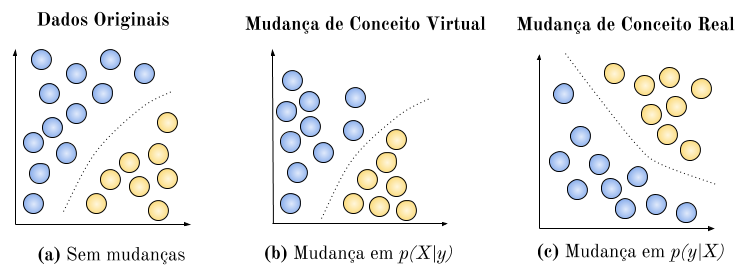
\includegraphics[scale=0.8]{imagens/concept_drift.png}
    \caption{Mudança de Conceito Virtual vs. Mudança de Conceito Real}
    \label{fig:real_and_virtual_concept_drift}
\end{center}
\end{figure}

Conforme \citeonline{Zliobaite:2010}, as mudanças de conceito podem ocorrer de forma abrupta, gradual, incremental ou recorrente.
A Figura \ref{fig:concept_drift_patterns} ilustra estes padrões, 
utilizando círculos na cor azul para representar o conceito \textit{A} e círculos na cor bege para o conceito \textit{B}:

\begin{figure}[H]
\begin{center}
    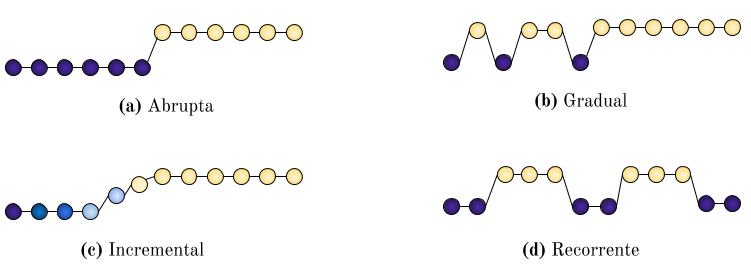
\includegraphics[scale=0.8]{imagens/concept_drift_patterns.png}
    \caption{Padrões de ocorrência de Mudanças de Conceito}
    \label{fig:concept_drift_patterns}
\end{center}
\end{figure}

Na mudança abrupta, o conceito \textit{A} é repentinamente substituído pelo conceito \textit{B} (Figura \ref{fig:concept_drift_patterns} (a)).

Na mudança gradual, ocorre uma transição mais suave entre os conceitos \textit{A} e \textit{B}.
Inicialmente, eventos pertencentes a ambos os conceitos coexistem.
Com o passar do tempo, os eventos pertencentes ao conceito \textit{A} diminuem de frequência, até pararem de ocorrer.
Por fim, os eventos pertencentes a \textit{B} se tornam predominantes (Figura \ref{fig:concept_drift_patterns} (b)).

A mudança incremental descreve a evolução de um único conceito ao longo do tempo.
Essa evolução pode ser discretizada como uma sequência de conceitos consecutivos.
Nesta sequência, cada conceito intermediário difere pouco dos seus conceitos antecessor e sucessor.
Portanto, as mudanças são notáveis apenas à longo prazo (Figura \ref{fig:concept_drift_patterns} (c)).

A mudança recorrente acontece quando um conceito anteriormente ativo reaparece após um determinado período de tempo. 
Contudo, não se trata de uma sazonalidade periódica, pois não é evidente o momento no qual o conceito voltará a ser ativo (Figura \ref{fig:concept_drift_patterns} (d)).

Este trabalho de mestrado propõe um método baseado em redes de função de base radial para detecção de mudanças de conceito em fluxos contínuos de dados, independente do padrão de ocorrência.
Na próxima subseção, será apresentada a terminologia do fenômeno mudança de conceito.

\subsection{Terminologia}

O fenômeno mudança de conceito tem sido estudado em diferentes comunidades de pesquisa, incluindo mineração de dados, 
aprendizado de máquina, estatística e recuperação de informação \cite{Zliobaite:2010}.
Contudo, o tema apresenta diferentes nomeclaturas em cada comunidade.
Na Tabela \ref{tbl:taxonomy} são listados os termos correspondentes a mudança de conceito em cada área de pesquisa.

\begin{table*}[!ht]
    \caption{Terminologia - Mudança de Conceito \cite{Zliobaite:2010}}
    \label{tbl:taxonomy}
    \centering
    \resizebox{\textwidth}{!}{%
    \begin{tabular}[t]{ll}
    \toprule
    Área & Termos \\
    \midrule
    Mineração de Dados                  & Mudança de Conceito                        \\
    Aprendizado de Máquina              & Mudança de Conceito, Mudança de Covariável \\
    Computação Evolucionária            & Ambiente Evolutivo, Ambiente em Mudança    \\
    IA e Robótica                       & Ambiente Dinâmico                          \\
    Estatística, Séries Temporais      & Não Estacionário                           \\
    Recuperação de Informação           & Evolução Temporal                          \\
    \bottomrule
    \end{tabular}%
    }
\end{table*}

Outra fonte comum de equívocos são os termos detecção de \textit{outliers}, detecção de novidade, detecção de \textit{change points} e detecção de mudança de conceito.
Estes termos são muitas vezes utilizados de forma indistinta, mas, para o contexto deste trabalho, é importante distingui-los.

As técnicas para detecção de \textit{outliers} têm como objetivo identificar padrões de dados em desacordo com o comportamento esperado. Estes padrões são geralmente classificados como anomalias ou ruídos \cite{Chandola:2009:ADS:1541880.1541882}.

Os métodos para detecção de novidade identificam padrões ainda não observados, mas que se enquadram no comportamento esperado.
Estes métodos se diferenciam das técnicas para detecção de \textit{outliers} pois os novos padrões são incorporados ao modelo \cite{Chandola:2009:ADS:1541880.1541882}.

As estratégias para detecção de \textit{change points} identificam variações abruptas de valor, que podem representar transições entre estados, em séries temporais unidimensionais estacionárias \cite{Aminikhanghahi:2017:SMT:3086013.3086037}.

Por fim,  cabe definir o que é detecção de mudança de conceito.
Este termo abrange técnicas que monitoram a distribuição dos dados ou indicadores produzidos pelas técnicas de aprendizado aplicadas, com o objetivo de identificar variações que possam impactar a acurácia do modelo em uso \cite{Gama:2014:SCD:2597757.2523813}.

Na próxima subseção, os principais algoritmos para detecção de mudança de conceito serão discutidos.

\subsection{Algoritmos para Detecção de Mudança de Conceito}

Os algoritmos para detecção de mudança de conceito caracterizam e quantificam as mudanças de conceito através da delimitação dos instantes ou intervalos de tempo em que as mudanças ocorrem \cite{Basseville:1993:DAC:151741}.

Esses algoritmos se dividem em duas categorias, conforme a necessidade de rotulação dos dados \cite{Zliobaite:2010}:

\begin{description}
    \item[Algoritmos Explícitos/Supervisionados] Dependem da rotulação dos dados por um especialista.
    Estes rótulos são utilizados no cálculo de medidas de performance como taxa de erro e acurácia, que são monitoradas ao longo do tempo.
    Mudanças de conceito são sinalizadas quando essas medidas atingem um limite previamente definido.

    \item[Algoritmos Implícitos/Não Supervisionados] Independem da rotulação por especialistas.
    As mudanças de conceito são detectadas a partir do monitoramento de características dos próprios dados ou de indicadores produzidos pelas técnicas de aprendizado aplicadas.
    Apesar de serem mais propensos a alarmes falsos, são uma alternativa para cenários onde a obtenção de rótulos é dispendiosa, demorada ou inviável.
\end{description}

Segundo \citeonline{Gama:2014:SCD:2597757.2523813}, os algoritmos \textit{explícitos / supervisionados} podem ser segmentados em três subcategorias:

\begin{description}
    \item[Métodos Baseados em Análise Sequencial] Avaliam continuamente os indicadores de performance (por exemplo: taxa de erro) do algoritmo de aprendizado aplicado.
    A mudança de conceito é detectada quando esses indicadores atingem um limite pré-definido.
    Os algoritmos \textit{Cumulative Sum (CUSUM)}, \textit{PageHinkley (PH)} \cite{Page:CUSUM:PageHinkley:1954} e \textit{Geometric Moving Average (GMA)} \cite{Roberts:2000:CCT:338441.338464}
    são representantes desta subcategoria.

    \item[Abordagens baseadas em Estatística] Identificam mudanças de conceito através da análise de parâmetros estatísticos como média e desvio padrão associados aos resultados das predições.
    Os métodos \textit{Drift Detection Method (DDM)} \cite{GamaMCR04}, 
    \textit{Early Drift Detection Method (EDDM)} \cite{EDDM}, 
    \textit{Exponentially Weighted Moving Average (EWMA)} \cite{Ross:2012:EWM:2076039.2076307} e 
    \textit{Reactive Drift Detection Method (RDDM)} \cite{Barros:RDDM:2017} são exemplos desta subcategoria.

    \item[Métodos baseados em Janelas] Utilizam uma janela de tamanho fixo para sumarizar informações passadas e uma janela deslizante para sumarizar os dados recentes.
    Uma diferença significativa entre as distribuições dessas janelas implica na ocorrência de mudança de conceito.
    Esta diferença é verificada a partir de testes estatísticos ou desigualdades matemáticas, considerando como hipótese nula a igualdade das distribuições.
    Os algoritmos 
    \textit{Adaptive Windowing (ADWIN)} \cite{BifetG07}, 
    \textit{SeqDrift} \cite{PearsSK14:SeqDrift:2014}, 
    \textit{HDDMA} e \textit{HDDMW} \cite{BlancoCRBDM15:HDDMA:HDDMW:2015}
    pertencem a esta subcategoria.
\end{description}

De forma similar, os algoritmos \textit{implícitos / não supervisionados} também foram divididos em três subcategorias \cite{GONCALVES20148144}:

\begin{description}
    \item[Detecção de Novidade / Métodos de Agrupamento] 
    Utilizam técnicas derivadas dos métodos de agrupamento e de detecção de \textit{outliers} para identificar padrões ainda não observados.
    A partir dessa identificação, são realizados cálculos de distância e/ou densidade para confirmar a ocorrência de mudança de conceito \cite{Ryu:Kantardzic:2012}.
    Os métodos 
    \textit{OLINDDA} \cite{Spinosa:2007:OCA:1244002.1244107},
    \textit{MINAS} \cite{Faria:2013:NDA:2480362.2480515},
    \textit{Woo} \cite{Ryu:Kantardzic:2012},
    \textit{DETECTNOD} \cite{Hashemi:Hayat:DETECTNOD:2010},
    \textit{ECSMiner} \cite{Masud:2011:CNC:1978259.1978529} e
    \textit{GC3} \cite{Sethi2016b:GC3} fazem parte desta subcategoria.
    
    \item[Monitoramento de distribuição multivariada]
    Monitoram diretamente a distribuição dos dados para cada atributo.
    A distribuição de um conjunto de treinamento é sumarizada e utilizada como referência.
    Esta referência é, então, comparada à distribuição dos dados do conjunto atual.
    Diferenças significativas entre esses conjuntos indicam a ocorrência de mudança de conceito.
    Os algoritmos
    \textit{CoC} \cite{Lee:Magoules:CoC:2012},
    \textit{HDDDM} \cite{Ditzler:Polikar:HDDDM:2011},
    \textit{PCA-detect} \cite{Kuncheva:PCADetect:20085}
    são representantes desta subcategoria.

    \item[Monitoramento dependente de modelo]
    Requerem a aplicação de um algoritmo de classificação probabilístico, 
    pois as mudanças de conceito são detectadas a partir do monitoramento da probabilidade a posteriori calculada \cite{Zliobaite:2010}.
    Esta restrição permite reduzir a ocorrência de falsos positivos e torna o processo computacionalmente eficiente, pois apenas um único fluxo univariado de valores é observado. 
    Os métodos 
    \textit{A-distance} \cite{Dredze:ADistance:2010585},
    \textit{CDBD} \cite{Lindstrom:CDBD:2013} e
    \textit{Margin} \cite{Dries:Margin:2009} integram esta subcategoria.
\end{description}

Por fim, a Tabela \ref{tbl:abordagens} resume as categorias, as subcategorias e as técnicas apresentadas.
O método de detecção proposto neste trabalho se enquadra na categoria de algoritmos \textit{implícitos / não supervisionados}, mais especificamente na subcategoria \textit{detecção de novidades / métodos de agrupamento}.
Na próxima seção, as ferramentas utilizadas para implementação e validação deste método serão apresentadas.

\begin{table}[ht]
    \caption{Resumo - Algoritmos de detecção \cite{Sethi:2017:RDC:3096751.3096864}}
    \label{tbl:abordagens}
    \centering
    \resizebox{\textwidth}{!}{%
    \begin{tabular}[t]{@{}lllll@{}}
    \toprule
    Categoria & Subcategoria & Algoritmos \\
    \midrule 
    Algoritmos Explícitos/Supervisionados     & Métodos Baseados em Análise Sequencial        & \begin{tabular}[t]{@{}l@{}} Cumulative Sum (CUSUM) \\ PageHinkley (PH) \cite{Page:CUSUM:PageHinkley:1954} \\ Geometric Moving Average (GMA) \cite{Roberts:2000:CCT:338441.338464}\end{tabular}                                                                                                                        &  &  \\
    \addlinespace[2mm]
                                              & Abordagens baseadas em Estatística            & \begin{tabular}[t]{@{}l@{}} Drift Detection Method (DDM) \cite{GamaMCR04} \\  Early Drift Detection Method (EDDM) \cite{EDDM} \\  Exponentially Weighted Moving Average (EWMA) \cite{Ross:2012:EWM:2076039.2076307} \\ Reactive Drift Detection Method (RDDM) \cite{Barros:RDDM:2017} \end{tabular}                   &  &  \\
    \addlinespace[2mm]
                                              & Métodos baseados em Janelas                   & \begin{tabular}[t]{@{}l@{}} Adaptive Windowing (ADWIN) \cite{BifetG07} \\   SeqDrift \cite{PearsSK14:SeqDrift:2014} \\   HDDMA/HDDMW \cite{BlancoCRBDM15:HDDMA:HDDMW:2015} \end{tabular}                                                                                                                              &  &  \\
    \addlinespace[2mm]

    Algoritmos Implícitos/Não Supervisionados & Detecção de Novidade / Métodos de Agrupamento & \begin{tabular}[t]{@{}l@{}} OLINDDA \cite{Spinosa:2007:OCA:1244002.1244107} \\   MINAS \cite{Faria:2013:NDA:2480362.2480515} \\   Woo \cite{Ryu:Kantardzic:2012} \\   DETECTNOD \cite{Hashemi:Hayat:DETECTNOD:2010} \\   ECSMiner \cite{Masud:2011:CNC:1978259.1978529} \\   GC3 \cite{Sethi2016b:GC3} \end{tabular}  &  &  \\
    \addlinespace[2mm]
                                              & Monitoramento de distribuição multivariada    & \begin{tabular}[t]{@{}l@{}} CoC \cite{Lee:Magoules:CoC:2012} \\ HDDDM \cite{Ditzler:Polikar:HDDDM:2011} \\ PCA-detect \cite{Kuncheva:PCADetect:20085} \end{tabular}                                                                                                                                                   &  &  \\
    \addlinespace[2mm]
                                              & Monitoramento dependente de modelo            & \begin{tabular}[t]{@{}l@{}} A-distance \cite{Dredze:ADistance:2010585} \\ CDBD \cite{Lindstrom:CDBD:2013} \\ Margin \cite{Dries:Margin:2009} \end{tabular}                                                                                                                                                            &  &  \\
    \bottomrule
    \end{tabular}%
    }
\end{table}

\subsection{Ferramentas}

Nesta seção, os frameworks \textit{Massive Online Analysis} (MOA) e \textit{Tornado} serão apresentados.
Estes frameworks foram utilizados neste projeto de mestrado para a implementação e validação da técnica proposta.
Além disso, essas ferramentas também foram utilizadas para comparar o algoritmo desenvolvido com o estado da arte, 
pois possuem implementações para os principais métodos existentes na literatura.

\subsection{MOA} 

Atualmente, o \textit{MOA – Massive Online Analysis}\footnote{https://moa.cms.waikato.ac.nz/} é o principal framework para mineração de dados em fluxos contínuos \cite{Bifet:2010:MMO:1756006.1859903}.
O projeto é de código-aberto\footnote{https://github.com/Waikato/moa} e apresenta uma comunidade bastante ativa e crescente.
A aplicação é composta por uma ampla coleção de algoritmos da área de aprendizado de máquina, contemplando técnicas de classificação, regressão, agrupamento, busca por padrões, detecção de \textit{outliers}, detecção de mudanças de conceito e sistemas de recomendação.
Além das implementações, também estão disponíveis rotinas para avaliação dessas técnicas.
A aplicação é desenvolvida em Java, o que permite a sua execução nos principais sistemas operacionais e a integração com o projeto WEKA \cite{Hall:2009:WDM:1656274.1656278}.

O MOA divide as suas funcionalidades em tarefas (\textit{tasks}).
Estas tarefas podem ser executadas a partir da interface gráfica (GUI) ou por linha de comando.
A interface gráfica permite executar múltiplas tarefas de forma concorrente, 
controlar suas execuções e visualizar os resultados parciais.
A tela principal da aplicação é demonstrada na Figura \ref{fig:moa}.

\begin{figure}[H]
\begin{center}
    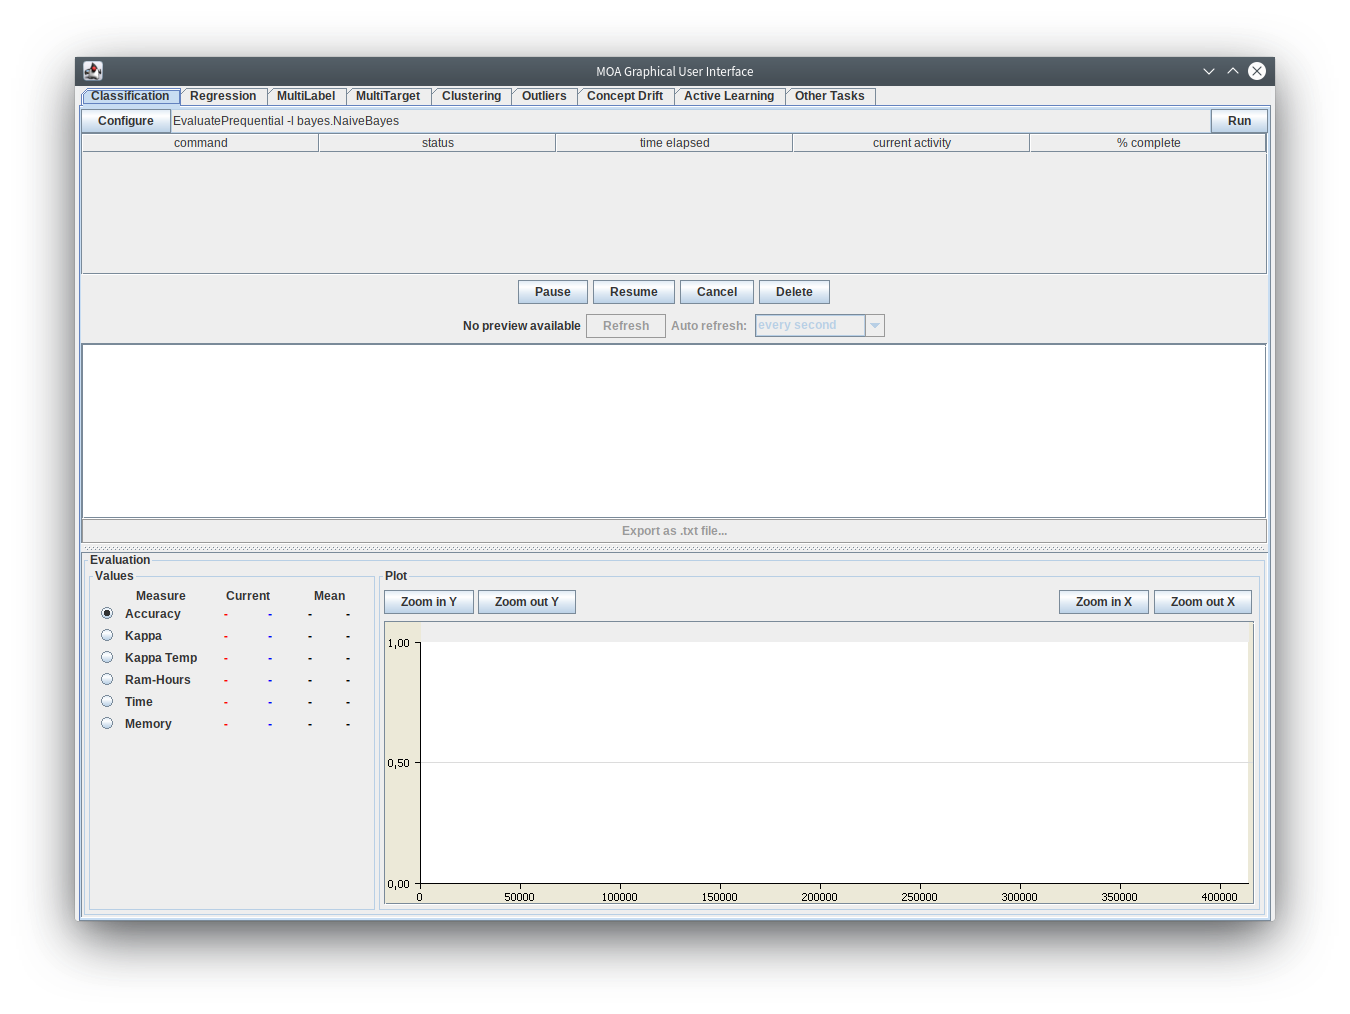
\includegraphics[scale=0.4]{imagens/moa.png}
    \caption{MOA - Tela Inicial}
    \label{fig:moa}
\end{center}
\end{figure}

A aplicação é capaz de ler arquivos em formato \textit{ARFF}, além de permitir a produção de fluxos de dados dinamicamente, através de geradores.
Alguns dos geradores de fluxo disponíveis no MOA são:
\textit{Random Trees} \cite{Domingos:2000:MHD:347090.347107}
\textit{SEA} \cite{Street:2001:SEA:502512.502568}, 
\textit{STAGGER} \cite{Schlimmer1986}, 
\textit{Rotating Hyperplane} \cite{Wang:2003:MCD:956750.956778},
\textit{Random RBF}, 
\textit{LED} \cite{Gama:2003:ADT:956750.956813}, 
\textit{Waveform} \cite{Gama:2003:ADT:956750.956813}, 
 e \textit{Function} \cite{Jin:2003:EDT:956750.956821}.

Outra funcionalidade importante do framework é a possibilidade de adicionar mudanças de conceito a fluxos estacionários existentes.
Esse processo é realizado através de uma função sigmóide, que modela o evento de mudança de conceito como uma combinação balanceada de duas distribuições homogêneas, 
que caracterizam os conceitos-alvo antes e depois da mudança.
Além destes conceitos, o usuário também pode definir o momento da mudança e a sua duração \cite{Bifet:2010:MMO:1756006.1859903}.

Os principais métodos para detecção de mudança de conceito propostos na literatura estão disponíveis no MOA.
Além disso, a arquitetura do framework é modular, permitindo a implementação de novos detectores de forma trivial.
Por exemplo, para criar um novo detector, basta estender a classe abstrata \textit{AbstractChangeDetector} e implementar o algoritmo desejado.
A janela de configuração deste detector, similar a Figura \ref{fig:moa_detector}, será criada dinamicamente, a partir dos atributos definidos na classe.

\begin{figure}[H]
\begin{center}
    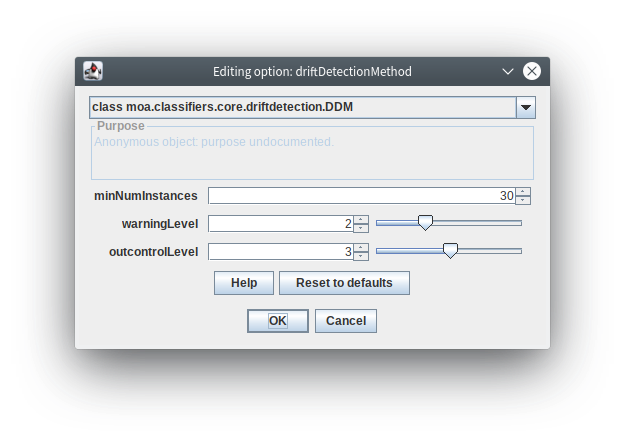
\includegraphics[scale=1]{imagens/detector.png}
    \caption{MOA - Configuração detector}
    \label{fig:moa_detector}
\end{center}
\end{figure}
    
Além de possuir implementações para diversos algoritmos da área de aprendizado de máquina e de áreas correlatas, o framework também dispõe de classes para avaliar a acurácia e a performance dessas técnicas.
Neste trabalho de mestrado, a classe \textit{BasicConceptDriftPerformanceEvaluator} será utilizada para avaliar a acurácia e a performance do método proposto.
Na próxima subseção, o framework \textit{Tornado} será apresentado.

\subsection{Tornado}

O \textit{Tornado} é um framework desenvolvido especificamente para analisar algoritmos de detecção de mudanças de conceito \cite{Pesaranghader:Tornado}.
O projeto é construído na linguagem Python e o seu código está disponível\footnote{https://github.com/alipsgh/tornado}.
O framework se diferencia do \textit{MOA}, pois apresenta um cenário de avaliação próprio:
analisar a execução, em paralelo, de pares formados por um classificador e um detector de mudanças, 
para identificar o par ótimo ao longo do tempo, em relação ao fluxo de dados.

\begin{figure}[ht]
\begin{center}
    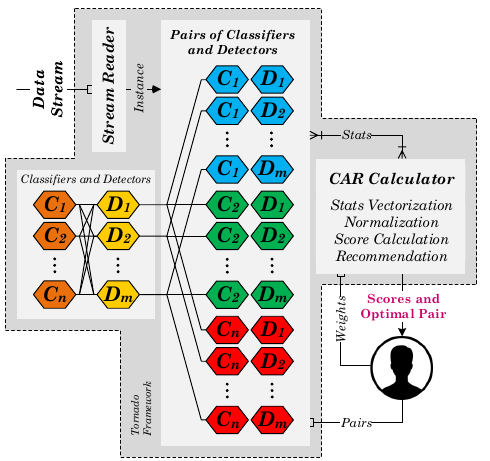
\includegraphics[scale=0.75]{imagens/tornado.png}
    \caption{Framework Tornado \cite{Pesaranghader:Tornado}.}
    \label{fig:tornado}
\end{center}
\end{figure}

Conforme apresentado na Figura \ref{fig:tornado}, os principais componentes do framework são: 
\textit{Stream Reader}, \textit{Classifiers}, \textit{Detectors}, \textit{Classifier-Detector Pairs} e \textit{CAR Calculator}.
A entrada de dados é composta por um fluxo (\textit{Stream}), uma lista de pares (classificador, detector) e um vetor com pesos.
O componente \textit{Stream Reader} recepciona as instâncias e as encaminha para construção do modelo de forma incremental. 
Por seguir a abordagem \textit{prequential}, cada instância é primeiramente utilizada para testes e depois como treinamento.
Simultaneamente, os classificadores enviam suas estatísticas aos detectores, para que a mudança de conceito possa ser sinalizada.
Por fim, o componente \textit{CAR Calculator} calcula uma pontuação para cada par, baseada na taxa de erro, atraso para detecção (\textit{delay}), falsos positivos, falsos negativos, quantidade de memória utilizada e tempo de execução \cite{Pesaranghader:Tornado}.

O resultado produzido identifica o par ótimo para cada instante da execução. 
Esta abordagem de avaliação se mostra relevante, pois o par ideal pode mudar ao longo do tempo, devido ao aprendizado incremental ou às mudanças de conceito.
A Figura \ref{fig:tornado_out2} apresenta um exemplo de resultado da ferramenta.

\begin{figure}[ht]
\begin{center}
    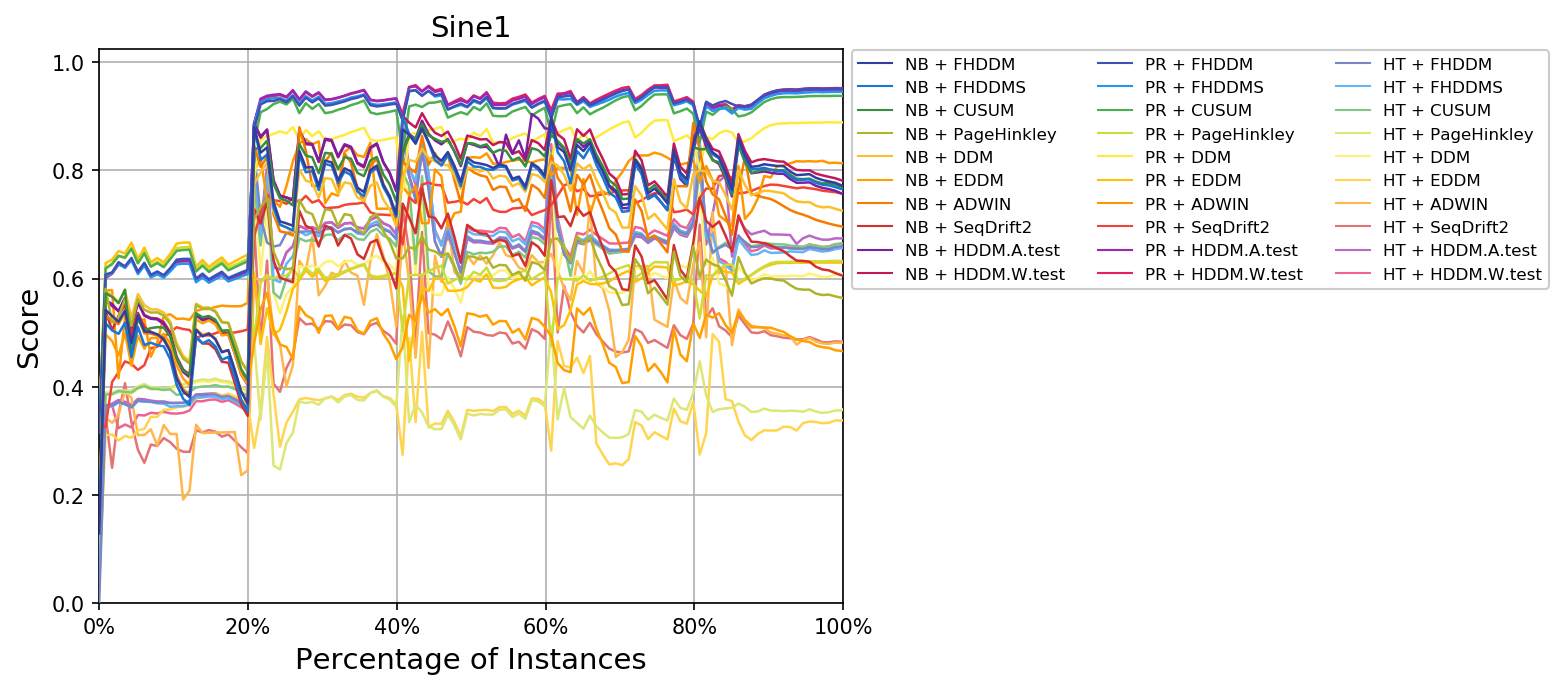
\includegraphics[scale=0.6]{imagens/tornado_out2.png}
    \caption{Tornado - Exemplo de resultado \cite{Pesaranghader:Tornado}}
    \label{fig:tornado_out2}
\end{center}
\end{figure}

Neste trabalho, o algoritmo proposto será implementado e testado nas duas ferramentas apresentadas.
Os detalhes de implementação e os resultados desses testes serão discutidos no Capítulo \ref{experimentos_iniciais}.
A seguir, as redes de função de base radial são detalhadas.

\section{Redes de Função de Base Radial}

Uma Rede de Função de Base Radial (\textit{radial basis function, RBF,} em inglês) pode ser definida como um modelo de múltiplas camadas alimentadas adiante (\textit{feedforward}), 
capaz de analisar padrões complexos e resolver problemas não-linearmente separáveis, utilizando uma abordagem de aproximação de funções.
Estas redes têm como principal diferencial a sua forma de ativação, realizada através do cálculo da distância entre o dado e um centro definido \cite{Braga:RedesNeuraisTeoriaAplicacoes}.

A arquitetura de uma rede de função de base radial, em sua forma mais básica, envolve três camadas.
A camada de entrada conecta a rede ao seu ambiente, recepcionando novos dados.
A camada intermediária, única camada oculta da rede, 
utiliza funções de base radial para realizar uma transformação não-linear dos dados de entrada para um espaço de alta dimensionalidade.
Por fim, a camada de saída, através de uma combinação linear, fornece a resposta final da rede \cite{Rojas:1996:NNS:235222}. 
A Figura \ref{fig:rbg_arq} demonstra essa arquitetura.

\begin{figure}[ht]
\begin{center}
    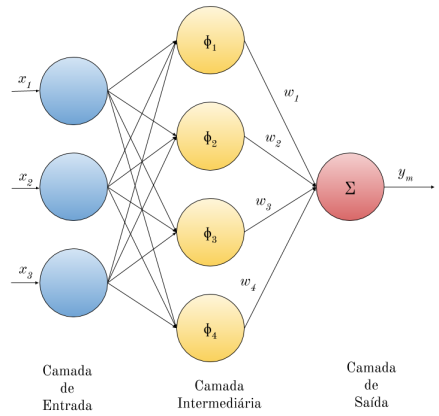
\includegraphics[scale=1]{imagens/rbf_arq.png}
    \caption{Arquitetura RBF}
    \label{fig:rbg_arq}
\end{center}
\end{figure}

A transformação não-linear dos dados de entrada para um espaço de alta dimensionalidade é justificada matematicamente pelo teorema de \citeonline{cover1965browse}, 
segundo o qual, ``um problema complexo de classificação de padrões disposto não linearmente em um espaço de alta dimensionalidade tem maior probabilidade de ser linearmente separável do que em um espaço de baixa dimensionalidade''.

Essa transformação é realizada por funções de base radial presentes na camada intermediária. 
Na literatura, uma das funções mais utilizadas para esta tarefa é a função Gaussiana, representada na Equação \ref{eq:gaussiana}:

\begin{equation}
    \label{eq:gaussiana}
    \varphi (v_{i})=e^{-(\sigma r)^{2}}
\end{equation}

% r=
onde, $r$ é a distância euclidiana ($\|\mathbf {v_{i}} - \mathbf {c_{i}}\|$), $v$ é o valor de entrada, $c_i$ representa o centro e $\sigma$ é o parâmetro limitador do raio.
Assim, a classificação realizada por uma rede de função de base radial consiste na resolução das funções \ref{eq:rbf1} e \ref{eq:rbf2}:

\begin{equation} \label{eq:rbf1}
    f(x)=\sum _{{i=1}}^{N}w_{ij}\varphi (||{\mathbf  {x}}-{\mathbf  {t}}_{i}||)
\end{equation}

\begin{equation} \label{eq:rbf2}
    y_i=\sum _{{i=1}}^{N}w_{ij}\phi (||{\mathbf  {x}}-{\mathbf  {t}}_{i}||) + w_{j_0}
\end{equation}

A resolução dessas equações dá origem ao sistema responsável por produzir o resultado final da rede (Equação \ref{eq:rbf3}):

\begin{equation} \label{eq:rbf3}
\begin{bmatrix}
    \varphi (||{{x_1}}-{{t}}_{1}||) & \varphi (||{{x_1}}-{{t}}_{2}||) & \dots & \varphi (||{{x_1}}-{{t}}_{N}||) \\
    \varphi (||{{x_2}}-{{t}}_{1}||) & \varphi (||{{x_2}}-{{t}}_{2}||) & \dots & \varphi (||{{x_2}}-{{t}}_{N}||) \\
    \hdotsfor{5} \\
    \varphi (||{{x_N}}-{{t}}_{1}||) & \varphi (||{{x_N}}-{{t}}_{2}||) & \dots & \varphi (||{{x_N}}-{{t}}_{N}||)
\end{bmatrix}
\begin{bmatrix}
    w_1 \\
    w_2 \\
    \vdots \\
    w_N \\
\end{bmatrix}
=
\begin{bmatrix}
    y_1 \\
    y_2 \\
    \vdots \\
    y_N \\
\end{bmatrix}
\end{equation}

onde $w_{ij}$ são os pesos de cada conexão, $\phi$ é a matriz de interpolação originada do conjunto de $N$ funções
de base radial aplicadas nas entradas $x$ e dos seus respectivos centros $t_i$,
$w_{j_0}$ representa o bias, $\varphi (||{{x}}-{{t}}_{i}||)$ é o conjunto de $N$ funções de base radial,
$||\ldots||$ é a norma euclidiana e $y$ são as saídas geradas pela rede.

O algoritmo proposto neste trabalho utiliza as camadas inicial e intermediária das redes de função de base radial para compôr um novo método de detecção de mudanças de conceito.
Isto é possível, pois a camada intermediária cria, de forma implícita, agrupamentos no espaço oculto de alta dimensionalidade.
Dessa forma, a criação de novos centros e a mudança do centro ativo podem sinalizar a ocorrência de mudanças de conceito.
A técnica desenvolvida será discutida em detalhes no Capítulo \ref{plano_pesquisa}.
Na próxima seção, os trabalhos relacionados encontrados na literatura são apresentados.

\section{Trabalhos Relacionados}

Além das referências básicas apresentadas neste capítulo, foi realizada uma pesquisa na literatura visando identificar trabalhos 
que utilizam redes de função de base radial para identificação de mudanças de conceito ou para outras tarefas correlatas.

\citeonline{Roberts:Penny:Novelty:Confidence} propuseram um método para detecção de novidades baseado em um comitê de redes de função de base radial.
Neste método, novos padrões são detectados a partir do monitoramento das taxas de erro e confiança do comitê.
A técnica foi utilizada para classificação de pacientes com problemas de tremor muscular.

\citeonline{Jianping:Venkateswarlu:RBF:SpeakerIdentification} também utilizaram as redes de função de base radial em tarefas de detecção de novidades.
A técnica proposta atua sobre cenários estacionários e foi aplicada ao problema de identificação da fala.
Seu principal diferencial é a utilização do algoritmo \textit{k-means} para definir os centros e as matrizes de covariância da rede.

Por fim, \citeonline{Bazargani2018RadialBF} utilizaram redes RBF para detecção de anomalias em fluxos de dados.
O método proposto modifica as funções de perda, transformando as redes de função de base radial em classificadores de classe única, 
permitindo a identificação de exemplos divergentes dos padrões conhecidos.

\section{Considerações Finais}

Neste capítulo foram apresentados os principais conceitos utilizados neste projeto de trabalho de mestrado.
Foram discutidos conceitos de fluxos contínuos de dados, 
técnicas de aprendizado de máquina, 
mudança de conceito,
técnicas de detecção e redes de função de base radial.
Por fim, foram apresentados os trabalhos relacionados encontrados na literatura.
No próximo capítulo, o plano de pesquisa será detalhado.

\xchapter{Plano de Pesquisa}{} \label{plano_pesquisa}
\section{Considerações Iniciais}

Este capítulo descreve como a pesquisa proposta neste mestrado será desenvolvida para permitir que redes de função de base radial sejam aplicadas para detectar mudanças de conceito em fluxos contínuos de dados.
Espera-se que com a utilização de redes RBF, seja possível detectar mudanças de conceito em fluxos contínuos em tempo de execução, de forma computacionalmente eficiente e independente de rótulos.
A seguir, são apresentados detalhes sobre cada etapa do desenvolvimento do projeto.

\section{Descrição do Problema}

Nos últimos anos, a quantidade de dados produzidos por sistemas computacionais tem crescido de forma exponencial \cite{idc_report}.
Parte significativa dessas informações é produzida na forma de fluxos contínuos de dados, que são sequências potencialmente infinitas e de alta frequência \cite{Aggarwal:2006:DSM:1196418}.

Devido a esse crescimento, pesquisadores passaram a utilizar técnicas de aprendizado de máquina para extrair informações úteis de grandes volumes de dados.
Essas técnicas precisaram ser adaptadas para contextos com fluxos contínuos, pois estes cenários apresentam severas restrições de tempo de execução e de uso dos recursos computacionais.

Contudo, as adaptações propostas não tratam variações na distribuição dos dados ou no contexto do processo gerador do fluxo.
Estas alterações são denominadas mudanças de conceito e podem afetar negativamente a acurácia do algoritmo \cite{Gama:2014:SCD:2597757.2523813}.

Para mitigar este problema, técnicas de detecção de mudanças de conceito foram desenvolvidas. 
Estes métodos identificam com precisão o momento da mudança, permitindo que o modelo de decisão seja atualizado de forma eficiente e tempestiva.

Entretanto, as técnicas de detecção encontradas na literatura apresentam limitações ao serem aplicadas em cenários com fluxos contínuos de dados.
Os métodos de detecção supervisionados/explícitos necessitam que o rótulo correto de cada exemplo processado seja informado, o que os torna inviáveis, por causa do custo e do tempo de rotulação.
Enquanto as técnicas não supervisionadas/implícitas têm dificuldade para antender às restrições de tempo de execução e de uso dos recursos computacionais desses cenários.

Redes de função de base radial são modelos de redes neurais multicamadas, alimentadas adiante, capazes de analisar padrões complexos e resolver problemas não-linearmente separáveis \cite{Braga:RedesNeuraisTeoriaAplicacoes}.
A arquitetura básica dessas redes é composta por três camadas.
A camada de entrada recepciona os dados.
A camada intermediária, através de funções de base radial, realiza uma transformação não-linear dos dados para um espaço com alta dimensionalidade, buscando tornar o problema linearmente separável \cite{cover1965browse}.
Por fim, a camada de saída produz o resultado final da rede através de uma combinação linear dos resultados da camada intermediária \cite{Rojas:1996:NNS:235222}.

A camada intermediária das redes de função de base radial forma, implicitamente, grupos (\textit{clusters}) no espaço de alta dimensionalidade criado.
O centro ativo deste agrupamento pode se alterar, conforme o valor processado.
Assim, este trabalho de mestrado implementa as camadas inicial e intermediária, 
e utiliza as alterações de centro no espaço de alta dimensionalidade como indicadores da ocorrência de mudanças de conceito.

O método proposto, denominado \textit{RBFDriftDetector}, utiliza a Gaussiana (Equação \ref{eq:gaussiana}) como função de base radial e requer a definição de dois parâmetros: 
\textit{$\sigma$}, responsável por limitar o raio da função gaussiana, e \textit{$\lambda$}, que define o valor mínimo para ativação de um centro.
A técnica é descrita na forma de pseudocódigo em Algoritmo \ref{alg:algoritmo}, 
tendo sido também implementada na linguagem Java\footnote{\url{https://git.io/fjGuv}}, para realização dos experimentos na plataforma MOA.

\vspace{7pt}
\begin{algorithm}[H]
    \SetAlgoLined
    \Entrada{$valor, \sigma, \lambda$} 
    \Saida{booleano indicando a ocorrência ou não de mudança de conceito}
    \Inicio{
     $centros \longleftarrow ()$; $centroAtual \longleftarrow null$; $centroAtivo \longleftarrow null$\\
     $mudanca \longleftarrow falso$

     \ParaTodo{centro}{
         $ativacao \longleftarrow gaussiana(valor, centro, \sigma)$\\
         \Se{$ativacao >= \lambda$}{
            $centroAtivo \longleftarrow centro$ \\
            $\lambda \longleftarrow ativacao$ \\ 
         }
    } 
    \Se{$centroAtivo == null$}{
        $centros \longleftarrow valor$ \\    
        $centroAtivo \longleftarrow valor$ \\
    }   
    \Se{$centroAtual \neq centroAtivo$}{
        $centroAtual \longleftarrow centroAtivo$ \\
        $mudanca \longleftarrow verdadeiro$ \\
    }
    \Retorna{mudanca}\\
    \BlankLine
    \BlankLine
    }

    \caption{\textsc{RBFDriftDetector}}
    \label{alg:algoritmo} 
\end{algorithm}
\vspace{7pt}

Para exemplificar a execução do algoritmo proposto neste projeto, considere o conjunto $S = \{0.11, 0.12, 0.13, 0.34, 0.45, 0.47, 0.33, 0.25, 0.14, 0.10\}$ como fonte de dados.
Para este exemplo, os parâmetros foram definidos de forma empírica. O parâmetro \textit{$\sigma$} foi definido com o valor $0.2$ e o parâmetro \textit{$\lambda$} foi fixado em $0.6$.
A seguir, será descrito o comportamento do algoritmo para cada dado recebido a partir de $S$.

No instante $T1$, o valor $0.11$ é recepcionado. Como não existem centros estabelecidos, o valor é definido como centro e ativado.
Em $T2$ e $T3$ são recebidos, respectivamente, os valores $0.12$ e $0.13$ que são imediatamente vinculados ao centro atualmente ativo ($0.11$), pois seus valores de ativação foram maiores que $0.6$ ($\lambda$).

No instante $T4$, o valor $0.34$ não atinge o valor mínimo de ativação (\textit{$\lambda$}) para ser vinculado ao centro ativo ($0.11$). 
Dessa forma, o valor é definido como um novo centro e ativado.
Devido a alteração do centro ativo, o algoritmo sinaliza a ocorrência de mudança de conceito.

Os valores dos instantes $T5$, $T6$, $T7$ e $T8$ são vinculados ao último centro ativo ($0.34$). 
Contudo, em $T9$, o valor $0.14$ é recebido e apresenta maior valor de ativação para o centro $0.11$, que é reativado. 
Assim, uma nova mudança de conceito é sinalizada.
Finalmente, o valor do instante $T10$, $0.10$, é vinculado ao centro ativo ($0.11$).

A Figura \ref{fig:funcionamento_algoritmo} apresenta esse comportamento graficamente. 
Os círculos na cor amarela representam valores vinculados ao primeiro centro estabelecido ($0.11$ no momento $T1$), 
enquanto os de cor lilás foram ativados pelo segundo centro definido ($0.34$ em $T4$).
As linhas verticais tracejadas, de cor vermelha, indicam a ocorrência de mudança de conceito.

\begin{figure}[H]
\begin{center}
    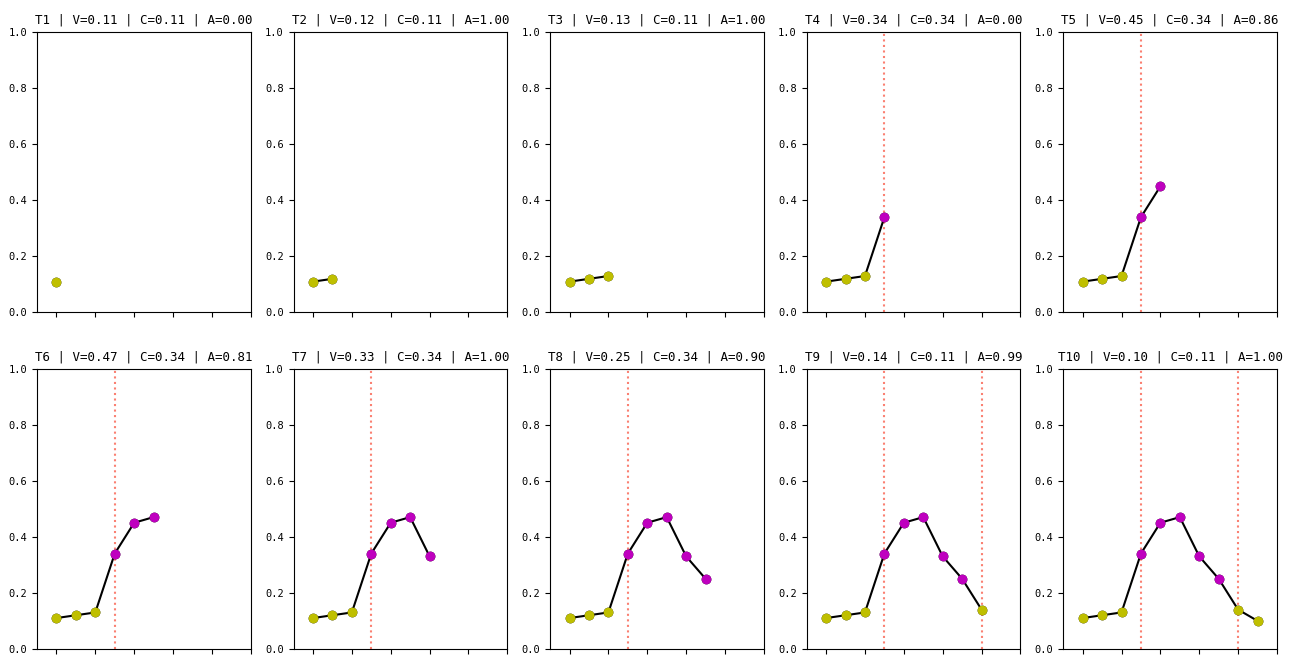
\includegraphics[width=\textwidth]{imagens/funcionamento_algoritmo.png}
    \caption{Exemplo de funcionamento do algoritmo}
    \label{fig:funcionamento_algoritmo}
\end{center}
\end{figure}

\section{Atividades de Pesquisa}

A Tabela \ref{cronograma} apresenta o cronograma das atividades planejadas para a realização da pesquisa. Atividades concluídas são representadas pelo símbolo $X$ e as futuras por $\bullet$. 

\begin{table}[htbp]
\begin{center}
\caption{Cronograma de atividades}     % mude aqui para seu título da tabela
\label{cronograma} % para referencia no texto.
\resizebox{\textwidth}{!}{ % abre resizebox, setar tabela da largura da página.
\begin{tabular}{|c|l|l|l|l|l|l|l|l|l|l|l|l|l|l|l|l|l|l|l|l|l|l|l|l|}
\hline
\multicolumn{1}{|c|}{\multirow{2}{*}{Atividades}} & \multicolumn{24}{c|}{Meses} \\ \cline{2-25}
\multicolumn{1}{|c|}{} & 01 & 02 & 03 & 04 & 05 & 06 & 07 & 08 & 09 & 10 & 11 & 12 & 13 & 14 & 15 & 16 & 17 & 18 & 19 & 20 & 21 & 22 & 23 & 24 \\ \hline
%\rowcolor[HTML]{EFEFEF}

1-Disciplinas & X & X & X & X & X & X & X & X & X & X & ~ & ~ & ~ & ~ & ~ & ~ & ~ & ~ & ~ & ~ & ~ & ~ & ~ & ~ \\ \hline
2-Revisão da Literatura & ~ & ~ & ~ & ~ & ~ & ~ & X & X & X & X & X & X & ~ & ~ & ~ & ~ &  ~ & ~ & ~ & ~ & ~ & ~ & ~ & ~ \\ \hline
3-Experimentos  & ~ & ~ & ~ & ~ & ~ & ~ & ~ & ~ & X & X & X  & X & $\bullet$ & $\bullet$ & $\bullet$ & $\bullet$ & ~ & ~ & ~ & ~ & ~ & ~ & ~ & ~ \\ \hline
4-Análise dos Resultados & ~ & ~ & ~ & ~ & ~ & ~ & ~ & ~ & ~ & ~ & X & X & ~  & ~  & ~ & $\bullet$ & $\bullet$ & $\bullet$ & ~ & ~ & ~ & ~ & ~ & ~ \\ \hline
5-Escrita da qualificação & ~ & ~ & ~ & ~ & ~ & ~ & ~ & ~ & ~ & X & X & X & ~ & ~ & ~ & ~ & ~ & ~ & ~ & ~ & ~ & ~ & ~ & ~ \\ \hline
6-Estágio docente & ~ & ~ & ~ & ~ & ~ & ~ & ~ & ~ & ~ & ~ & ~ & ~ & ~ & ~ & ~ & $\bullet$ & $\bullet$ & $\bullet$ & $\bullet$ & $\bullet$ & $\bullet$ & ~ & ~ & ~ \\ \hline
7-Pesquisa Orientada & ~ & ~ & ~ & ~ & ~ & ~ & X & X & X & X & X & X & $\bullet$ & $\bullet$ & $\bullet$ & $\bullet$ & $\bullet$ & $\bullet$ & $\bullet$ & $\bullet$ & $\bullet$ & $\bullet$ & $\bullet$ & $\bullet$ \\ \hline
8-Apresentação da qualificação & ~ & ~ & ~ & ~ & ~ & ~ & ~ & ~ & ~ & ~ & ~ & ~ & $\bullet$ & ~ & ~ & ~ & ~ & ~ & ~ & ~ & ~ & ~ & ~ & ~ \\ \hline
9-Escrita de artigos& ~ & ~ & ~ & ~ & ~ & ~ & ~ & ~ & ~ & ~ & ~ & ~ & ~  & ~ & ~ & ~ & ~ & $\bullet$ & $\bullet$ & ~ & ~ & ~ & ~ & ~ \\ \hline
10-Escrita da dissertação& ~ & ~ & ~ & ~ & ~ & ~ & ~ & ~ & ~ & X & X & X & ~ & ~ & ~ & ~ & $\bullet$ & $\bullet$ & $\bullet$ & $\bullet$ & $\bullet$ & $\bullet$ & $\bullet$ & $\bullet$ \\ \hline
11- Defesa da dissertação& ~ & ~ & ~ & ~ & ~ & ~ & ~ & ~ & ~ & ~ & ~ & ~ & ~ & ~ & ~ & ~ & ~ & ~ & ~ & ~ & ~ & ~ & ~ & $\bullet$ \\ \hline

\hline
\end{tabular}
} % fecha resizebox
\end{center}
\end{table}

Para a conclusão da atividade 1, 
o Programa de Pós-Graduação em Ciência da Computação (PGCOMP) da Universidade Federal da Bahia (UFBA) exige que um mestrando obtenha um total de 18 créditos em disciplinas. 
Nos semestres 2018.1 e 2018.2, foram obtidos os créditos exigidos ao cursar as disciplinas: 
MATD74 -- Algoritmos e Grafos, MATE32 -- Tópicos em Inteligência Computacional II, MATE64 -- Seminários Científicos, MATE65 -- Fundamentos de Pesquisa em Ciência da Computação I,
MATE10 -- Tópicos em Inteligência Computacional I e MATE84 -- Tópicos em Fundamentos da Computação IV.

A segunda atividade planejada neste cronograma foi realizada a partir da disciplina MATE65 -- Fundamentos de Pesquisa em Ciência da Computação I 
e nos meses subsequentes. Além disso, durante a execução desta tarefa foi realizada a prova de proficiência em inglês.

As atividades 3 e 4 do cronograma consistem na realização dos experimentos e análise dos resultados. 
Essas atividades foram divididas em duas partes. 
A primeira contém apenas experimentos preliminares que foram realizados para validar esta proposta de trabalho. 
Nesta parte, fluxos contínuos de dados sintéticos com mudança de conceito foram analisados conforme apresentado no Capítulo \ref{experimentos_iniciais}. 
A segunda parte dos experimentos e suas análises serão realizadas após a qualificação.

As atividades 5 e 8 estão relacionadas com o componente curricular MATD75 -- Exame de qualificação. A atividade 5 refere-se à escrita deste texto e as atividades 6 e 7 representam os componentes curriculares MATA32 -- Estágio Docente e MATA31 -- Pesquisa Orientada, respectivamente. A atividade 8 está relacionada à apresentação desta qualificação de mestrado.
 
A escrita de artigos, listada no item 9 do cronograma, será realizada com base nos resultados gerados com os experimentos (Atividades $3$ e $4$) e nas contribuições obtidas com a apresentação da qualificação. Por fim, como requisito para a defesa de dissertação, fica pendente a atividade MATE93 -– Defesa de Proposta de Mestrado, a qual se refere aos itens 10 e 11 da Tabela \ref{cronograma}. 

\section{Considerações Finais}

Neste capítulo, apresentou-se de maneira detalhada o projeto de pesquisa, o plano de atividades e o cronograma planejado para a conclusão do mestrado. 
No próximo capítulo, serão discutidos os resultados preliminares realizados com o objetivo de analisar a viabilidade da proposta de mestrado.

\xchapter{Experimentos Iniciais}{} \label{experimentos_iniciais}
\section{Considerações Iniciais}

Este capítulo apresenta um conjunto de experimentos preliminares realizados com dados sintéticos, cujo objetivo foi demonstrar a viabilidade da proposta de mestrado.
%
Os resultados obtidos se mostraram promissores, indicando que o tema de pesquisa deve continuar a ser investigado.
%
A próxima seção apresenta como os dados sintéticos foram produzidos para condução dos experimentos.

\section{Configuração dos Experimentos}
\label{sec:configuracao_experimentos}

Os fluxos de dados sintéticos foram produzidos através de classes geradoras do framework \textit{MOA} e salvos em arquivos no formato \textit{ARFF}, para que pudessem ser reutilizados entre os experimentos.
Cada fluxo produzido representa até dois conceitos e é composto por 2.500 observações, com valores entre 0 e 1.
O restante desta seção apresenta as classes geradoras utilizadas, as modificações realizadas e os parâmetros aplicados.

A classe geradora \textit{AbruptChangeGenerator} produz fluxos de dados sintéticos com mudanças de conceito abruptas.
Os fluxos gerados simulam as mudanças através da intercalação de sequências com o valor $0.2$ e sequências com o valor $0.8$, conforme o tamanho definido para os conceitos.
Com o objetivo de tornar os dados produzidos mais próximos da realidade, a classe foi alterada\footnote{\url{https://git.io/fjGEj}} para permitir a adição de um ruído randômico, com amplitude configurável, para cada exemplo produzido.
A versão com suporte a ruído foi utilizada na produção do fluxo com mudanças abruptas utilizado nos experimentos.
O gerador foi parametrizado para produzir exemplos não binários, com conceitos formados por 400 instâncias e ruído limitado ao intervalo $[-0.1, 0.2]$.

% Esta configuração é apresentada na Figura \ref{fig:abrupt_change_generator}.

% \begin{figure}[H]
%     \begin{center}
%         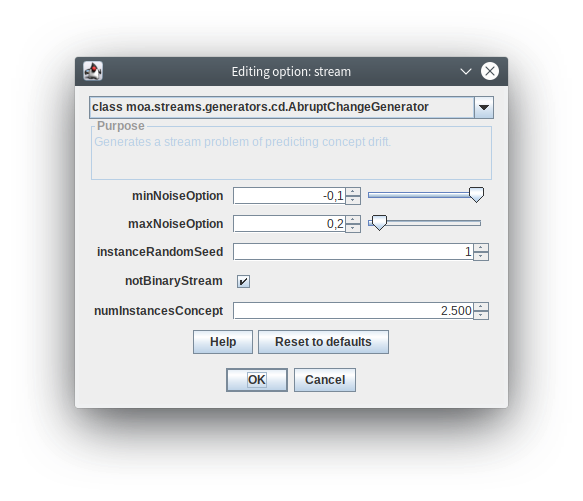
\includegraphics[width=\textwidth]{imagens/abrupt_change_generator.png}
%         \caption{Parametrização da classe \textit{AbruptChangeGenerator}}
%         \label{fig:abrupt_change_generator}
%     \end{center}
% \end{figure}

A classe \textit{GradualChangeGenerator} produz fluxos sintéticos com mudanças de conceito graduais.
Durante sua configuração, percebeu-se uma limitação, pois a classe só gera uma mudança gradual, independente do tamanho dos conceitos.
Para mitigar esta limitação, a classe foi modificada\footnote{\url{https://git.io/fjGue}} para gerar uma quantidade de mudanças coerente com o tamanho definido.
A classe modificada foi utilizada para gerar o fluxo sintético com mudanças graduais utilizado nos experimentos, 
sendo parametrizada para produzir exemplos não binários e conceitos compostos por 400 instâncias.

% A Figura \ref{fig:gradual_change_generator} apresenta a tela de configuração da aplicação.

% \begin{figure}[H]
%     \begin{center}
%         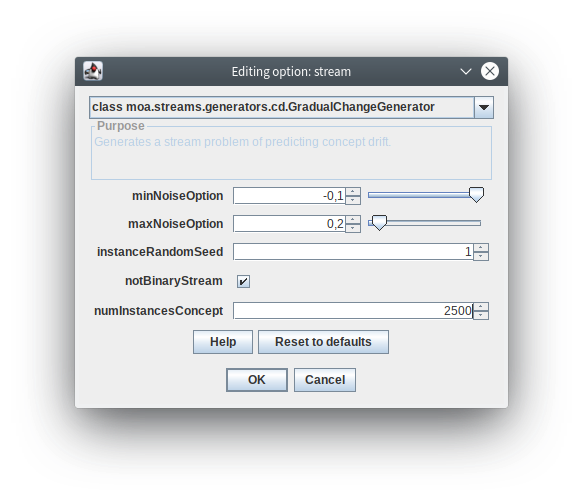
\includegraphics[width=\textwidth]{imagens/gradual_change_generator.png}
%         \caption{Parametrização da classe \textit{GradualChangeGenerator}}
%         \label{fig:gradual_change_generator}
%     \end{center}
% \end{figure}

Por fim, a classe \textit{NoChangeGenerator}, que produz fluxos sem ocorrência de mudanças de conceito, também foi modificada\footnote{\url{https://git.io/fjGu3}} para permitir a incidência de ruído nos resultados gerados.
Esta versão foi utilizada para produzir um fluxo sintético sem mudanças, com ruído entre $[-0.1, 0.1]$, para ser utilizado como \textit{baseline} nos experimentos.

\section{Critérios de avaliação}

A classe de avaliação \textit{BasicConceptDriftPerformanceEvaluator}, pertencente ao framework \textit{MOA}, será utilizada para avaliar o método proposto neste trabalho.
Esta classe permite mensurar a acurácia e o desemprenho de algoritmos para detecção de mudanças de conceito.
Para utilizá-la, é necessário construir uma tarefa do tipo \textit{EvaluateConceptDrift} através da aba \textit{Concept Drift}, presente na tela inicial da aplicação.

Para condução dos experimentos deste trabalho de mestrado, a classe foi configurada conforme descrito na Tabela \ref{tbl:configuracao_tarefa}.

\begin{center} 
    \begin{table}[h]
    \caption{Configuração da classe \textit{BasicConceptDriftPerformanceEvaluator}}
    \label{tbl:configuracao_tarefa}
    \resizebox{\textwidth}{!} {%
    \begin{tabular}{llm{7.5cm}}
    \toprule
    Parâmetro & Valor & Observação \\
    \midrule
    learner          & ChangeDetectorLearner  &  O algoritmo de detecção de mudanças de conceito a ser testado é definido no atributo \textit{driftDetectionMethod} da classe \textit{ChangeDetectorLearner}.                   \\
    stream           & ARFFFileStream         &  Caminho para um dos arquivos \textit{ARFF} descrito na seção anterior. O atributo \textit{classIndex} deve ser definido como $0$, pois não existem rótulos nestes conjuntos de dados.  \\ 
    instanceLimit    & $-1$                            &  Desabilita o limite de instâncias a serem processadas.  \\
    timeLimit        & $-1$                            &  Desabilita o limite de tempo de execução.  \\ 
    sampleFrequency  & \hspace{3mm}$1$                 &  Uma linha de resultado do avaliador deve ser gerada para cada instância processada.  \\
    \bottomrule
    \end{tabular}
    }
    \end{table}
\end{center}

A classe de avaliação utilizada produz diversos indicadores referentes a acurácia e performance do algoritmo executado. 
A Tabela \ref{tbl:indicadores_analisado} apresenta os indicadores analisados neste trabalho.

\begin{center} 
    \begin{table}[h]
    \caption{Indicadores analisados}
    \label{tbl:indicadores_analisado}
    \resizebox{\textwidth}{!} {%
    \begin{tabular}{lm{10cm}}
    \toprule
    Indicador & Observação \\
    \midrule
    Tempo de Processamento    &  Tempo médio (seg.) de processamento por instância. \\
    Mudanças Existentes       &  Quantidade de mudanças existentes. \\
    Mudanças Detectadas       &  Quantidade de mudanças detectadas corretamente. \\
    Falso-positivos           &  Quantidade de mudanças detecatadas erroneamente. \\  
    Atraso de Detecção        &  Quantidade média de instâncias até a detecção. \\
    \bottomrule
    \end{tabular}
    }
    \end{table}
\end{center}

\section{RBFD\element{rift}D\element{etector}}

Esta seção apresenta um conjunto de experimentos realizados com o objetivo de validar o método de detecção de mudanças de conceito proposto (\textbf{RBFDriftDetector}).
Embora os experimentos ainda não sejam suficientes para comprovar a hipótese proposta, 
a análise empírica aqui apresentada evidencia a importância de analisar a aplicação de redes de função de base radial para detecção de mudanças de conceito em fluxos contínuos de dados.

Para execução dos experimentos, foram utilizados três conjuntos de dados sintéticos, conforme descrito na seção \ref{sec:configuracao_experimentos}.
Além disso, os seguintes algoritmos foram utilizados para comparação: CUSUM, PageHinkley e ADWIN.
A Tabela \ref{tbl:parametros_algoritmos} lista os parâmetros utilizados para cada algoritmo.

\begin{center} 
    \begin{table}[H]
    \caption{Parâmetros utilizados para cada algoritmo}
    \label{tbl:parametros_algoritmos}
    \resizebox{\textwidth}{!} {%
    \begin{tabular}{lm{10cm}}
    \toprule
    Algoritmo & Parâmetros \\
    \midrule
    RBFDriftDetector          &  $\sigma = 2$; $\lambda = 0.5$ \\
    CUSUM                     &  $MinNumInstances = 30; \delta = 0.005; \lambda = 50$ \\
    PageHinkley               &  $MinNumInstances = 30; \delta = 0.005; \lambda = 50; \alpha = 1$ \\
    ADWIN                     &  $\delta = 0.002$ \\
    \bottomrule
    \end{tabular}
    }
    \end{table}
\end{center}

O primeiro experimento utilizou o fluxo de dados sintético sem mudanças de conceito, a fim de avaliar a tendência de produção de falsos-positivo.
O resultado desta análise pode ser visto na Tabela \ref{tbl:exp1}.

\begin{center} 
    \begin{table}[ht]
    \caption{Experimento 1 - Fluxo sem mudanças de conceito}
    \label{tbl:exp1}
    \resizebox{\textwidth}{!} {%
    \begin{tabular}{llllll}
    \toprule
    Algoritmo & Tempo de processamento & Mudanças Existentes & Mudanças Detectadas & Falso-positivos & Atraso de Detecção \\
    \midrule
    RBFDriftDetector          &  $0.22$ & $0$ & $0$ & $0$ & $-$ \\
    CUSUM                     &  $0.31$ & $0$ & $0$ & $0$ & $-$ \\
    PageHinkley               &  $0.24$ & $0$ & $0$ & $0$ & $-$ \\
    ADWIN                     &  $0.21$ & $0$ & $0$ & $0$ & $-$ \\
    \bottomrule
    \end{tabular}
    }
    \end{table}
\end{center}

Todos algoritmos testados demonstraram capacidade de lidar com ruídos e não indicaram nenhum falso positivo.
O algoritmo proposto obteve a segunda melhor média em tempo de processamento, apenas o algoritmo ADWIN teve melhor performance.

Em seguida, utilizou-se a base de dados com mudanças abruptas para realização do experimento. 
Os resultados obtidos são apresentados na Tabela \ref{tbl:exp2}.

\begin{center} 
    \begin{table}[ht]
    \caption{Experimento 2 - Fluxo com mudanças de conceito abruptas}
    \label{tbl:exp2}
    \resizebox{\textwidth}{!} {%
    \begin{tabular}{llllll}
    \toprule
    Algoritmo & Tempo de processamento & Mudanças Existentes & Mudanças Detectadas & Falso-positivos & Atraso de Detecção \\
    \midrule
    RBFDriftDetector          &  $0.23$ & $6$ & $6$    & $0$    & $1$ \\
    CUSUM                     &  $0.29$ & $6$ & $3$    & $0$    & $68$ \\
    PageHinkley               &  $0.22$ & $6$ & $1$    & $0$    & $17$ \\
    ADWIN                     &  $0.21$ & $6$ & $2052$ & $2046$ & $9$ \\
    \bottomrule
    \end{tabular}
    }
    \end{table}
\end{center}

Conforme os resultados, pode-se verificar que apenas o algoritmo proposto neste trabalho, RBFDriftDetector, identificou corretamente todas as mudanças de conceito existentes no fluxo, sendo também o algoritmo com menor atraso de detecção.
No quesito performance, a técnica desenvolvida obteve o terceiro melhor resultado.
Paralelamente, os outros algoritmos analisados apresentaram baixa acurácia.
O algoritmo CUSUM detectou apenas metade das mudanças e apresentou a maior taxa de atraso.
Enquanto o método PageHinkley detectou apenas uma mudança.
Por fim, o algoritmo ADWIN apresentou a melhor performance e detectou as 6 mudanças existentes, 
contudo se mostrou hipersensível, pois foram detectados 2046 falsos-positivo.

O último experimento realizado utilizou o fluxo sintético com mudanças de conceito graduais.
Seu resultado é demonstrado na Tabela \ref{tbl:exp3}.

\begin{center} 
    \begin{table}[ht]
    \caption{Experimento 3 - Fluxo com mudanças de conceito graduais}
    \label{tbl:exp3}
    \resizebox{\textwidth}{!} {%
    \begin{tabular}{llllll}
    \toprule
    Algoritmo & Tempo de processamento & Mudanças Existentes & Mudanças Detectadas & Falso-positivos & Atraso de Detecção \\
    \midrule
    RBFDriftDetector          &  $0.24$ & $6$ & $5$    & $1$    & $171$ \\
    CUSUM                     &  $0.65$ & $6$ & $3$    & $0$    & $32$ \\
    PageHinkley               &  $0.26$ & $6$ & $1$    & $0$    & $4$ \\
    ADWIN                     &  $0.27$ & $6$ & $2244$ & $2238$ & $1$ \\
    \bottomrule
    \end{tabular}
    }
    \end{table}
\end{center}

Neste experimento, o algoritmo RBFDriftDetector identificou 5 das 6 mudanças existentes e sinalizou um falso-positivo.
Ainda assim, obteve a melhor acurácia, apesar de apresentar a maior taxa de atraso.
Os outros algoritmos analisados apresentaram comportamentos similares aos do experimento anterior.
O algoritmo CUSUM identificou metade das mudanças. 
O método PageHinkley identificou apenas uma alteração de conceito.
E, finalmente, o algoritmo ADWIN voltou a se mostrar muito sensível, ao identificar $2238$ falsos-positivo.

\section{Considerações Finais}

Nesta seção, foram apresentados os resultados dos primeiros experimentos executados neste trabalho, 
os quais visavam confirmar a aplicabilidade de redes de função de base radial na detecção de mudanças de conceito em fluxos contínuos de dados.

As seguintes atividades estão previstas como experimentos futuros: 
i) realizar experimentos com fluxos recorrentes e incrementais;
ii) integrar uma Cadeia de Markov ao método proposto, permitindo analisar seu comportamento e aprimorar a acurácia das detecções;
iii) implementar os algoritmos OLINDDA, MINAS e DETECNOD para serem comparados; 
iv) implementar e validar o algoritmo no framework Tornado; e
v) alterar o algoritmo para permitir que o centro se desloque dentro do grupo formado.
Espera-se ainda realizar uma aplicação prática da abordagem proposta, aplicando-a em um conjunto de dados oriundo de um sistema do mundo real.

%% Parte pos-textual
\backmatter

% Bibliografia
% É aconselhável utilizar o BibTeX a partir de um arquivo, digamos "biblio.bib".
% Para ajuda na criação do arquivo .bib e utilização do BibTeX, recorra ao
% BibTeXpress em www.cin.ufpe.br/~paguso/bibtexpress
\bibliographystyle{abntex2-alf}
\bibliography{biblio}

% Apendices
% Comente se naoo houver apendices
%\appendix

%\xchapter{Exemplo de Ap\^endice}{} %sem preambulo
%\lipsum
% Eh aconselhavel criar cada apendice em um arquivo separado, digamos
% "apendice1.tex", "apendice.tex", ... "apendiceM.tex" e depois
% inclui--los com:
%\xchapter{Decomposição das séries temporais}{} %sem preambulo
\label{apendice1}
\section{Considerações Iniciais}
Neste apêndice consta as 40 séries temporais utilizadas nos experimentos mostrados no Capitulo \ref{experimentos}. As séries foram divididas em 4 tipos conforme a Tabela \ref{series}, onde o tipo representa um conjunto de 10 séries senoide ou cossenoide, sendo acrescida de ruído ou acrescida de ruído e tendência.
Nas imagens são representadas, a séries original,   seu componente determinístico e seu componente estocástico, os quais foram extraídos após a decomposição.
\section{Séries TIPO 1}
10 séries cossenoide com ruído ao longo da série.
\graphicspath{{imagens/}}
\begin{figure}[H]
\begin{center}
  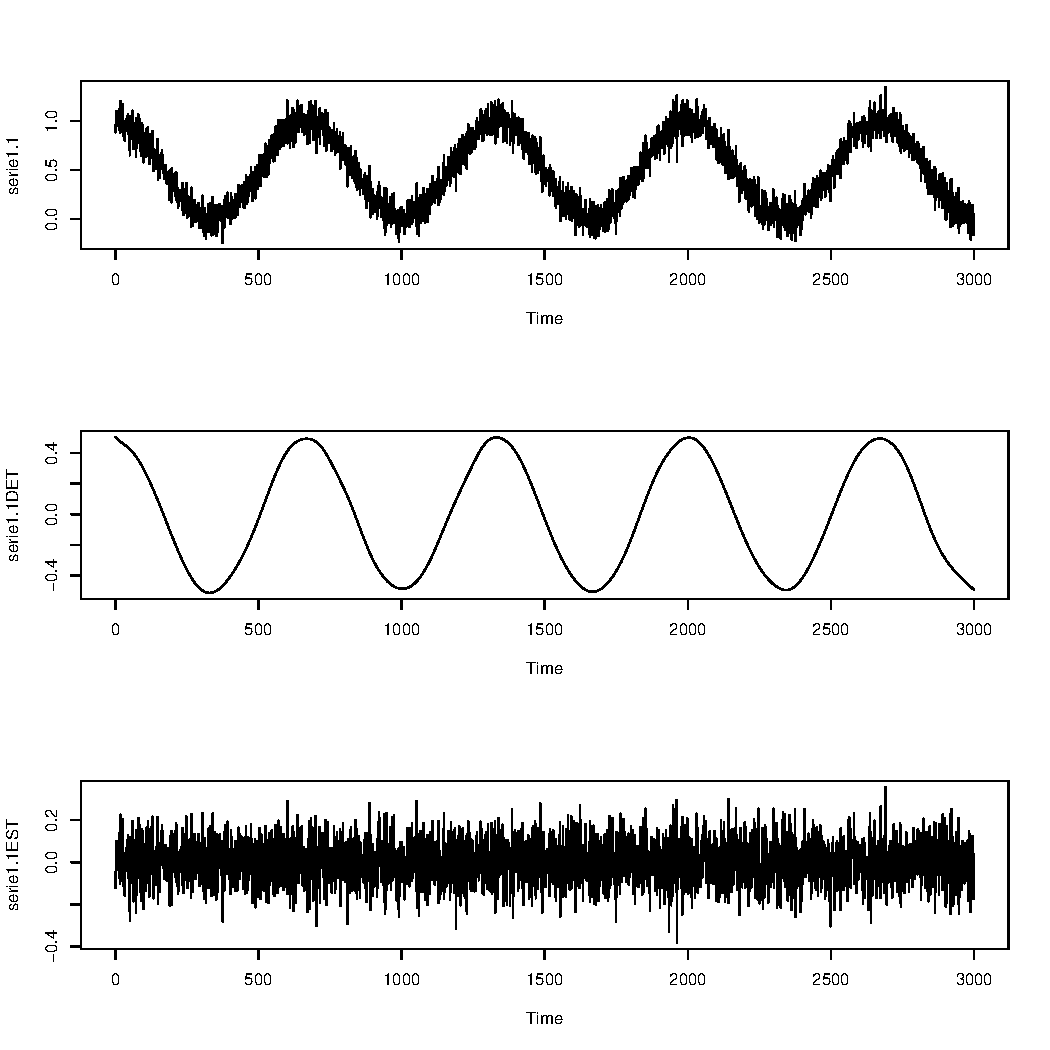
\includegraphics[scale=0.43]{serie1_1.pdf} \quad
  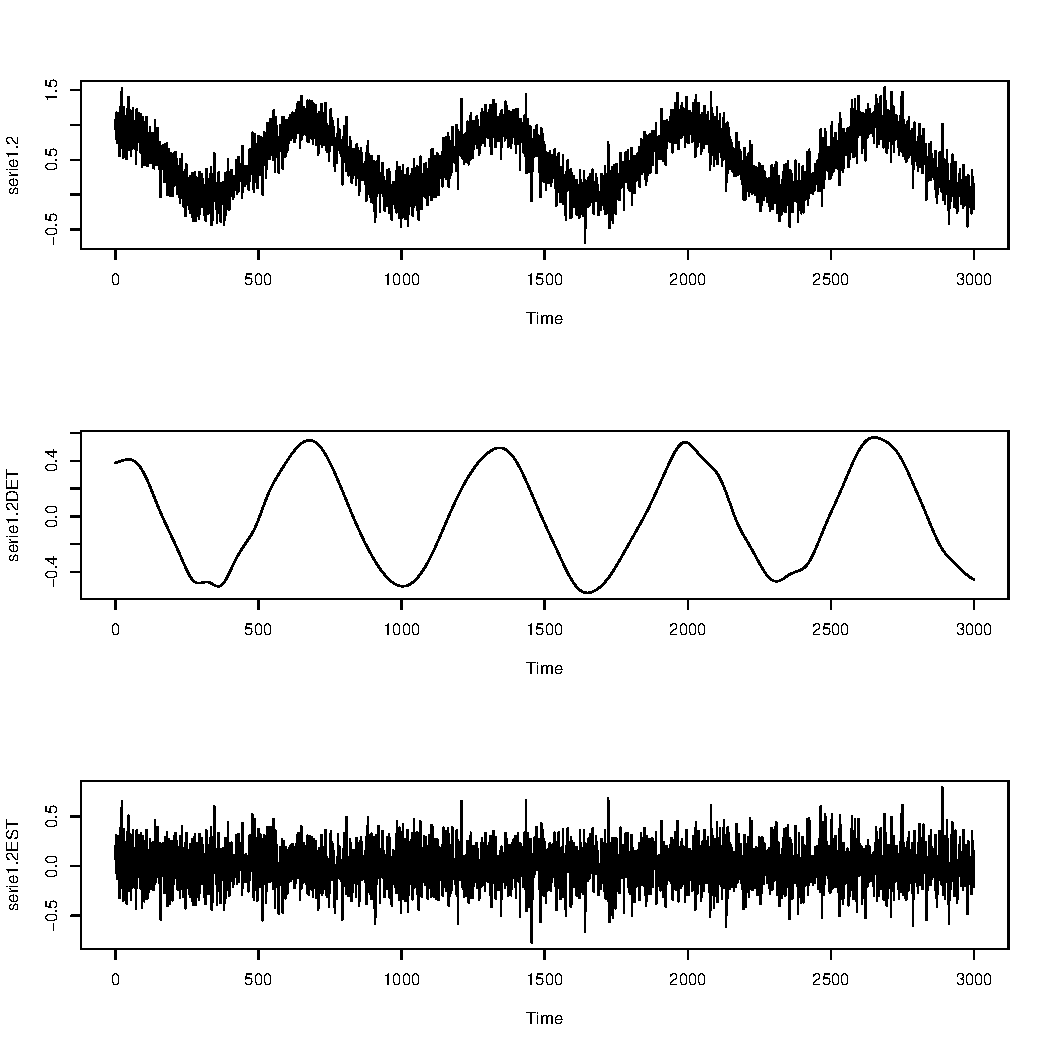
\includegraphics[scale=0.43]{serie1_2.pdf}
  \caption{Série 1.1 e Série 1.2}

\end{center}
\end{figure}

\graphicspath{{imagens/}}
\begin{figure}[H]
\begin{center}
  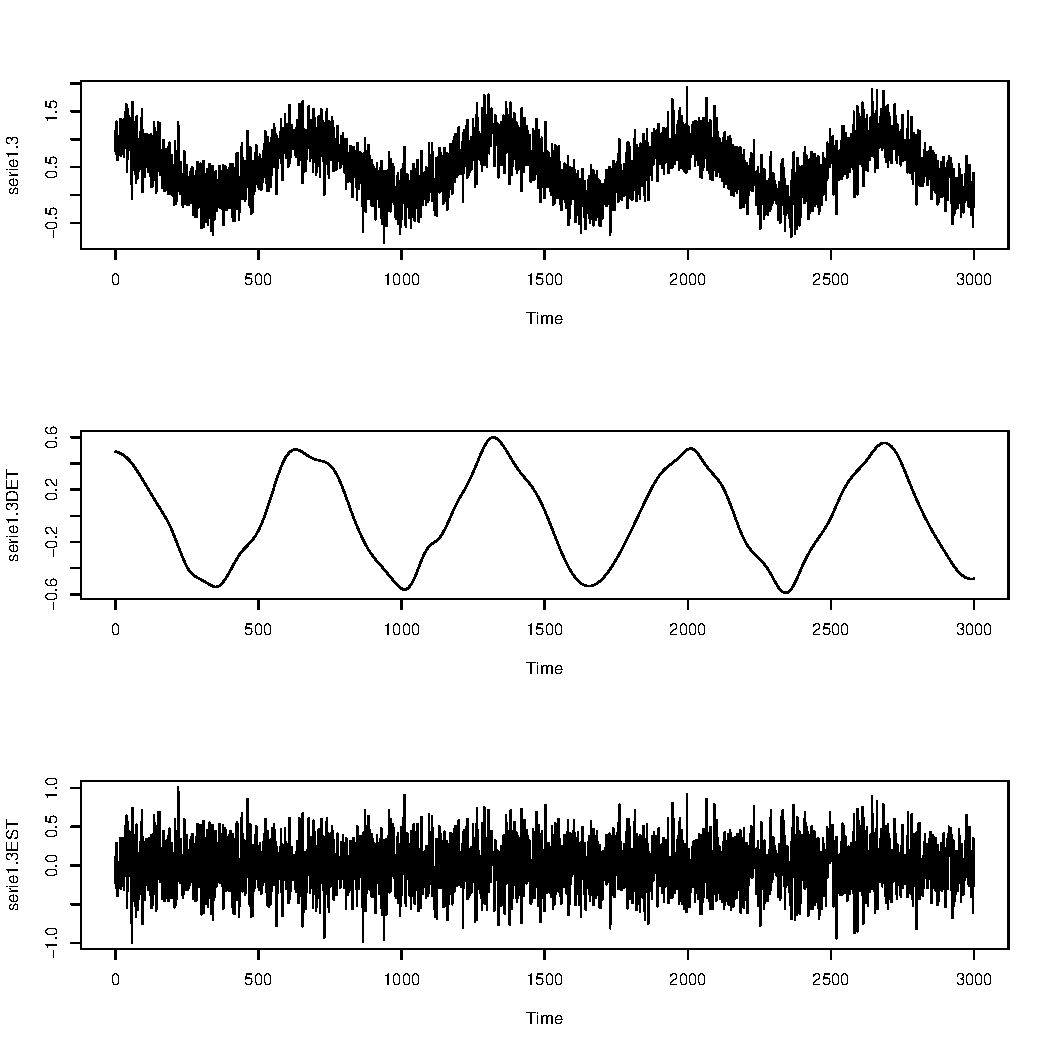
\includegraphics[scale=0.43]{serie1_3.pdf} \quad
  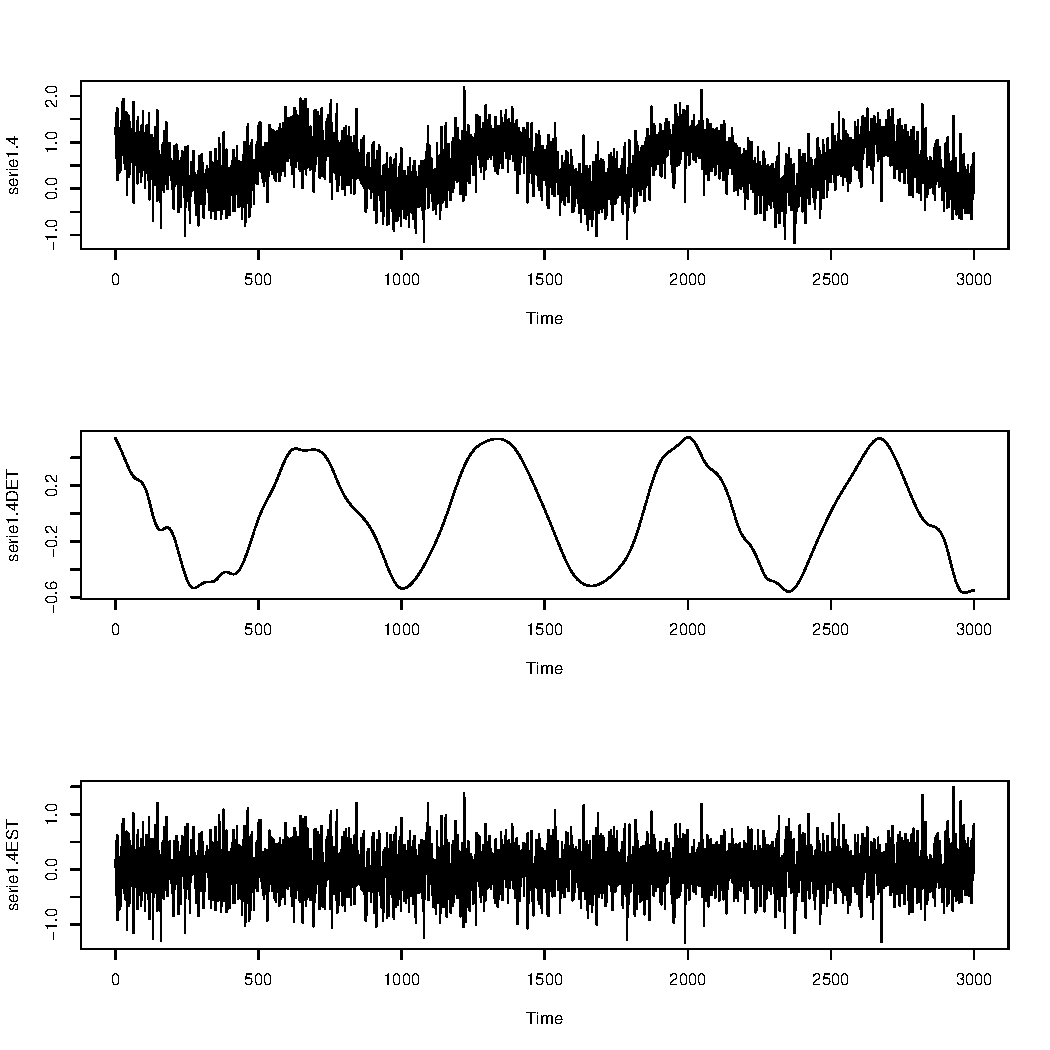
\includegraphics[scale=0.43]{serie1_4.pdf}
  \caption{Série 1.3 e Série 1.4}

\end{center}
\end{figure}

\graphicspath{{imagens/}}
\begin{figure}[H]
\begin{center}
  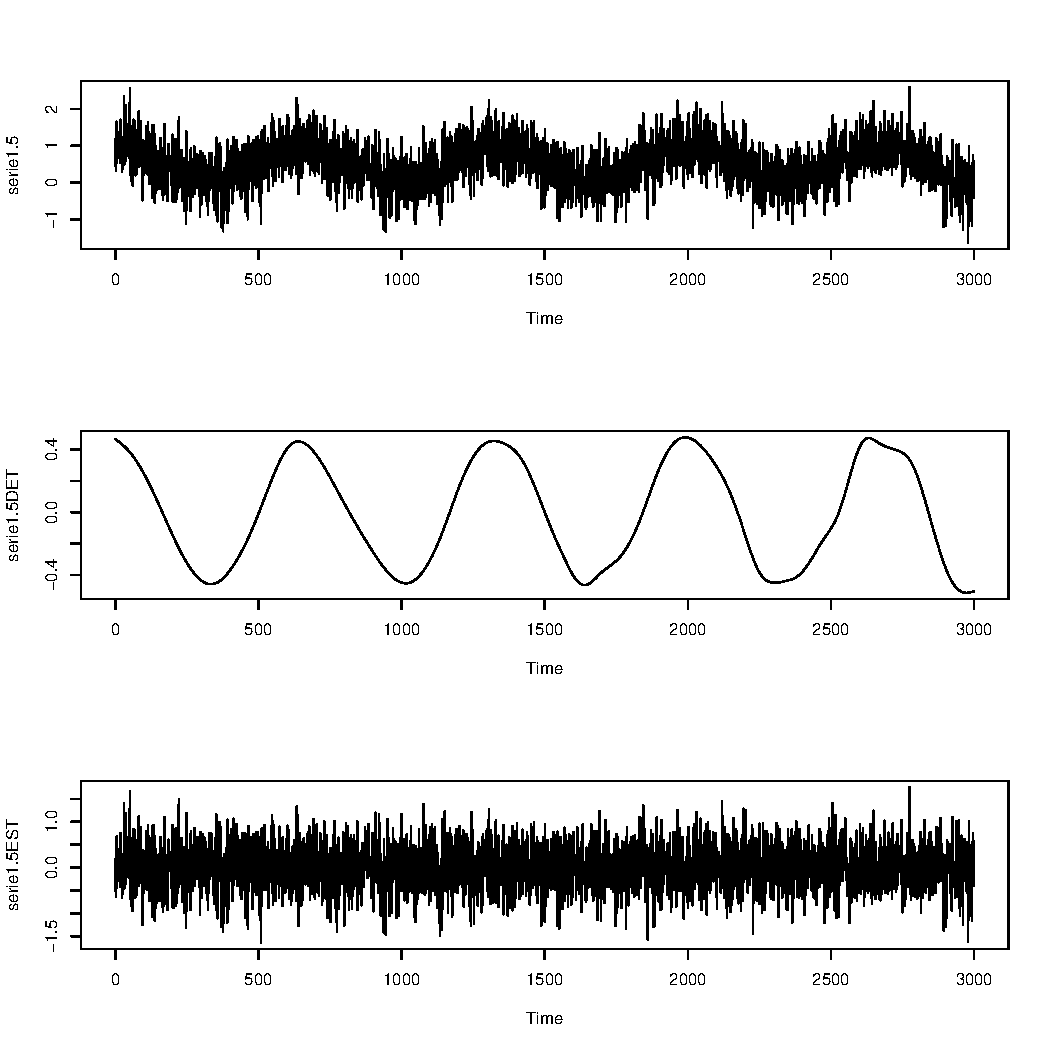
\includegraphics[scale=0.43]{serie1_5.pdf} \quad
  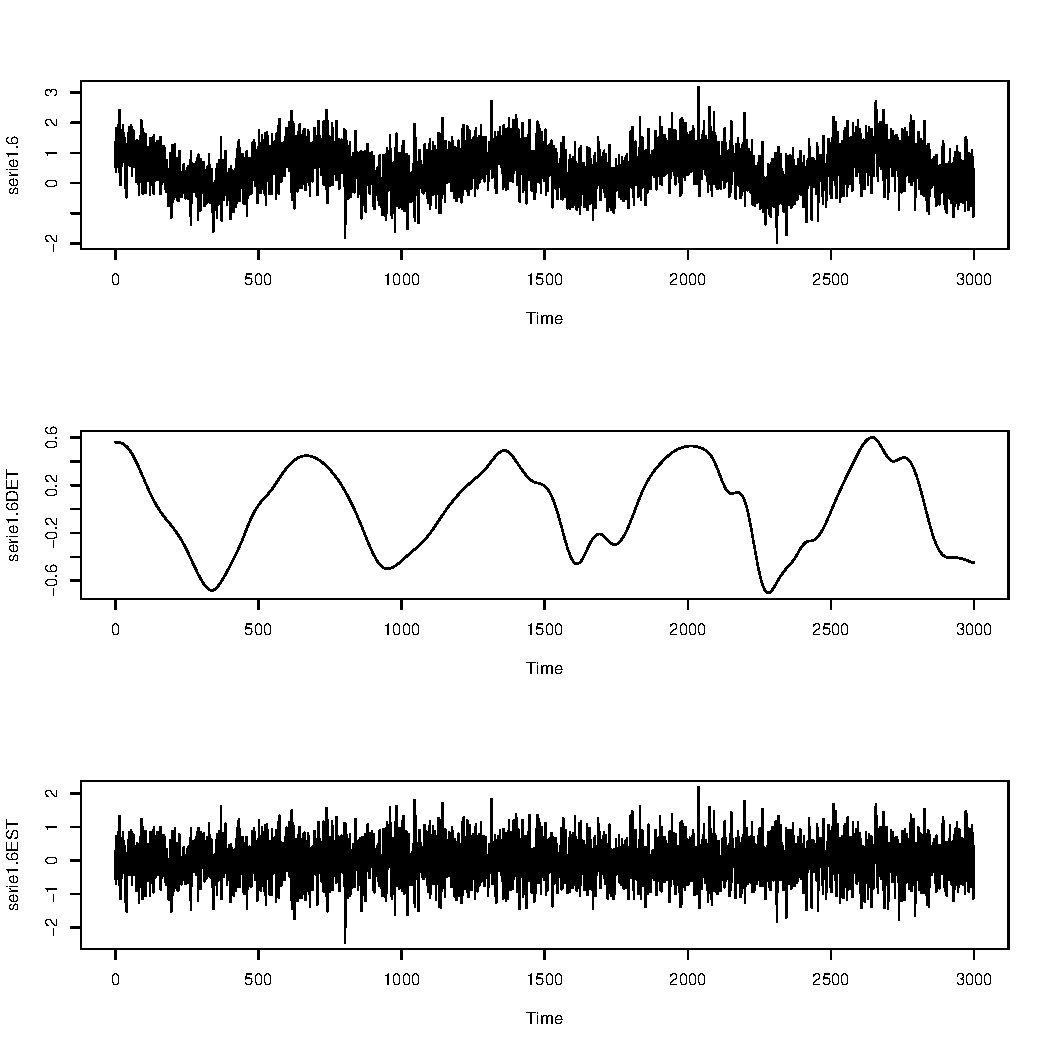
\includegraphics[scale=0.43]{serie1_6.pdf}
  \caption{Série 1.5 e Série 1.6}

\end{center}
\end{figure}

\graphicspath{{imagens/}}
\begin{figure}[H]
\begin{center}
  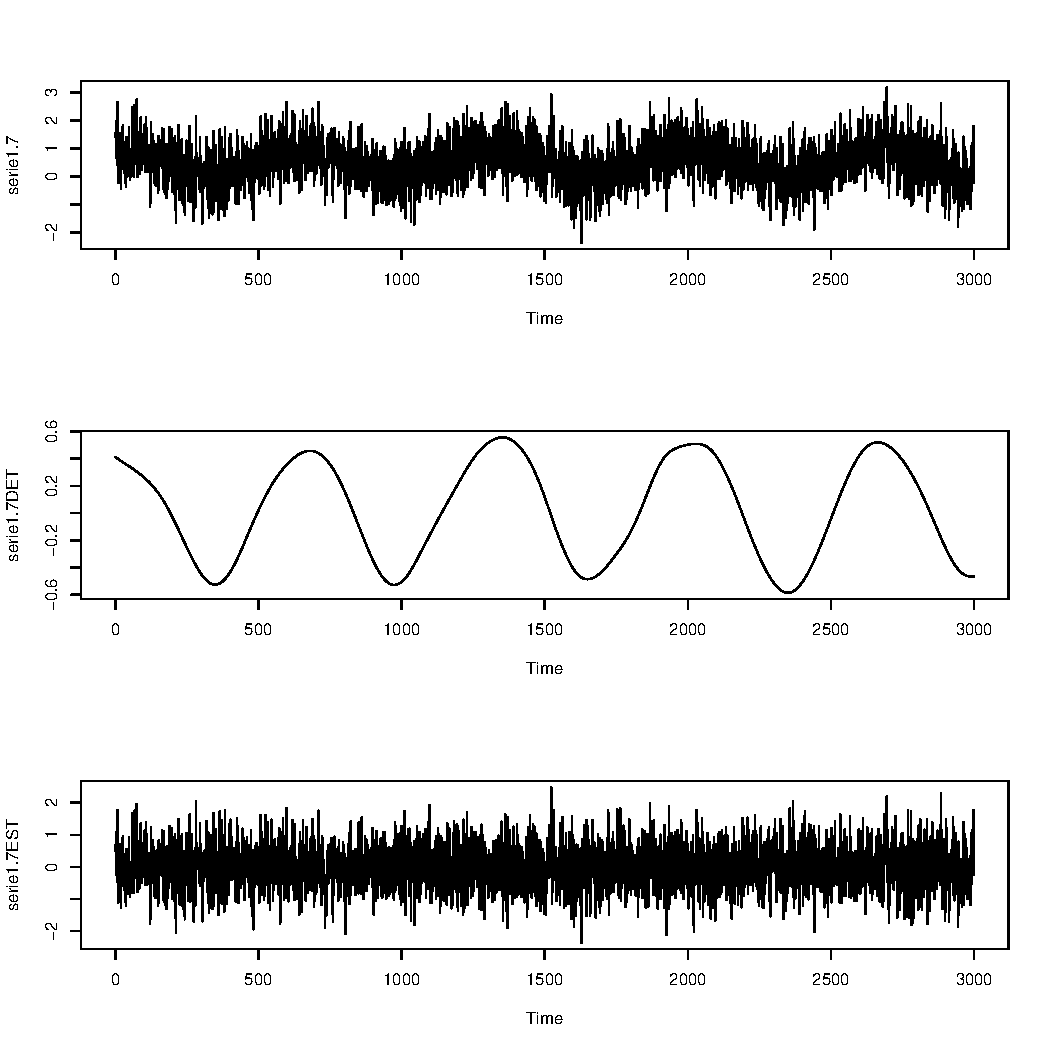
\includegraphics[scale=0.43]{serie1_7.pdf} \quad
  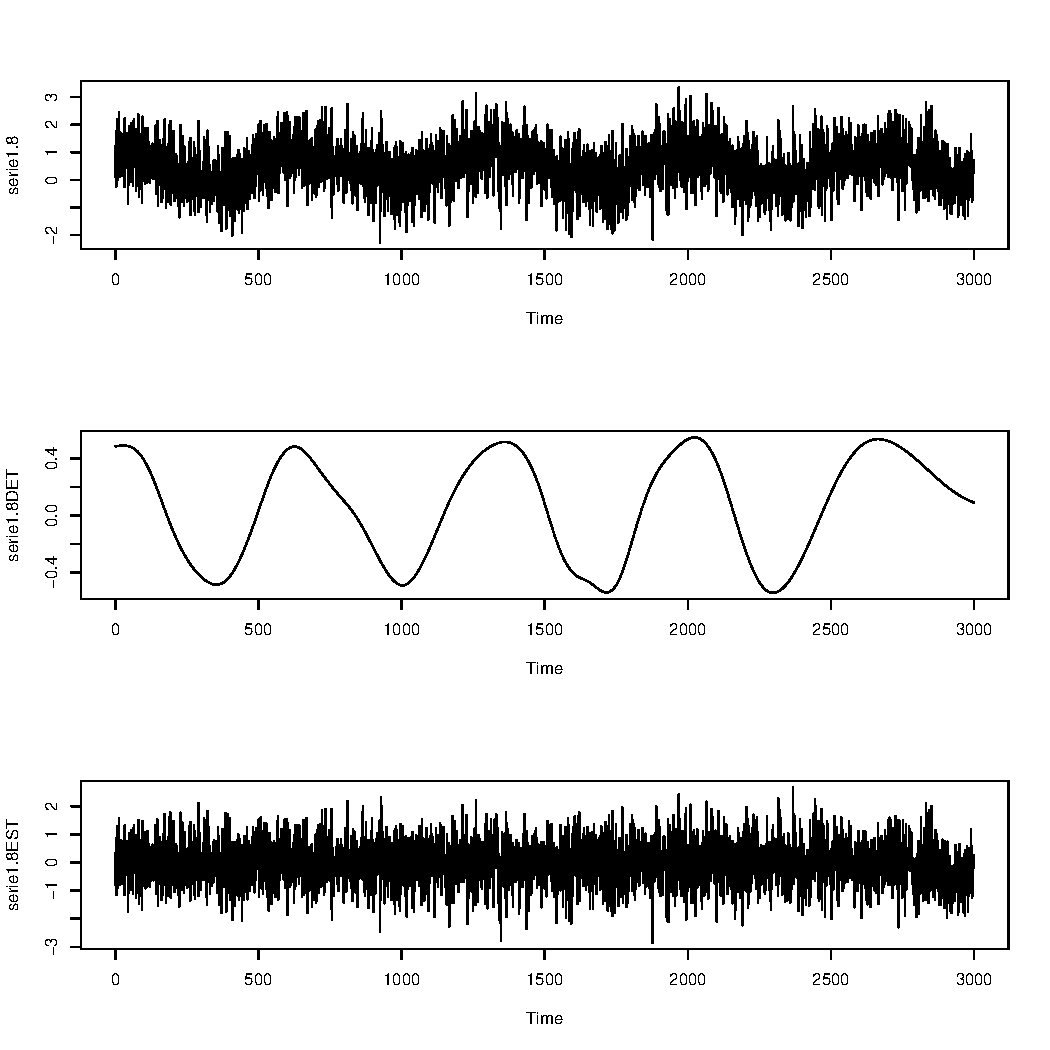
\includegraphics[scale=0.43]{serie1_8.pdf}
  \caption{Série 1.7 e Série 1.8}

\end{center}
\end{figure}

\graphicspath{{imagens/}}
\begin{figure}[H]
\begin{center}
  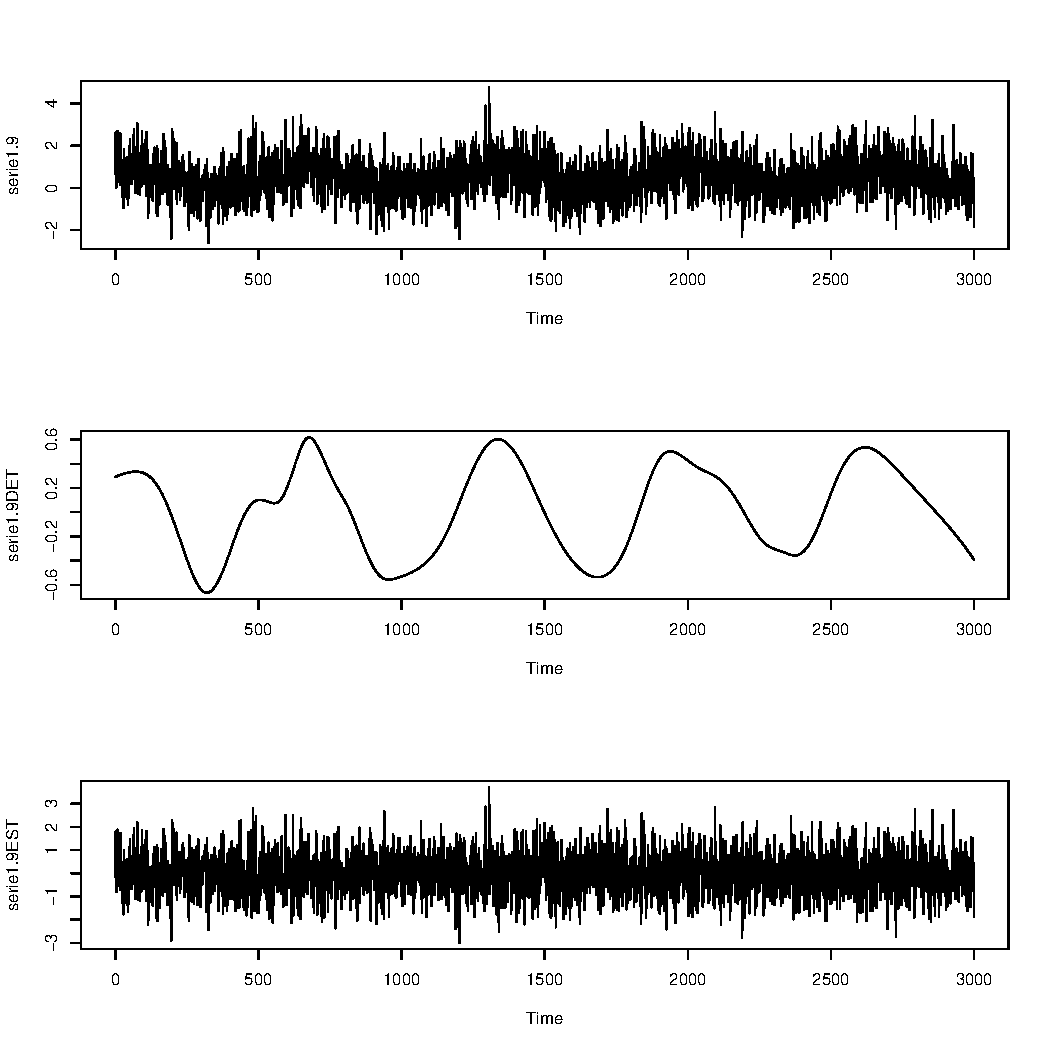
\includegraphics[scale=0.43]{serie1_9.pdf} \quad
  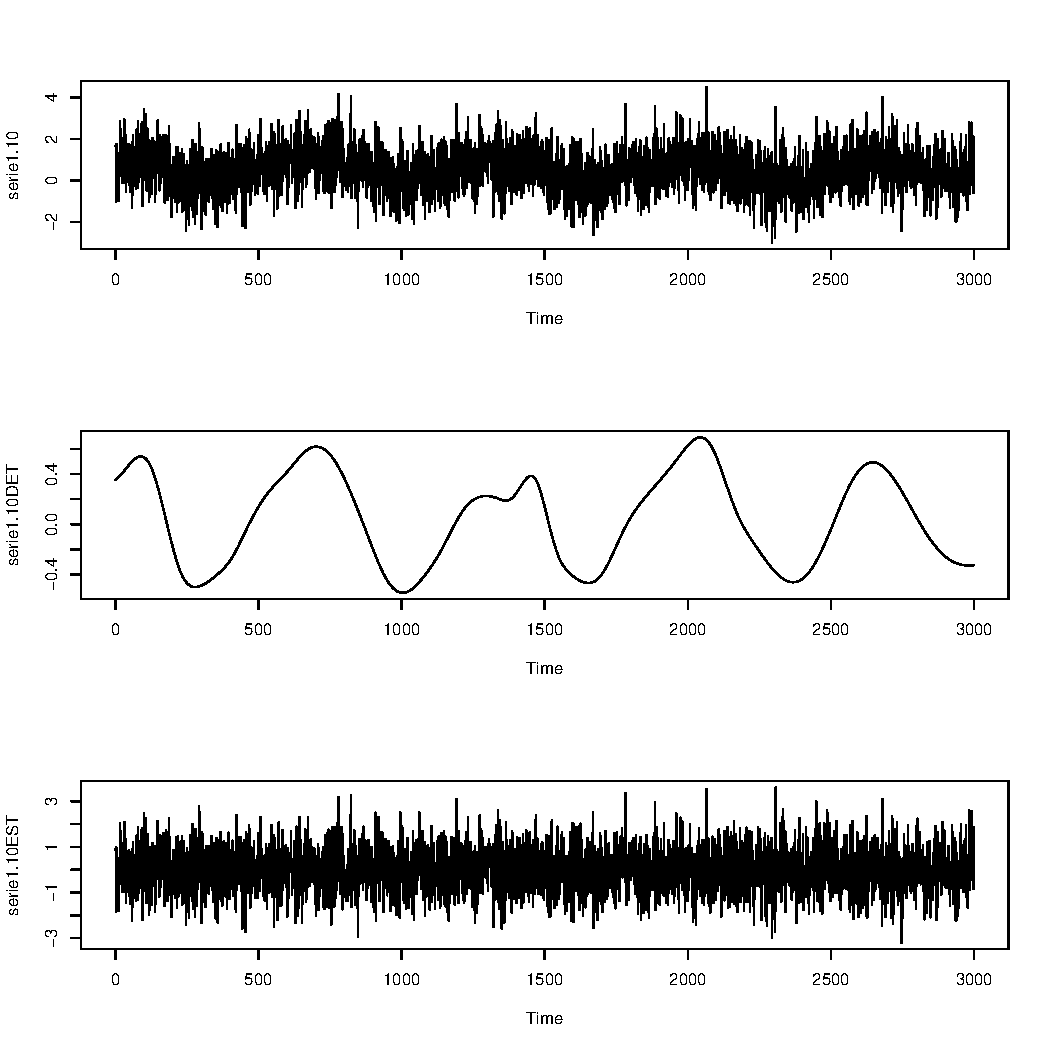
\includegraphics[scale=0.43]{serie1_10.pdf}
  \caption{Série 1.9 e Série 1.10}

\end{center}
\end{figure}

\section{Séries TIPO 2}
10 séries cossenoide com ruído ao longo da série e tendência.
\graphicspath{{imagens/}}
\begin{figure}[H]
\begin{center}
  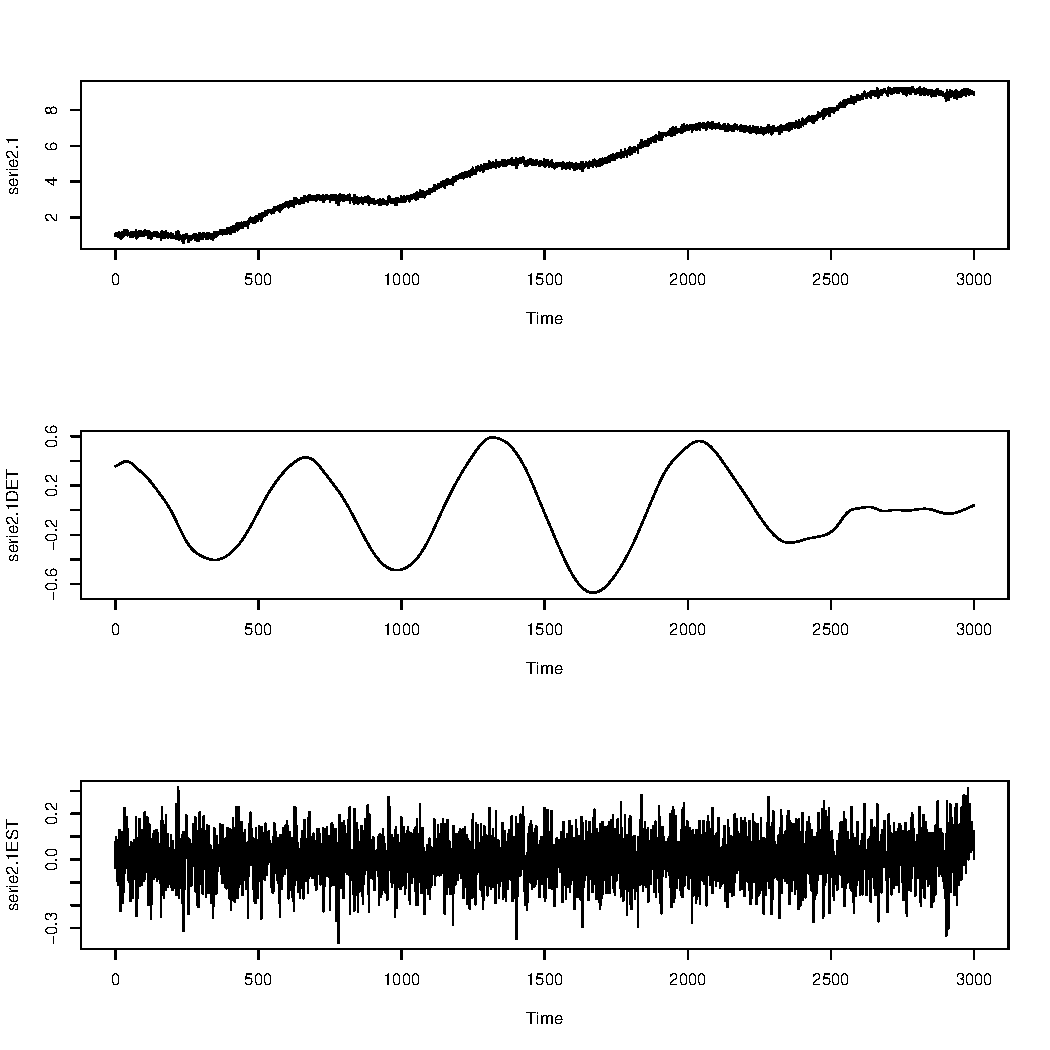
\includegraphics[scale=0.43]{serie2_1.pdf} \quad
  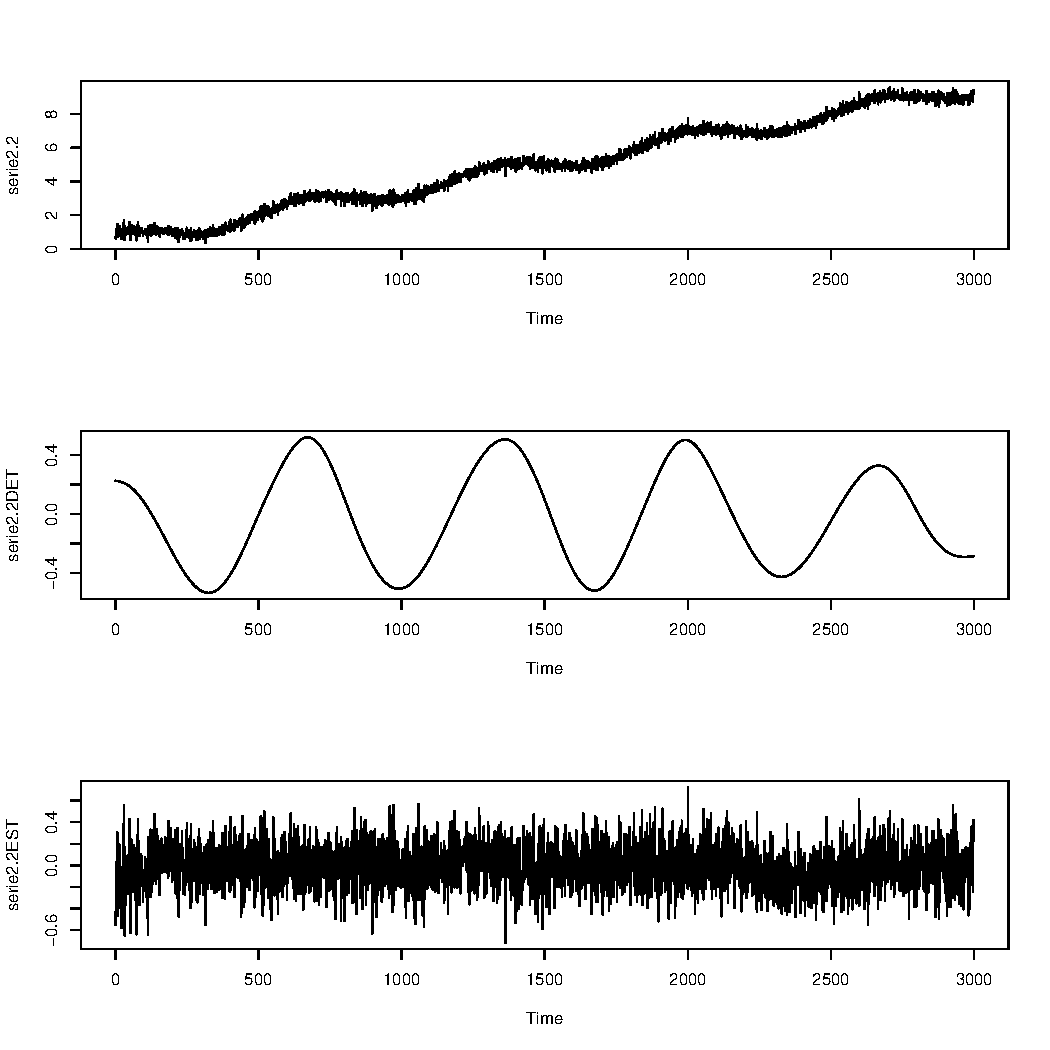
\includegraphics[scale=0.43]{serie2_2.pdf}
  \caption{Série 2.1 e Série 2.2}

\end{center}
\end{figure}

\graphicspath{{imagens/}}
\begin{figure}[H]
\begin{center}
  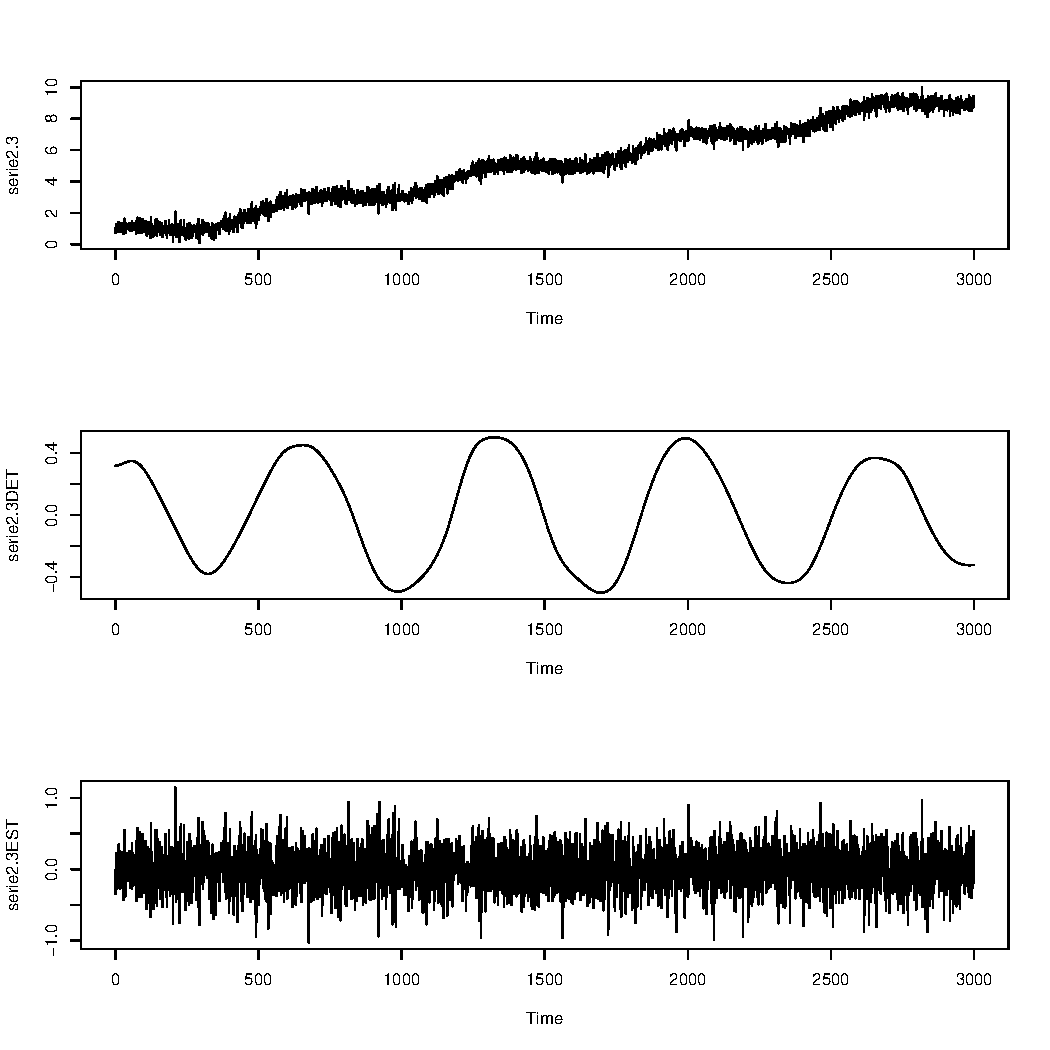
\includegraphics[scale=0.43]{serie2_3.pdf} \quad
  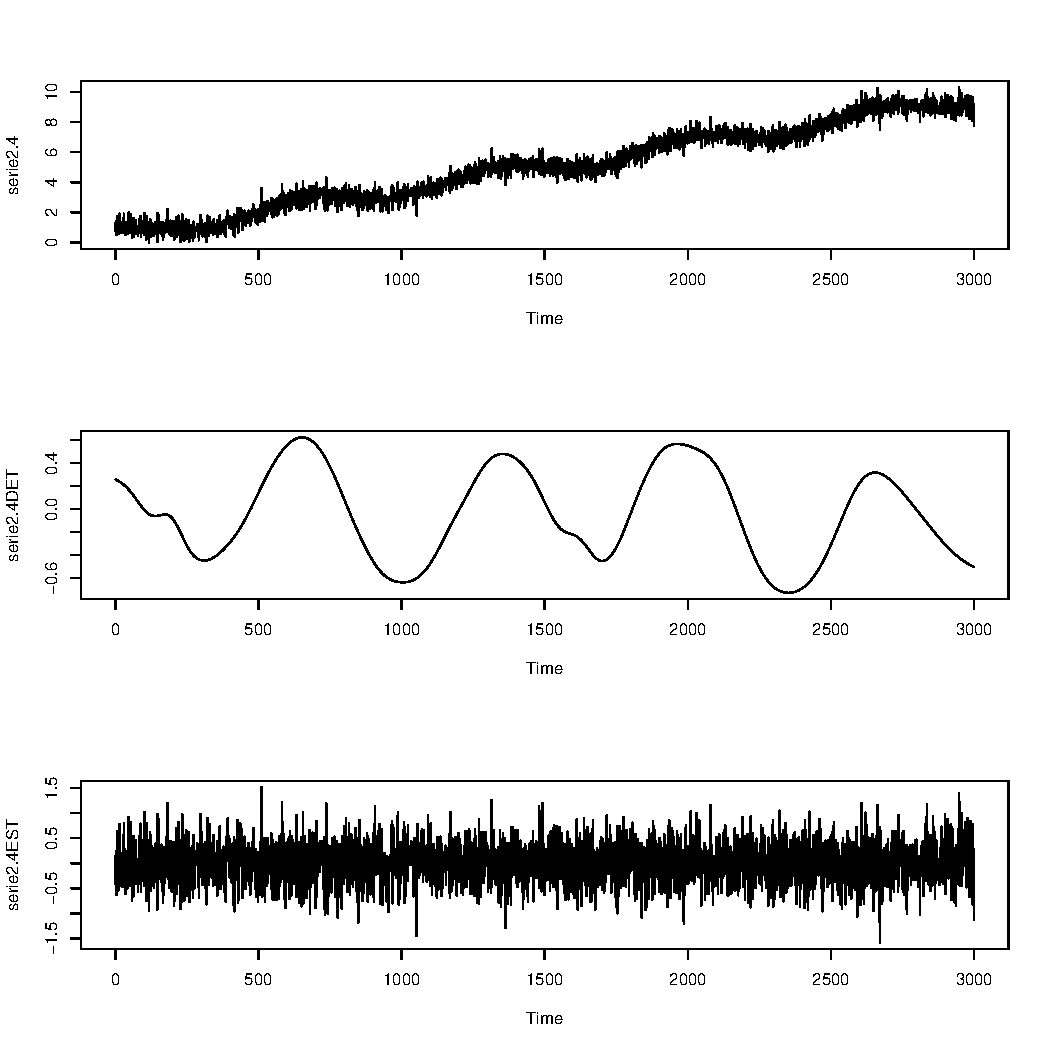
\includegraphics[scale=0.43]{serie2_4.pdf}
  \caption{Série 2.3 e Série 2.4}

\end{center}
\end{figure}

\graphicspath{{imagens/}}
\begin{figure}[H]
\begin{center}
  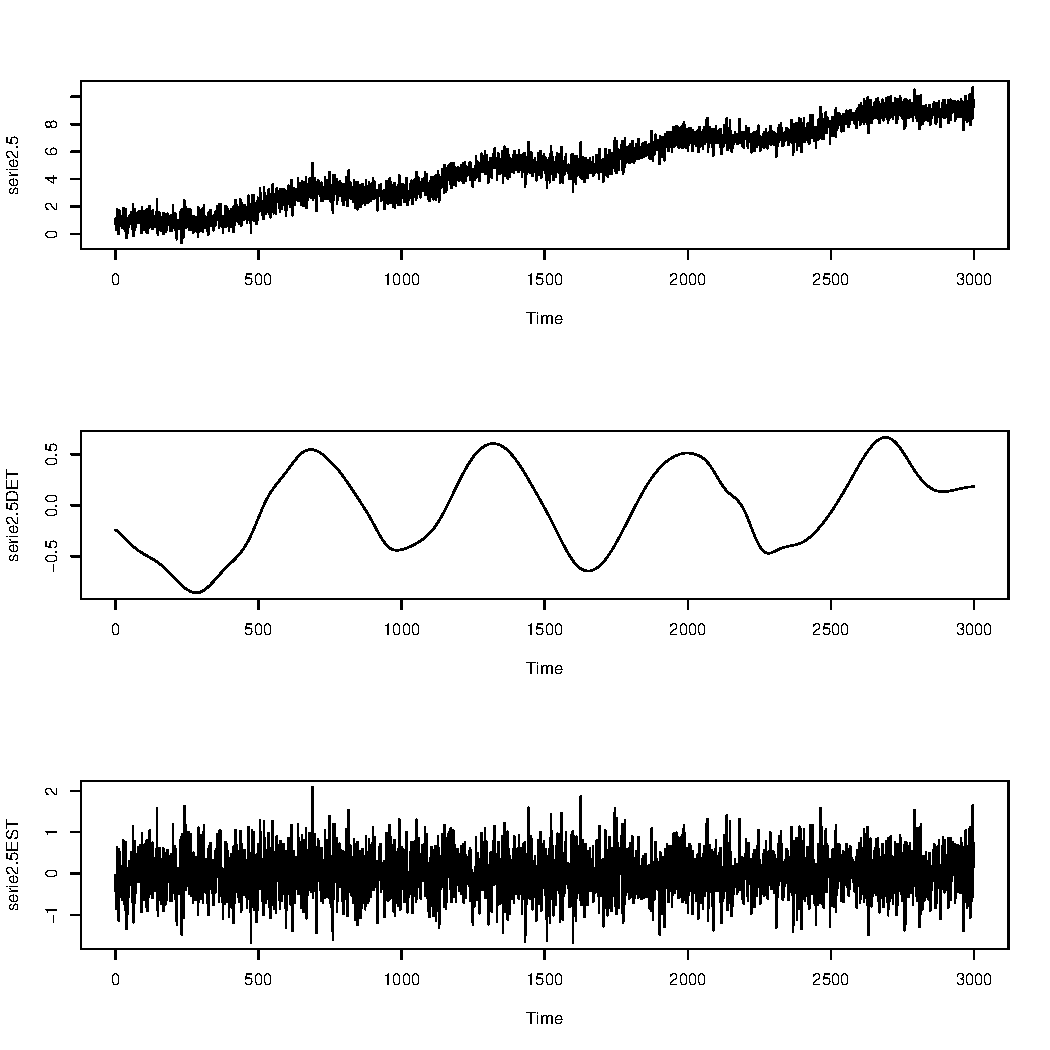
\includegraphics[scale=0.43]{serie2_5.pdf} \quad
  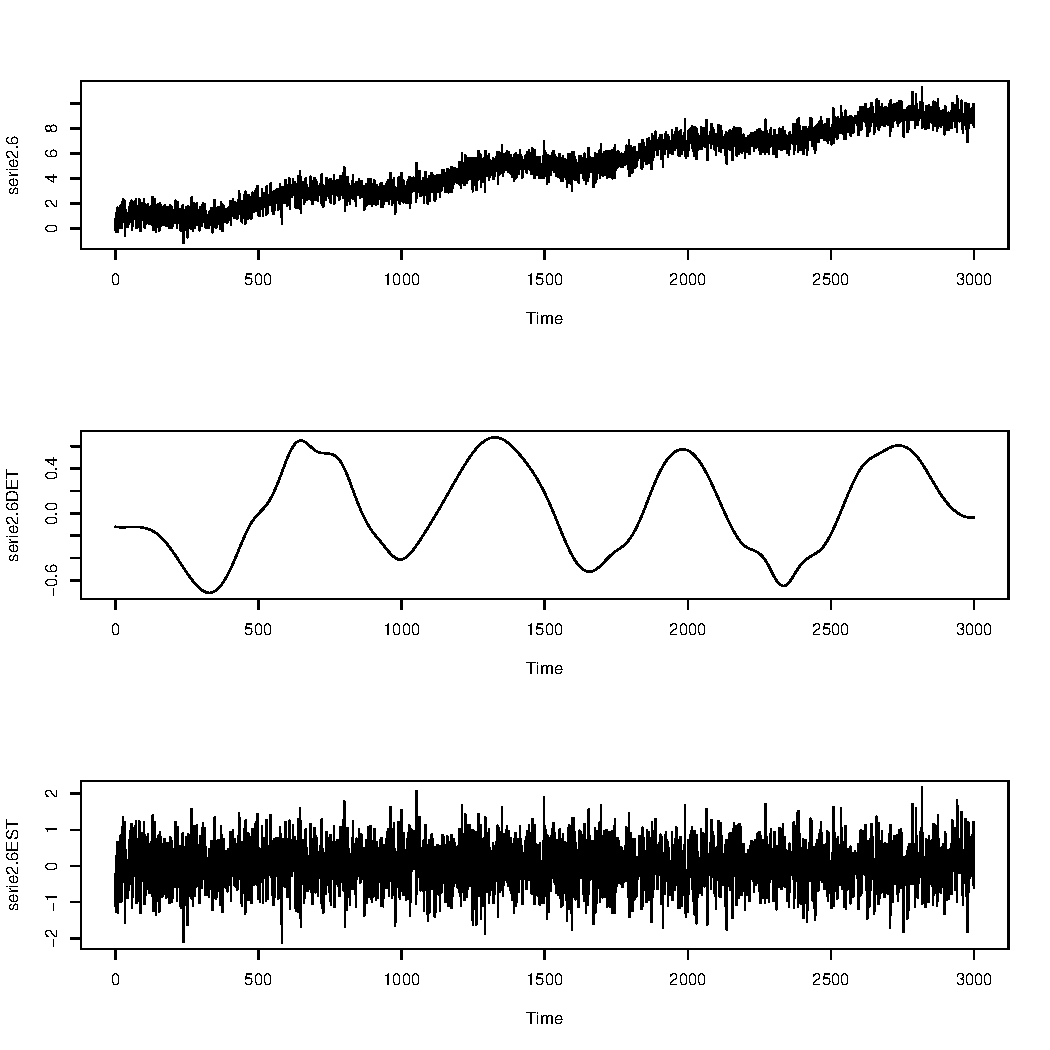
\includegraphics[scale=0.43]{serie2_6.pdf}
  \caption{Série 2.5 e Série 2.6}

\end{center}
\end{figure}

\graphicspath{{imagens/}}
\begin{figure}[H]
\begin{center}
  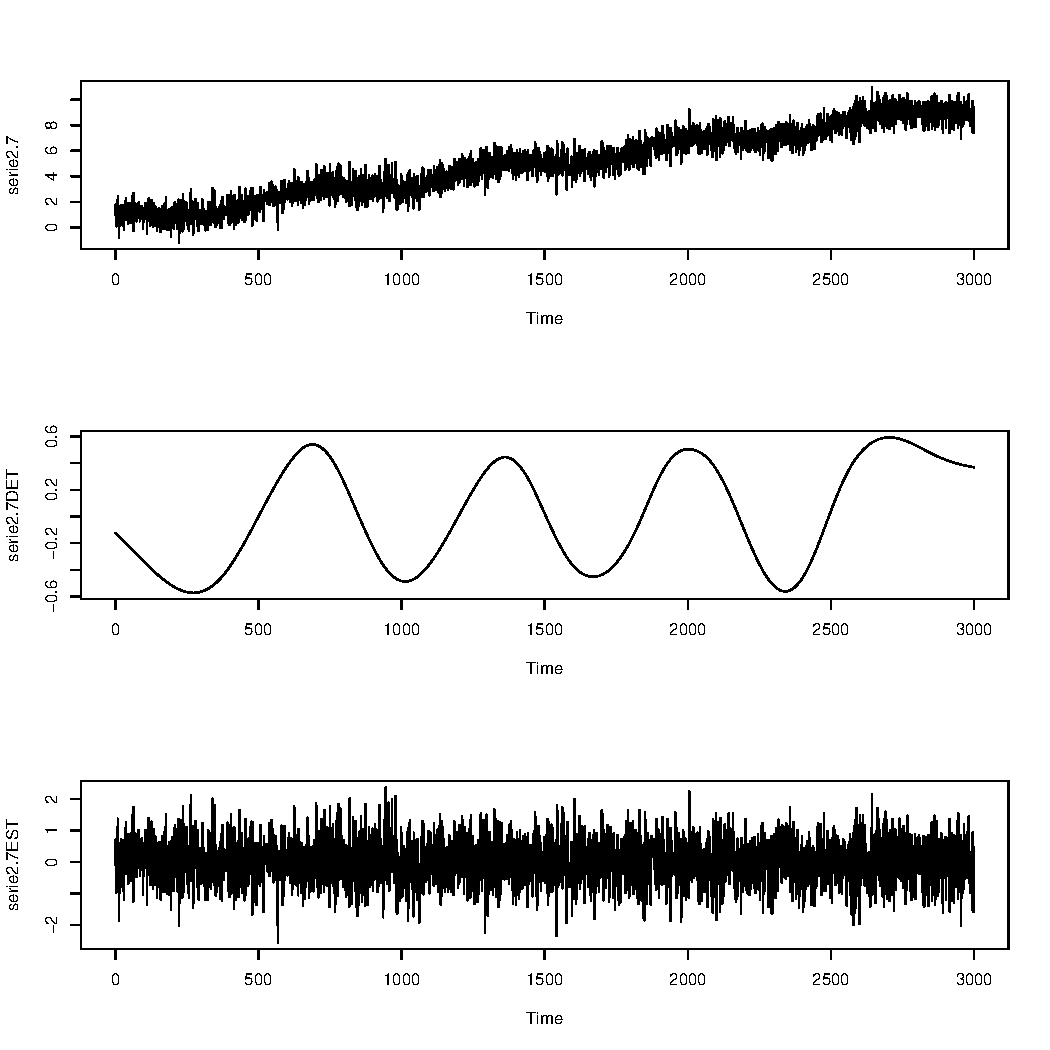
\includegraphics[scale=0.43]{serie2_7.pdf} \quad
  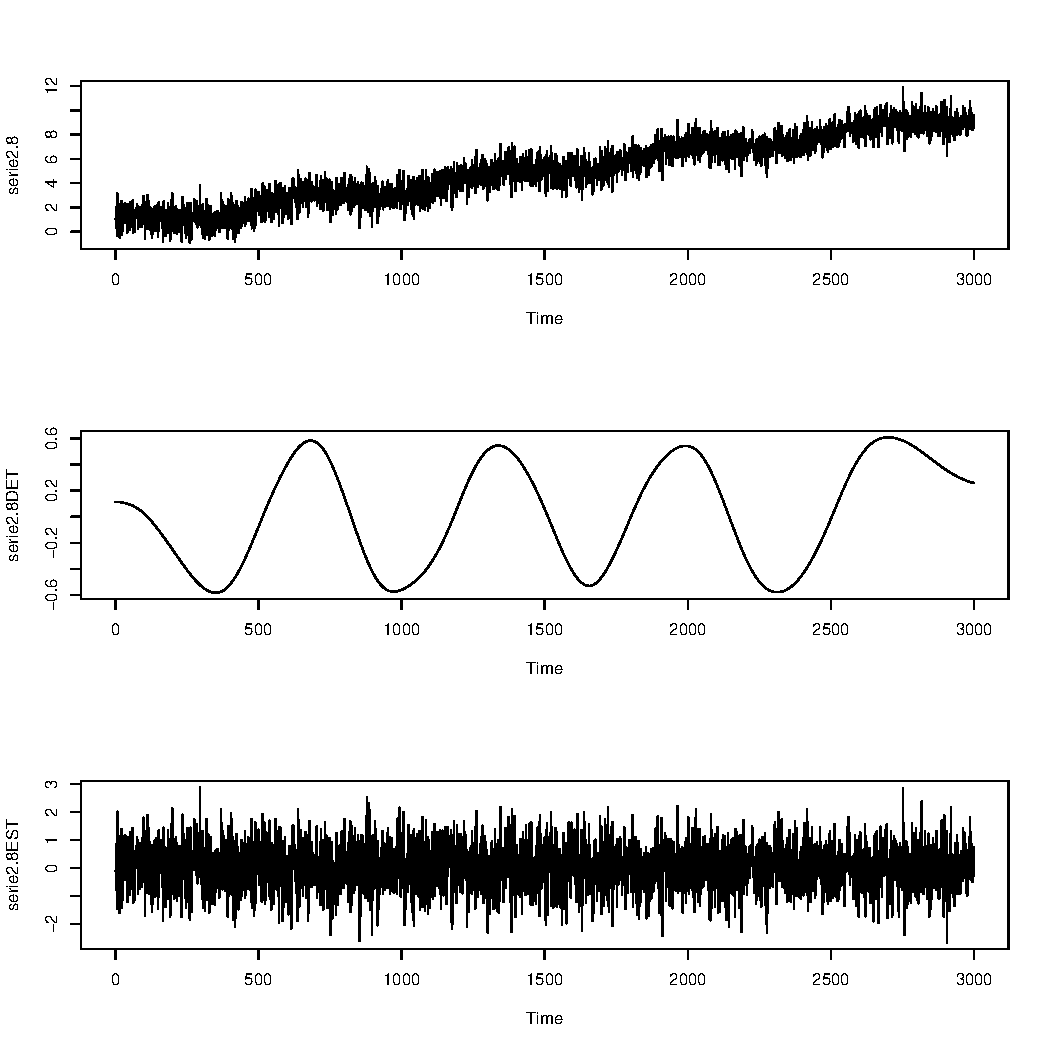
\includegraphics[scale=0.43]{serie2_8.pdf}
  \caption{Série 2.7 e Série 2.8}

\end{center}
\end{figure}

\graphicspath{{imagens/}}
\begin{figure}[H]
\begin{center}
  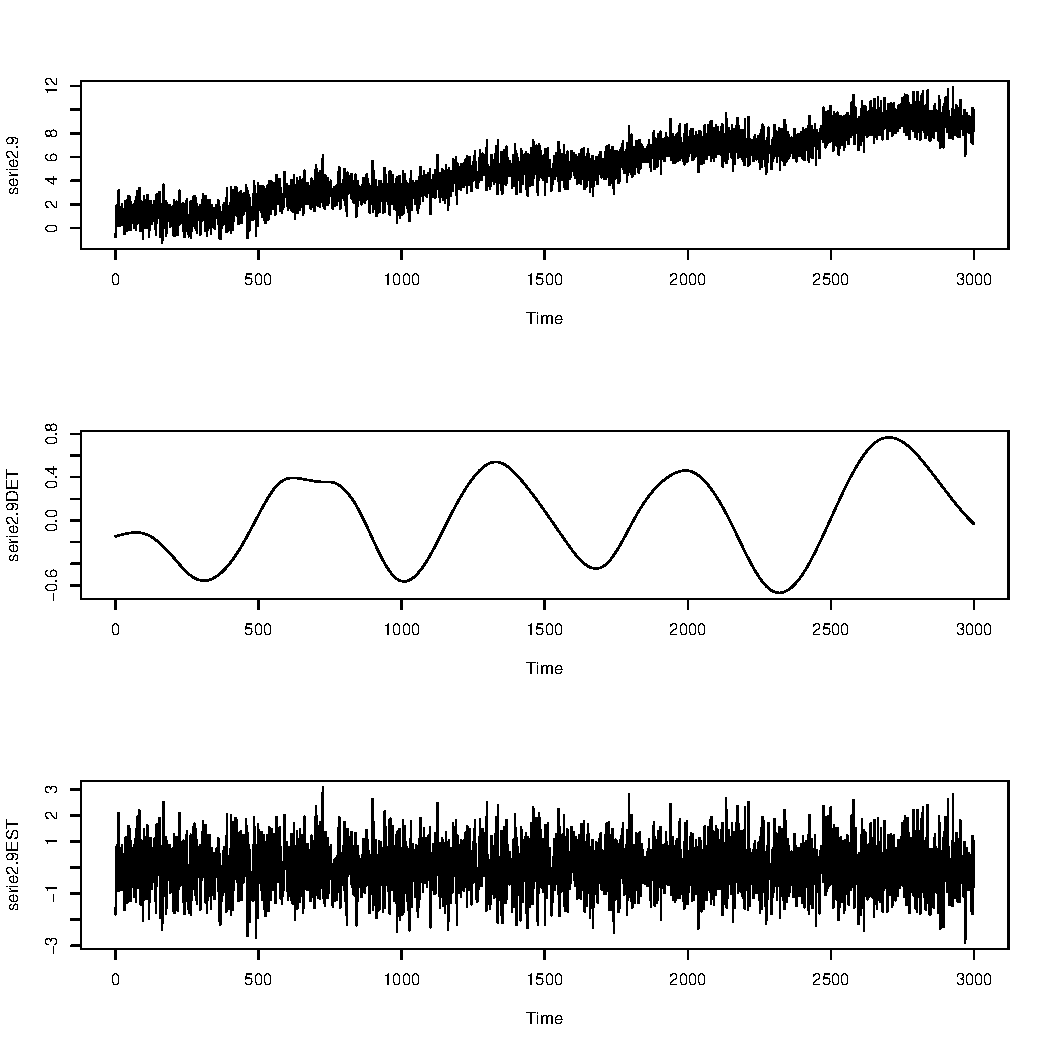
\includegraphics[scale=0.43]{serie2_9.pdf} \quad
  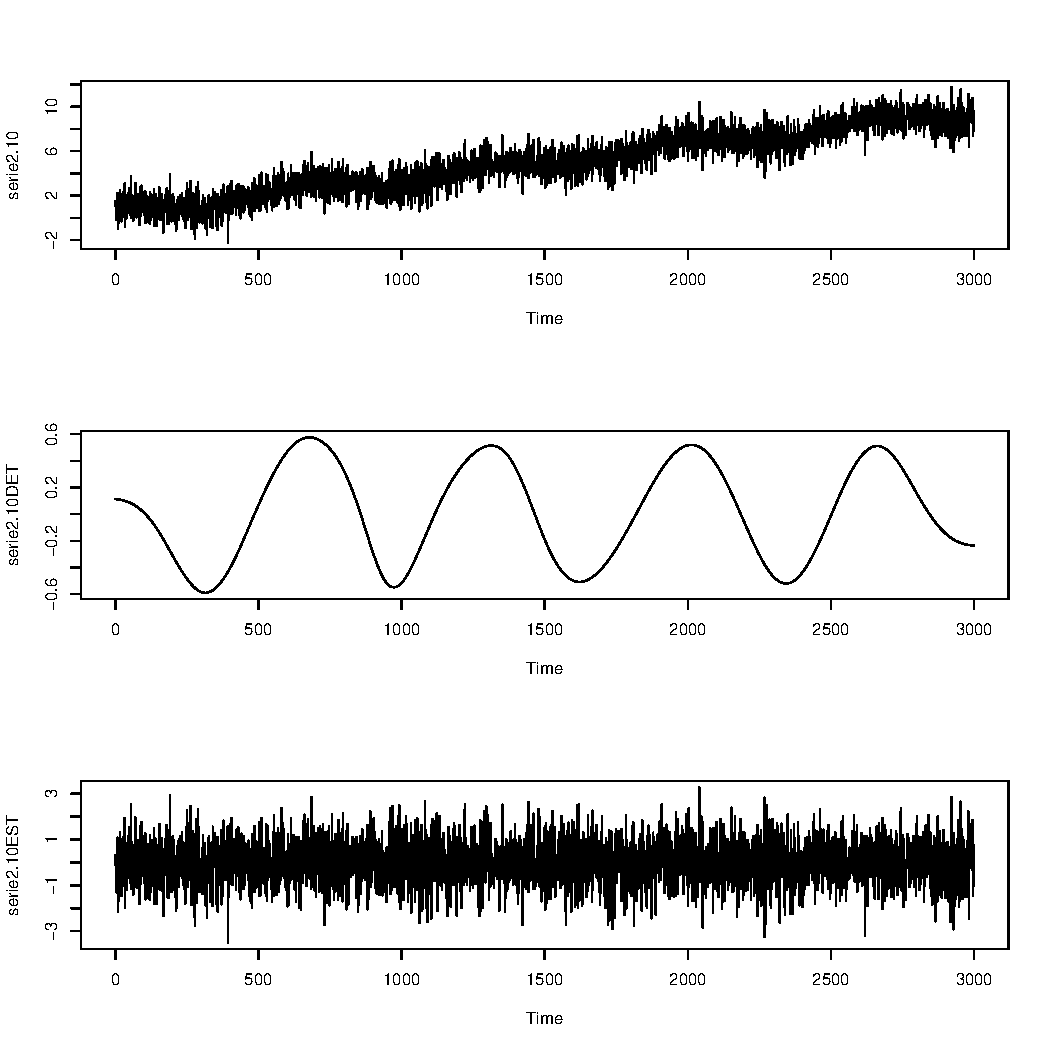
\includegraphics[scale=0.43]{serie2_10.pdf}
  \caption{Série 2.9 e Série 2.10}

\end{center}
\end{figure}

\section{Séries TIPO 3}
10 séries senoide com ruído ao longo da série.
\graphicspath{{imagens/}}
\begin{figure}[H]
\begin{center}
  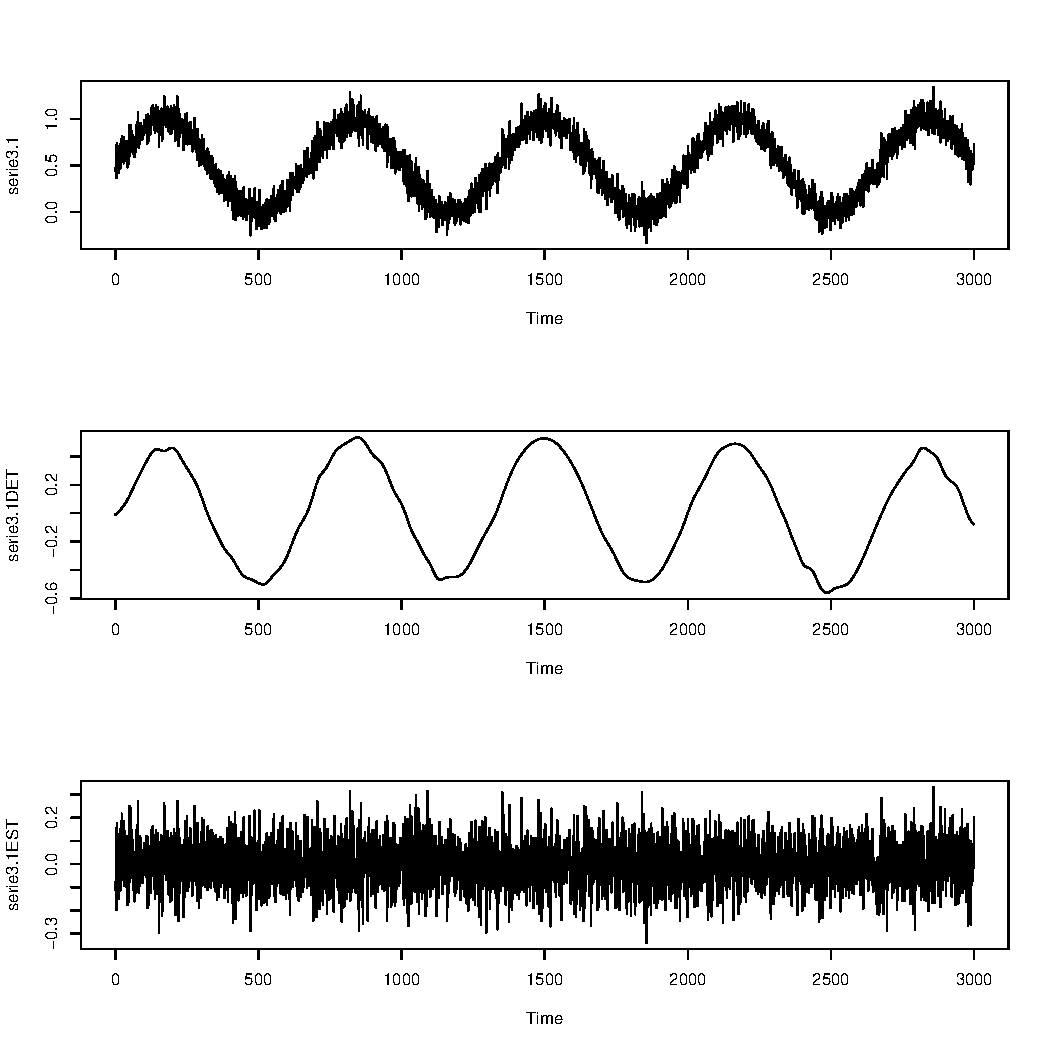
\includegraphics[scale=0.43]{serie3_1.pdf} \quad
  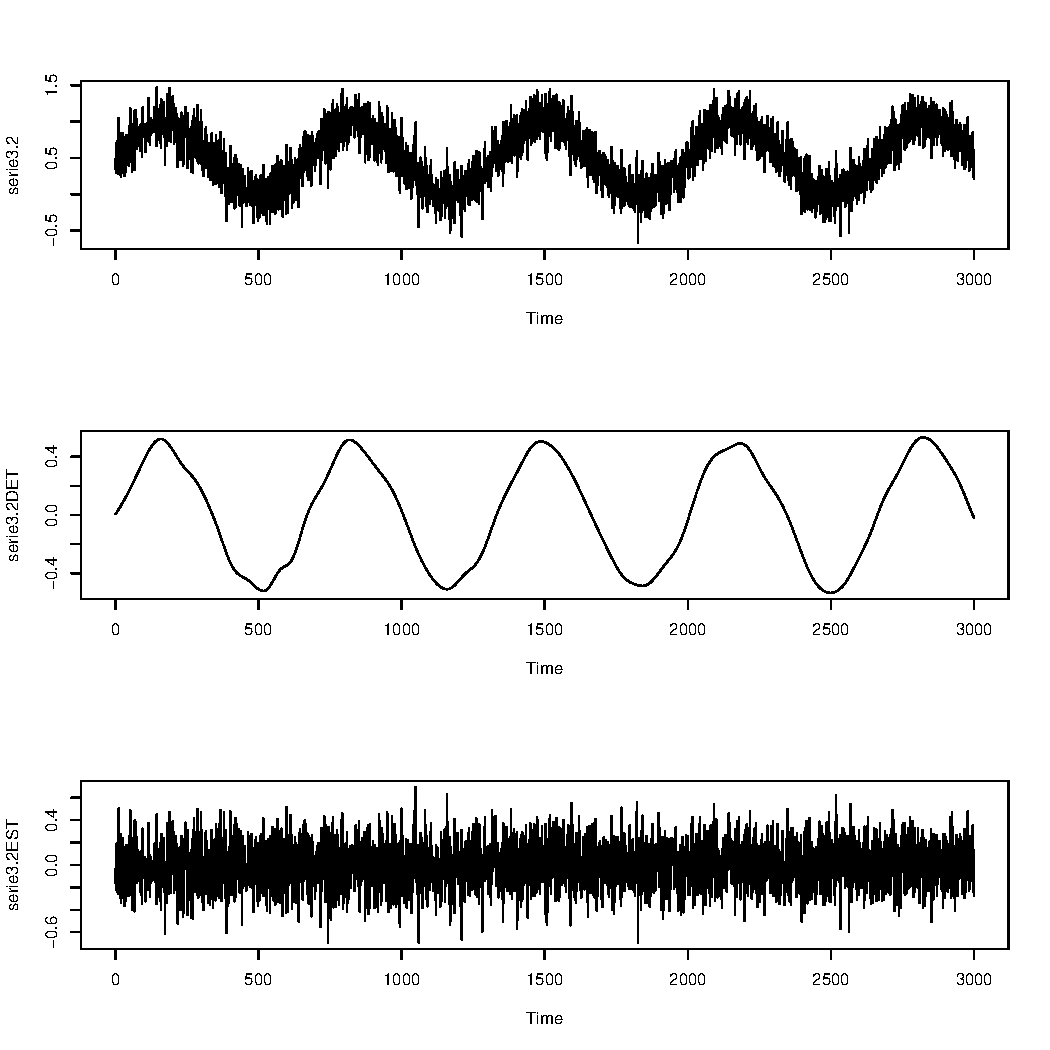
\includegraphics[scale=0.43]{serie3_2.pdf}
  \caption{Série 3.1 e Série 3.2}

\end{center}
\end{figure}

\graphicspath{{imagens/}}
\begin{figure}[H]
\begin{center}
  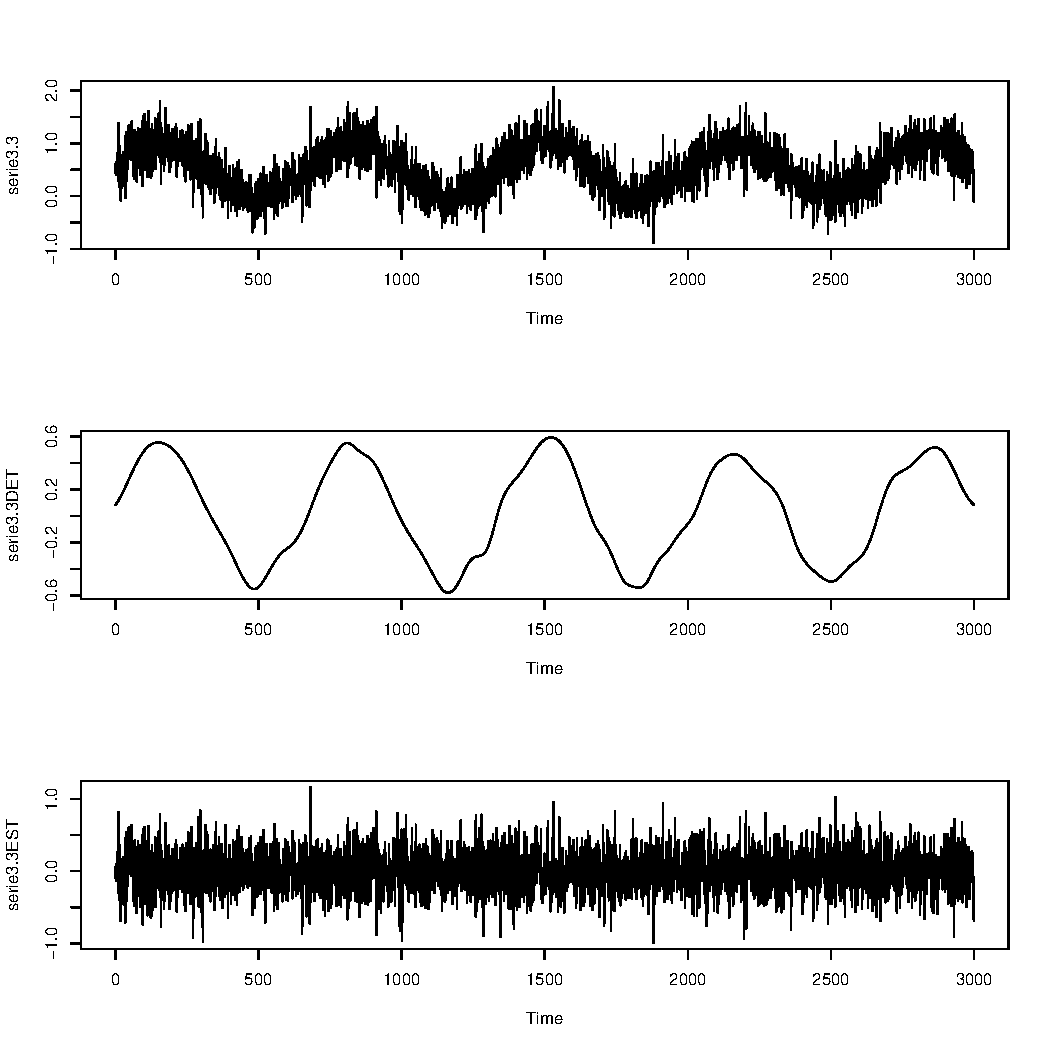
\includegraphics[scale=0.43]{serie3_3.pdf} \quad
  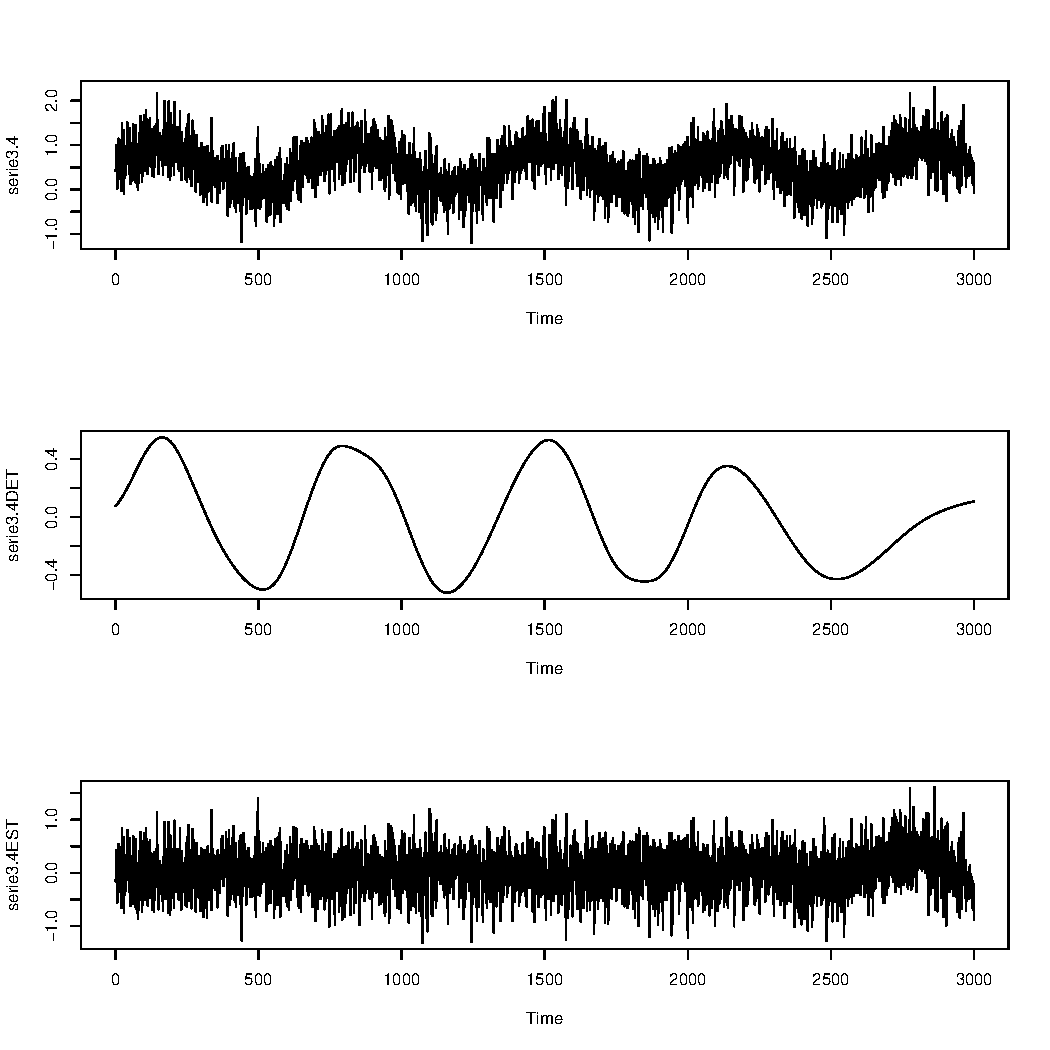
\includegraphics[scale=0.43]{serie3_4.pdf}
  \caption{Série 3.3 e Série 3.4}

\end{center}
\end{figure}

\graphicspath{{imagens/}}
\begin{figure}[H]
\begin{center}
  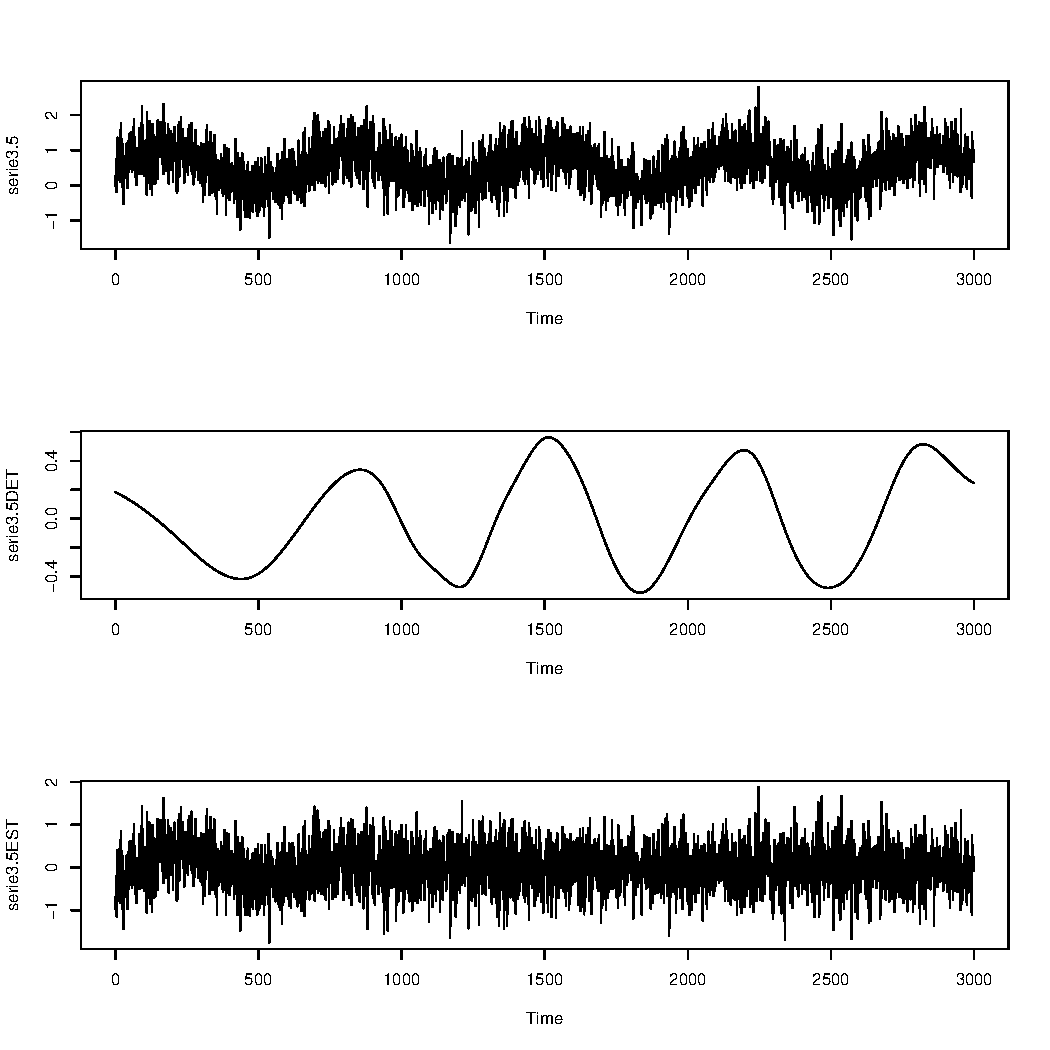
\includegraphics[scale=0.43]{serie3_5.pdf} \quad
  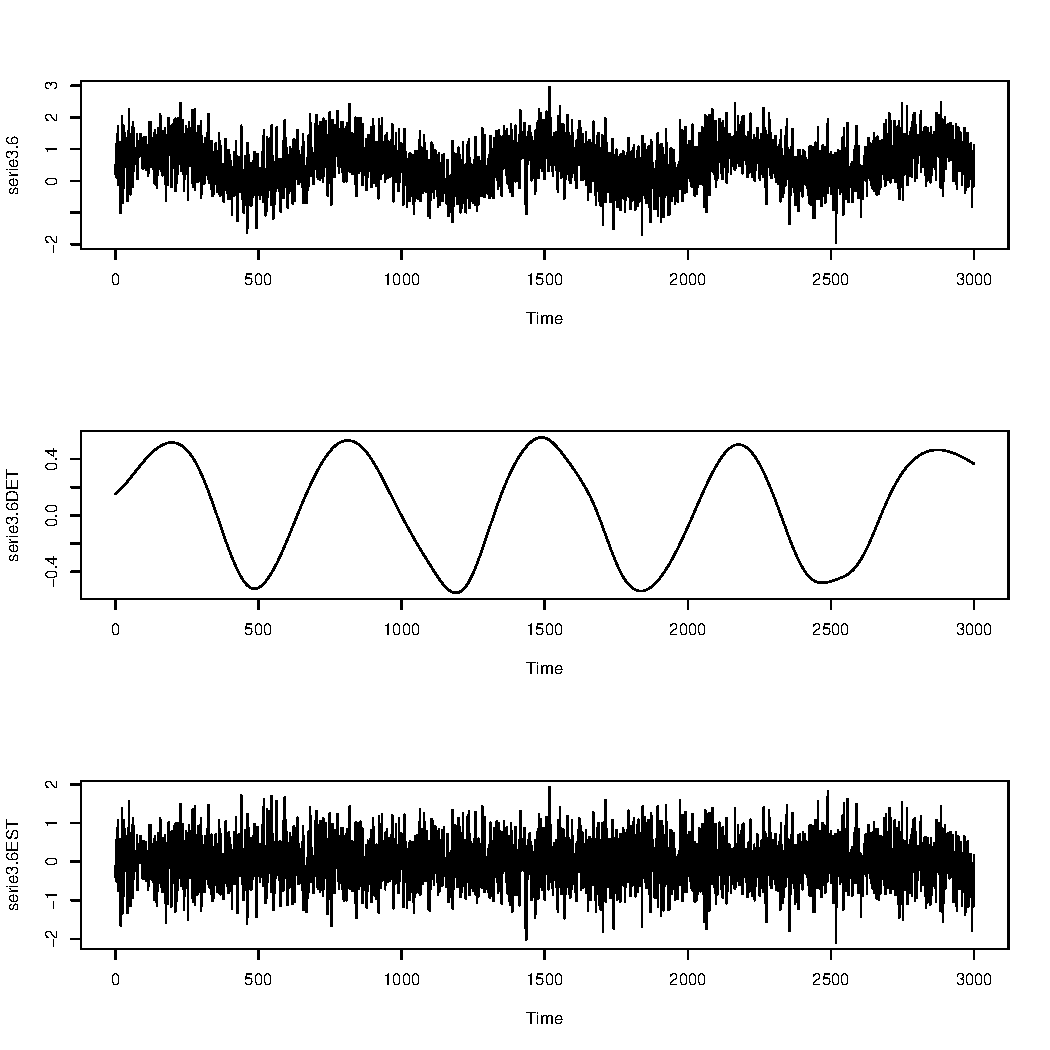
\includegraphics[scale=0.43]{serie3_6.pdf}
  \caption{Série 3.5 e Série 3.6}

\end{center}
\end{figure}

\graphicspath{{imagens/}}
\begin{figure}[H]
\begin{center}
  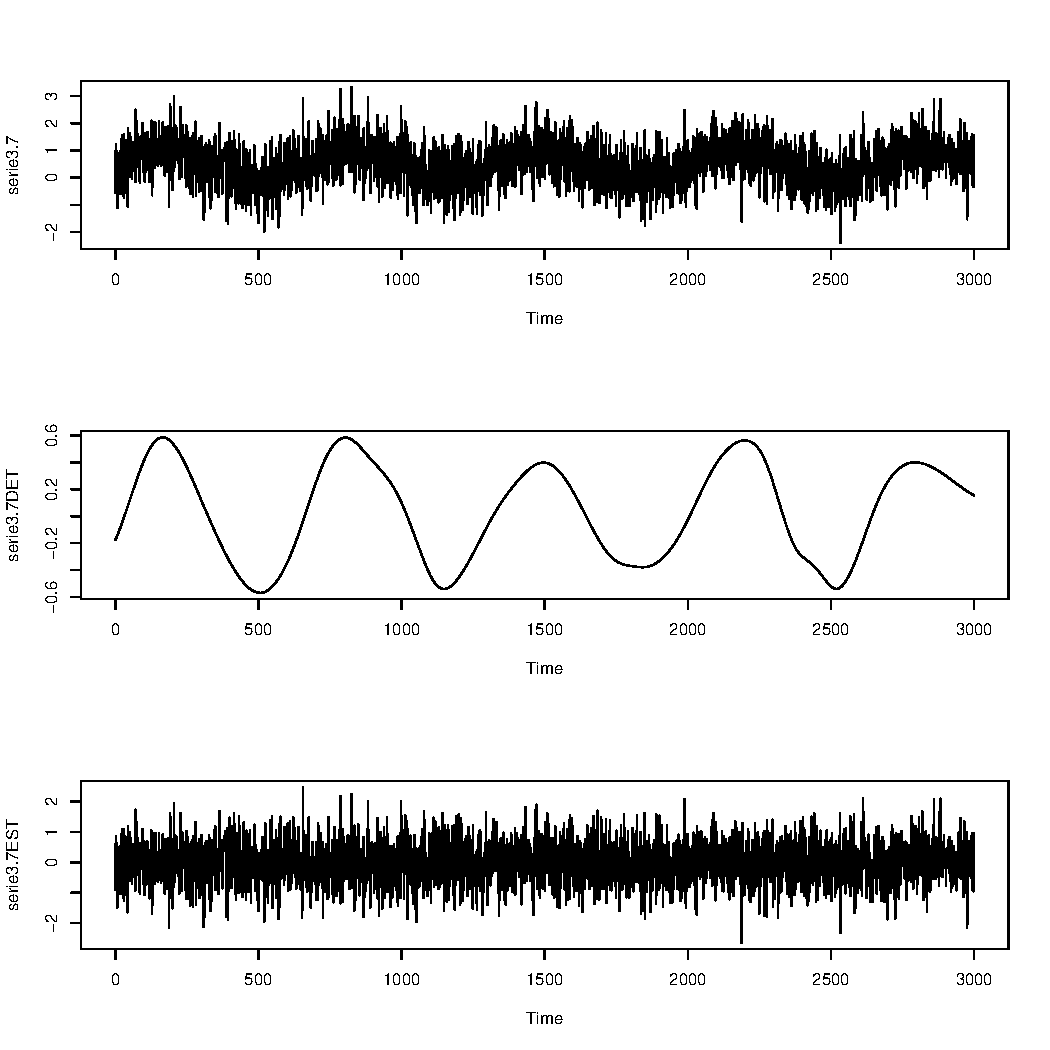
\includegraphics[scale=0.43]{serie3_7.pdf} \quad
  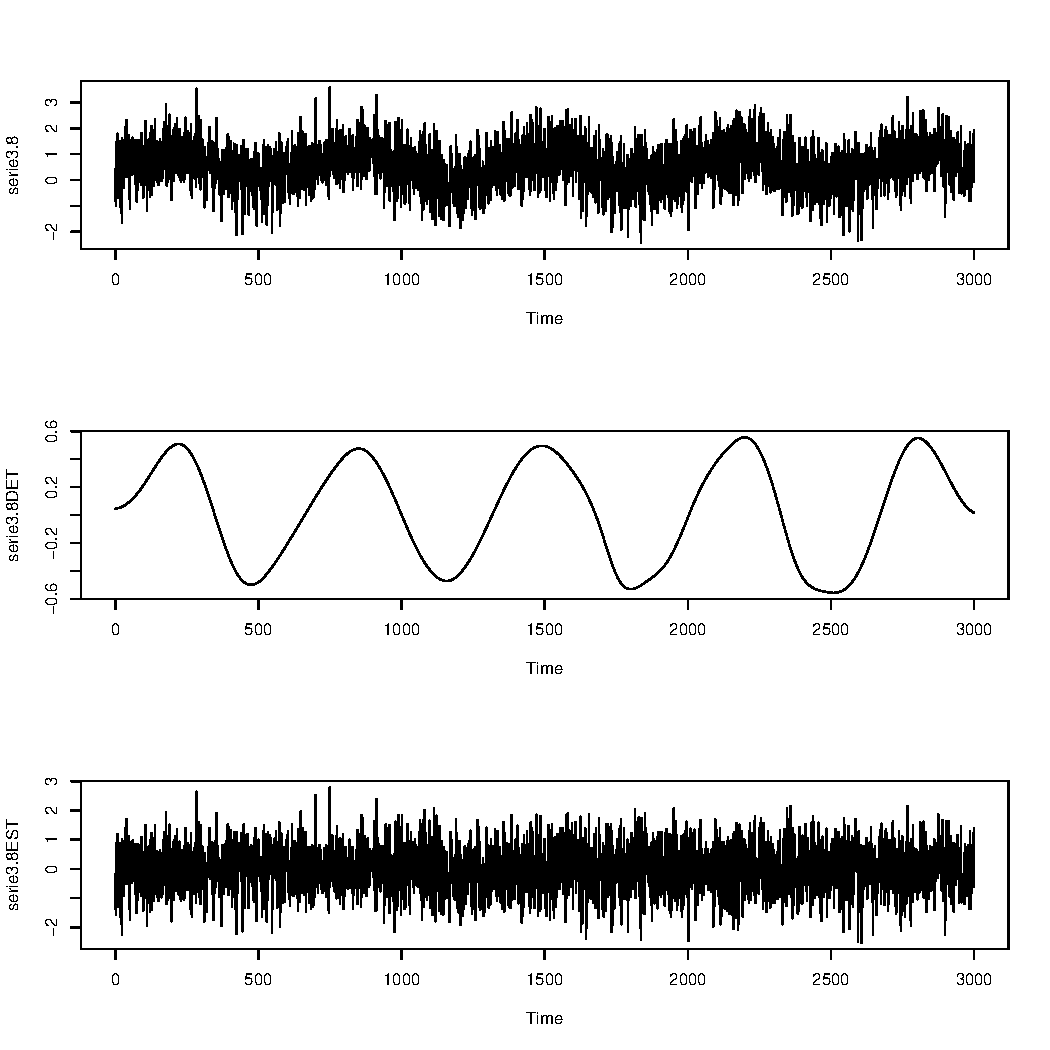
\includegraphics[scale=0.43]{serie3_8.pdf}
  \caption{Série 3.7 e Série 3.8}

\end{center}
\end{figure}

\graphicspath{{imagens/}}
\begin{figure}[H]
\begin{center}
  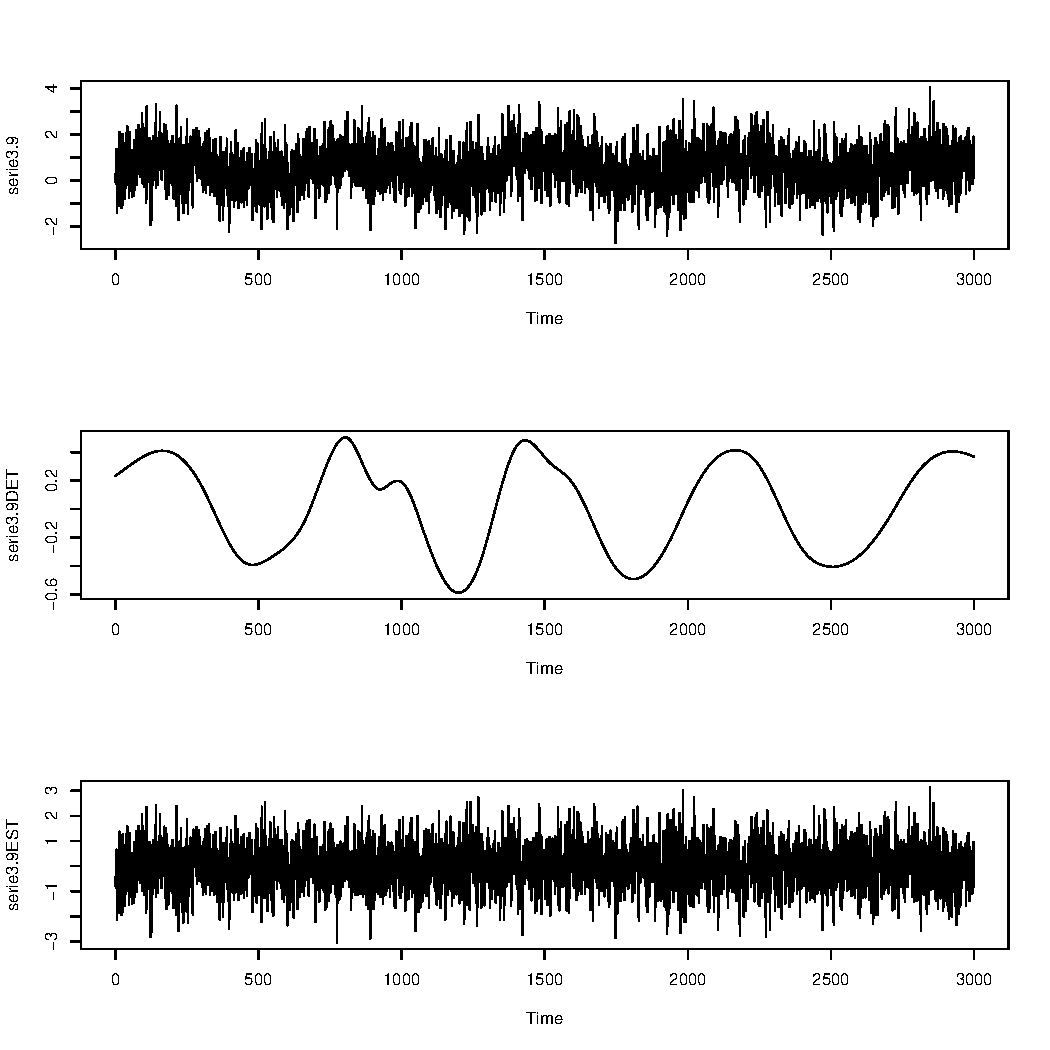
\includegraphics[scale=0.43]{serie3_9.pdf} \quad
  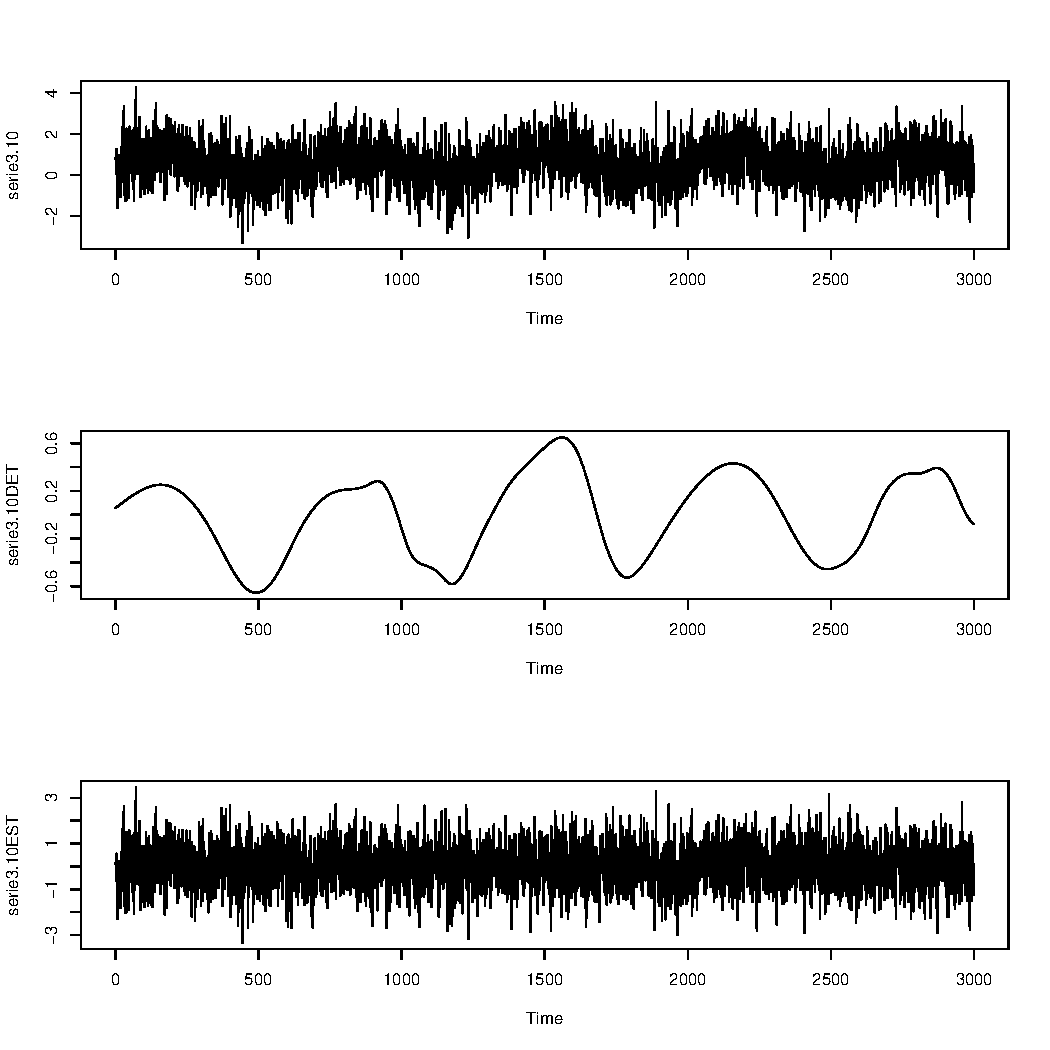
\includegraphics[scale=0.43]{serie3_10.pdf}
  \caption{Série 3.9 e Série 3.10}

\end{center}
\end{figure}

\section{Séries TIPO 4}
10 séries senoide com ruído ao longo da série e tendência.
\graphicspath{{imagens/}}
\begin{figure}[H]
\begin{center}
  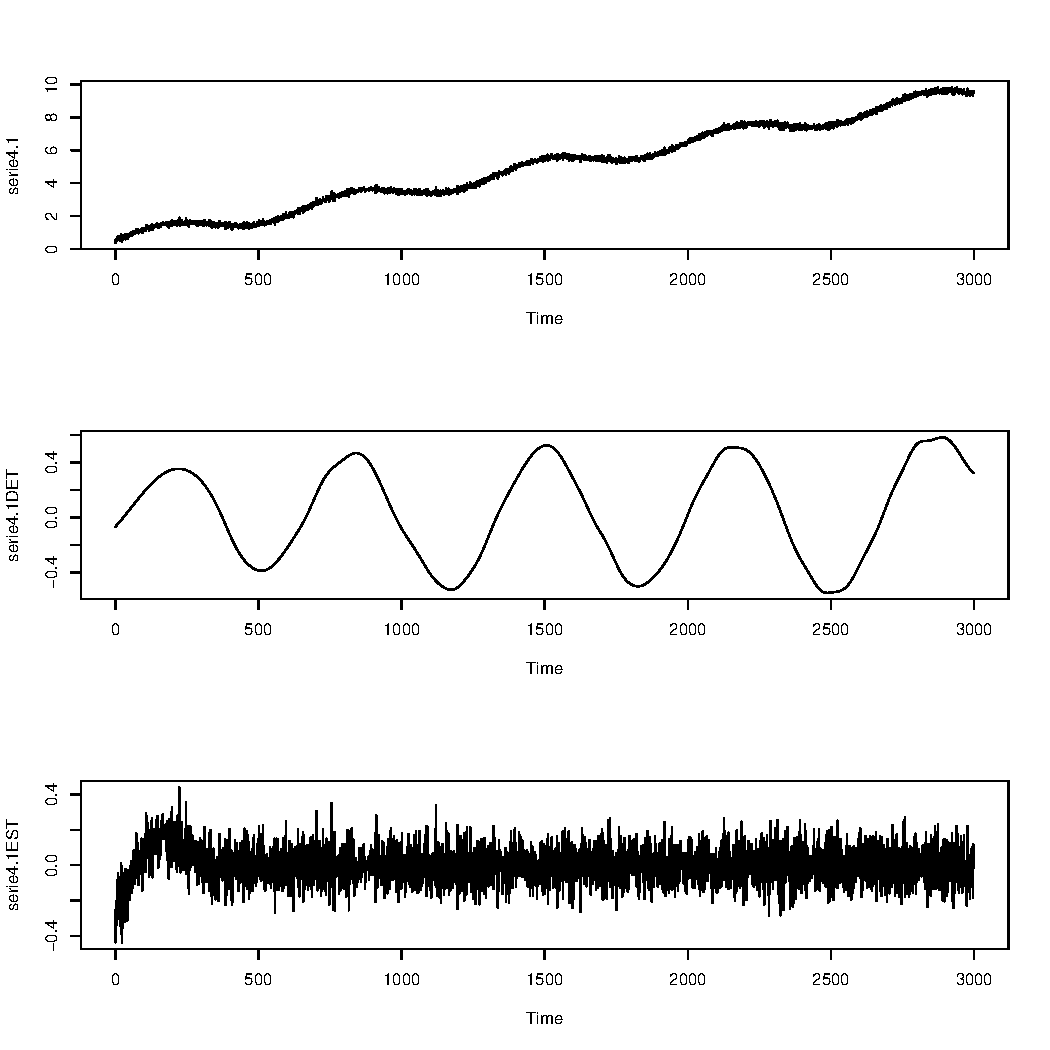
\includegraphics[scale=0.43]{serie4_1.pdf} \quad
  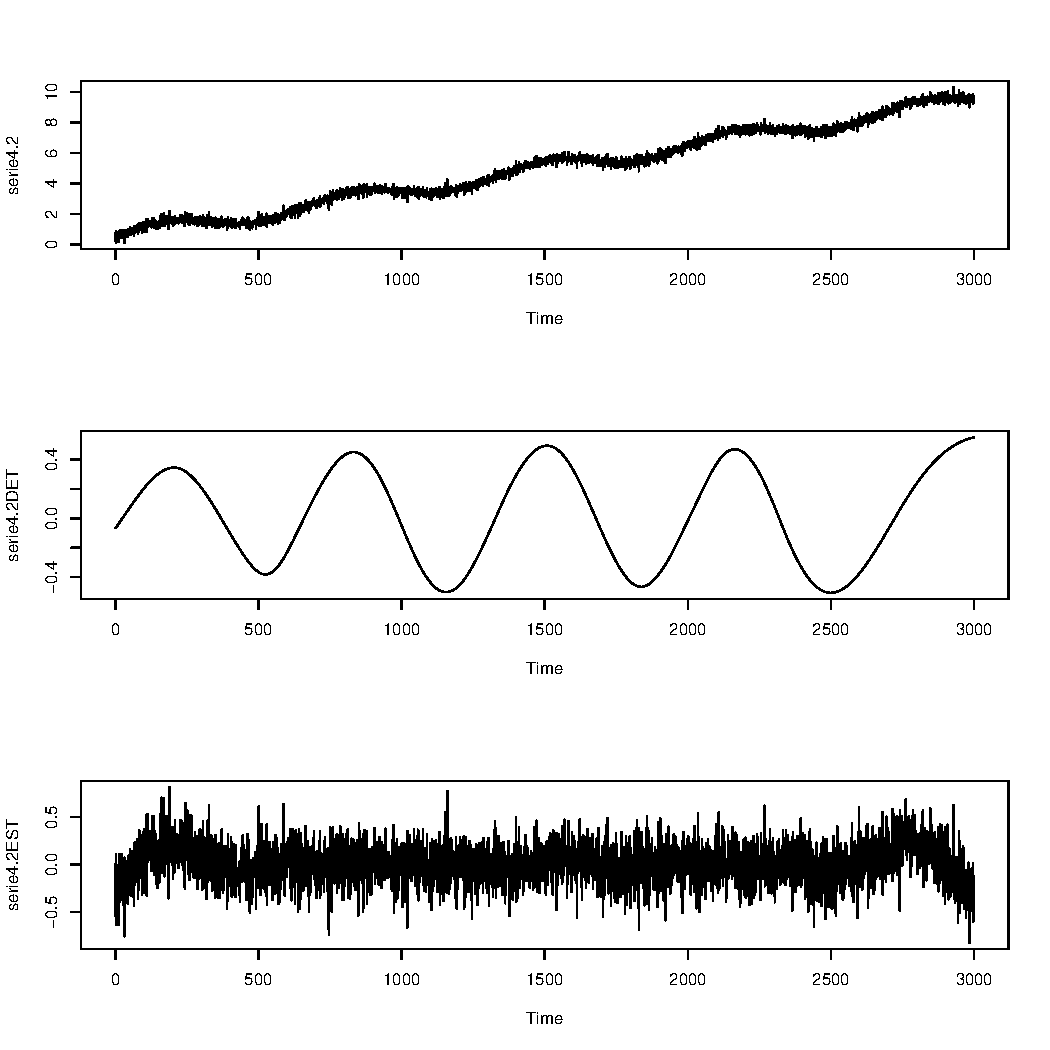
\includegraphics[scale=0.43]{serie4_2.pdf}
  \caption{Série 4.1 e Série 4.2}
\end{center}
\end{figure}

\graphicspath{{imagens/}}
\begin{figure}[H]
\begin{center}
  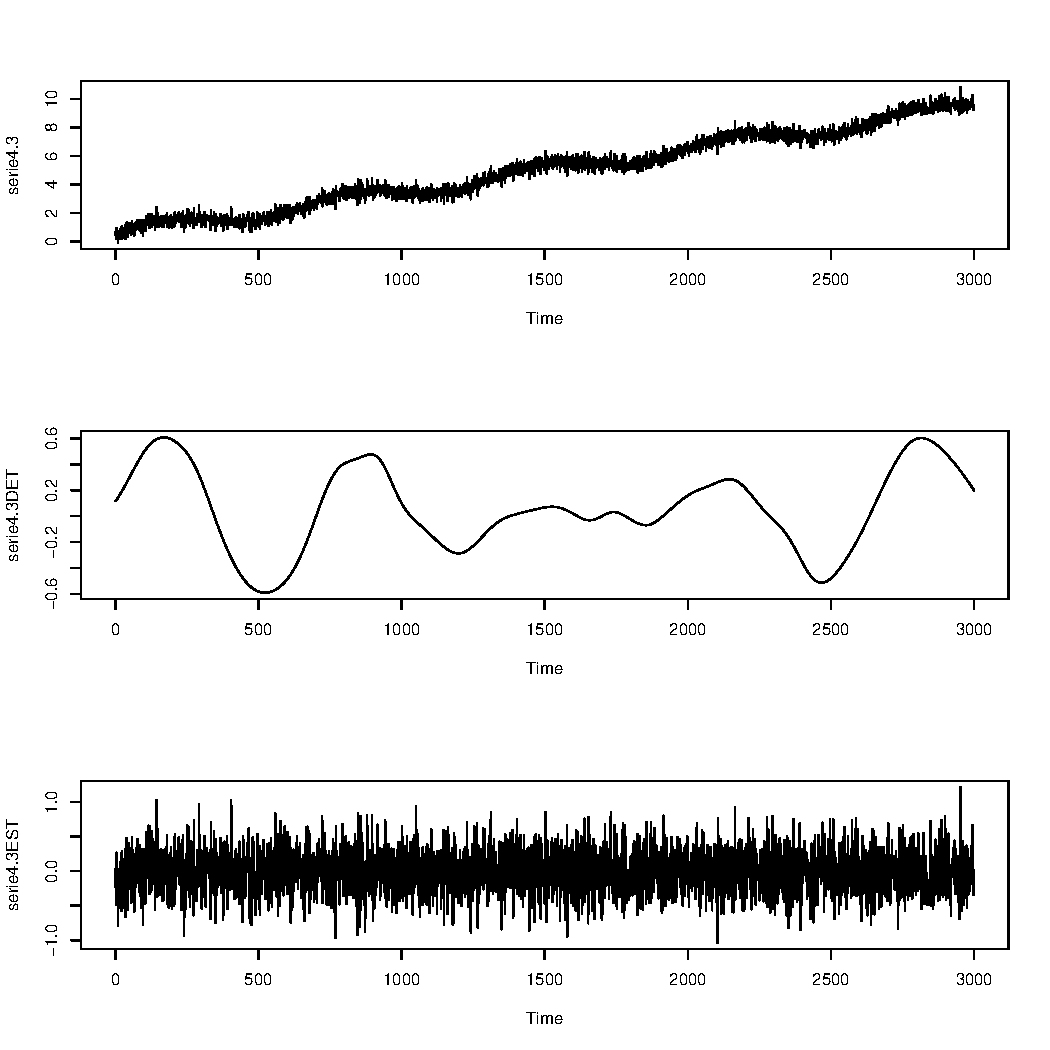
\includegraphics[scale=0.43]{serie4_3.pdf} \quad
 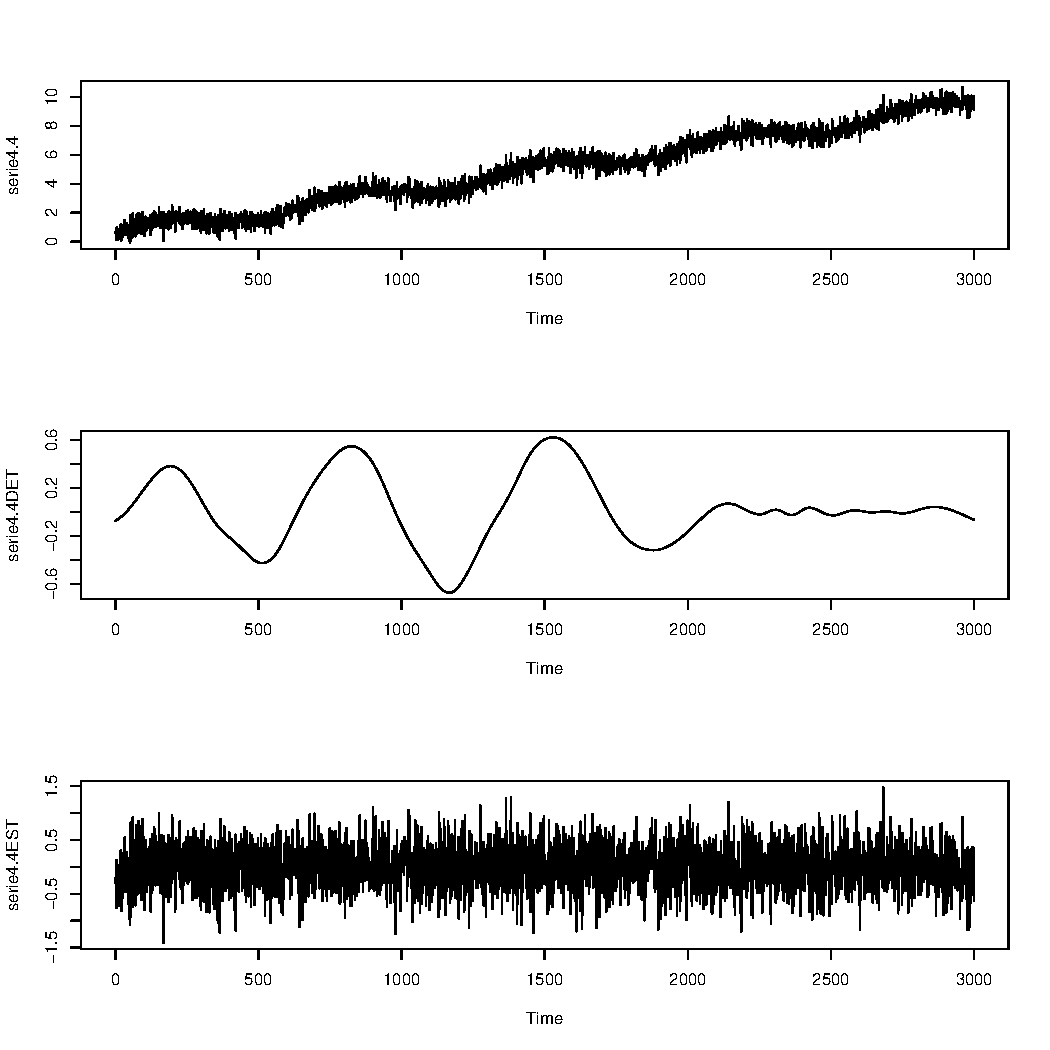
\includegraphics[scale=0.43]{serie4_4.pdf}
 \caption{Série 4.3 e Série 4.4}

\end{center}
\end{figure}

\graphicspath{{imagens/}}
\begin{figure}[H]
\begin{center}
  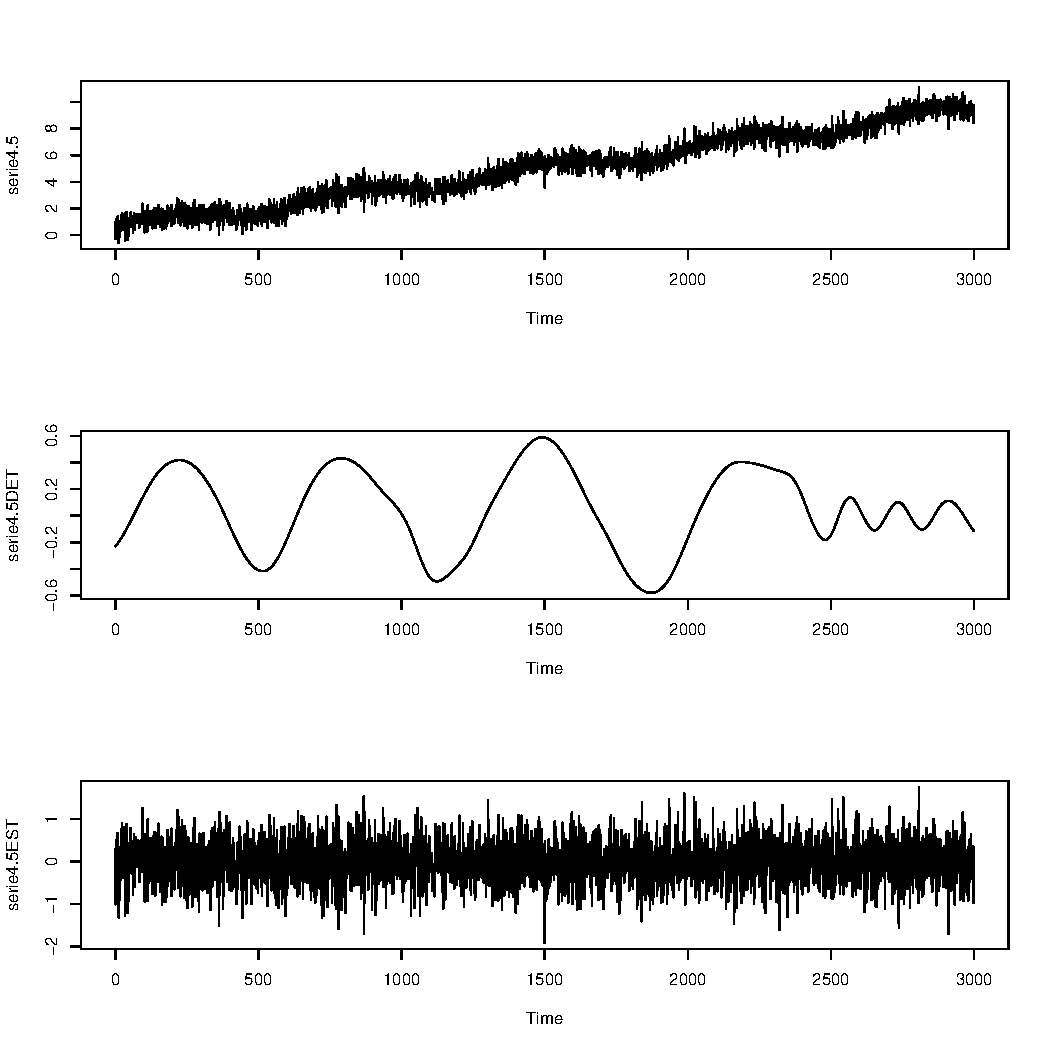
\includegraphics[scale=0.43]{serie4_5.pdf} \quad
  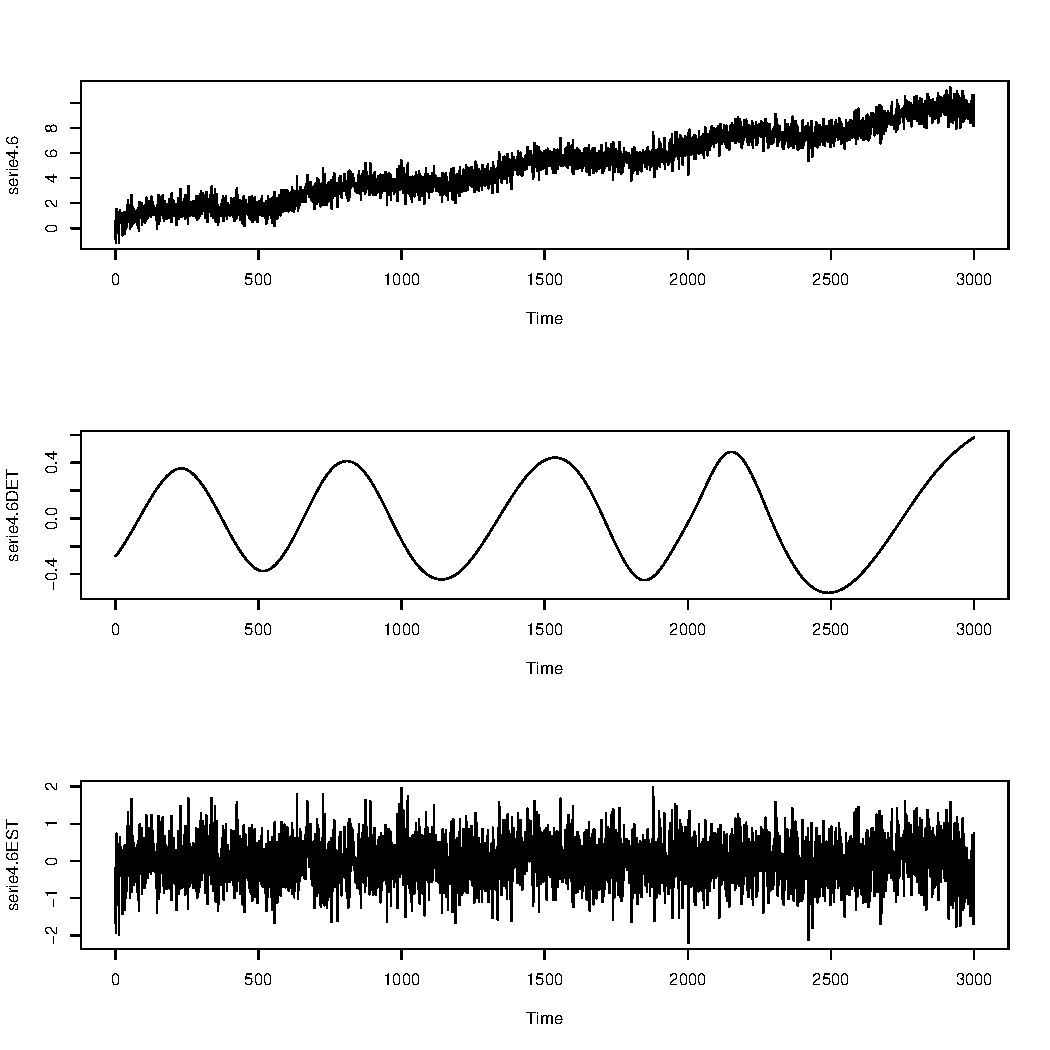
\includegraphics[scale=0.43]{serie4_6.pdf}
 \caption{Série 4.5 e Série 4.6}

\end{center}
\end{figure}

\graphicspath{{imagens/}}
\begin{figure}[H]
\begin{center}
  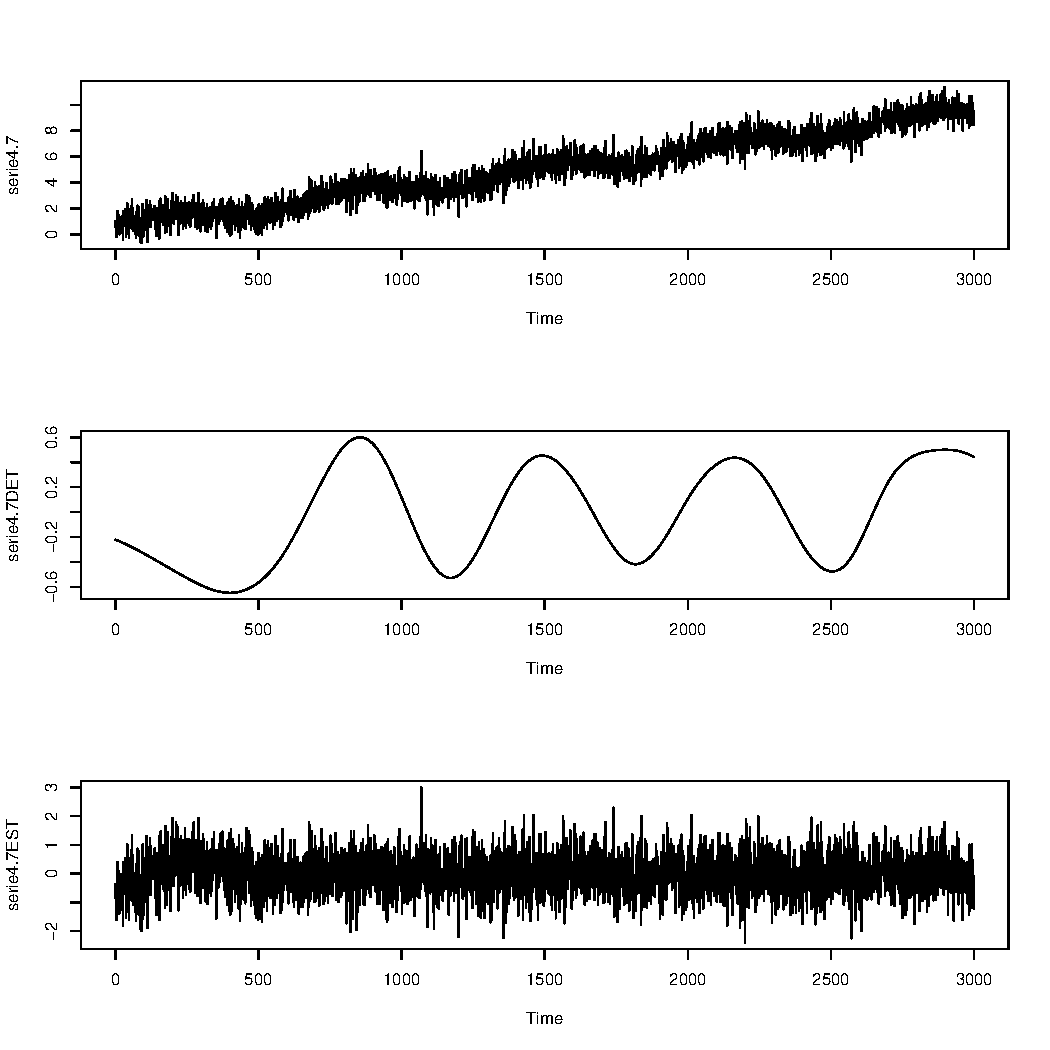
\includegraphics[scale=0.43]{serie4_7.pdf} \quad
  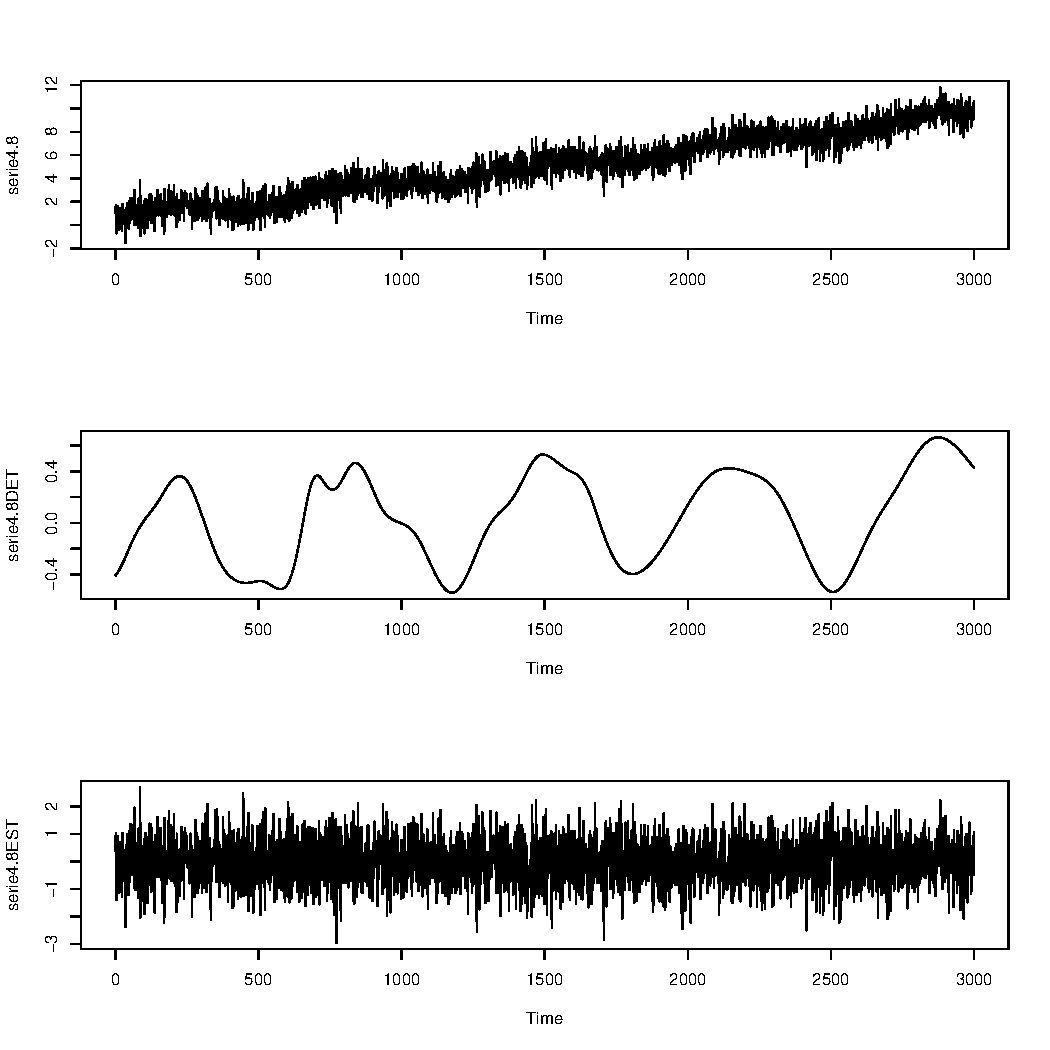
\includegraphics[scale=0.43]{serie4_8.pdf}
  \caption{Série 4.7 e Série 4.8}

\end{center}
\end{figure}

\graphicspath{{imagens/}}
\begin{figure}[H]
\begin{center}
  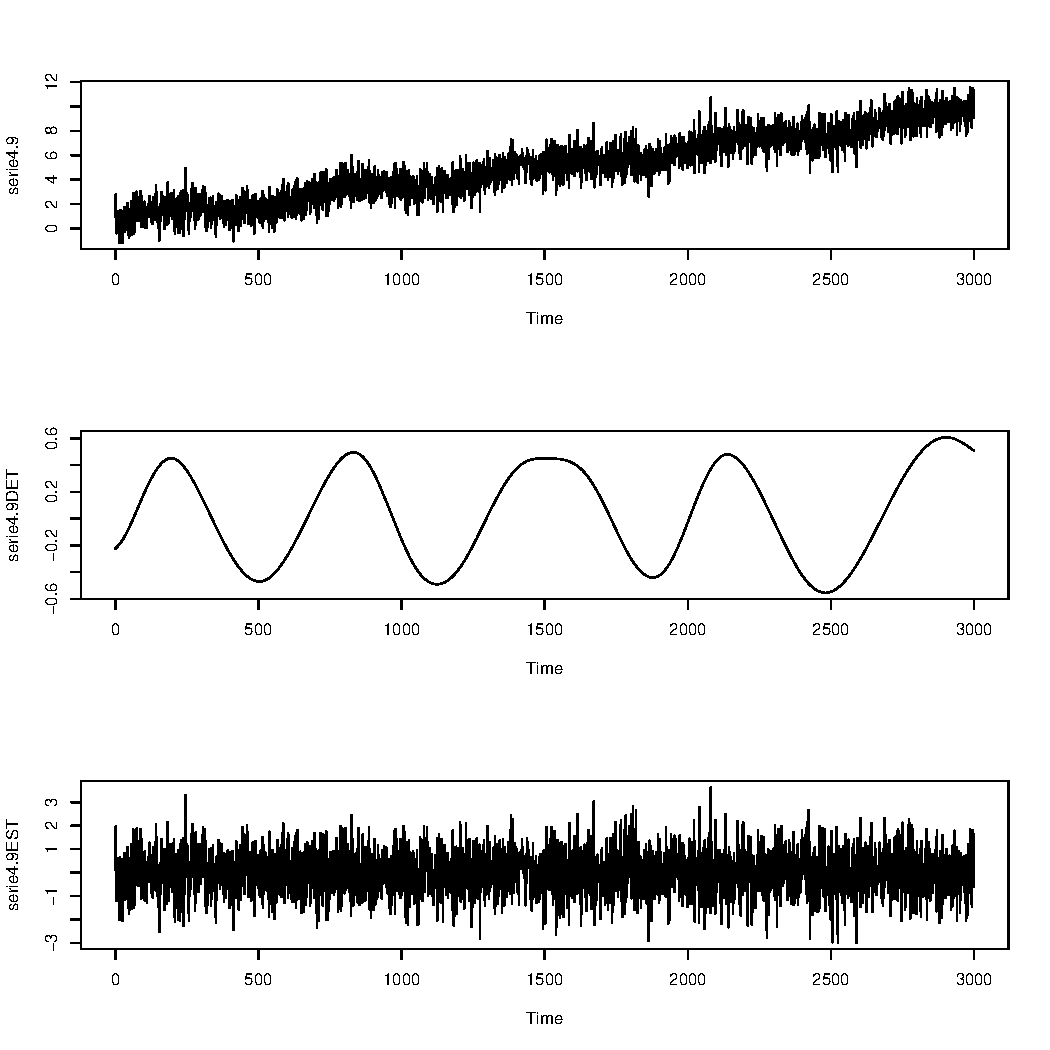
\includegraphics[scale=0.43]{serie4_9.pdf} \quad
  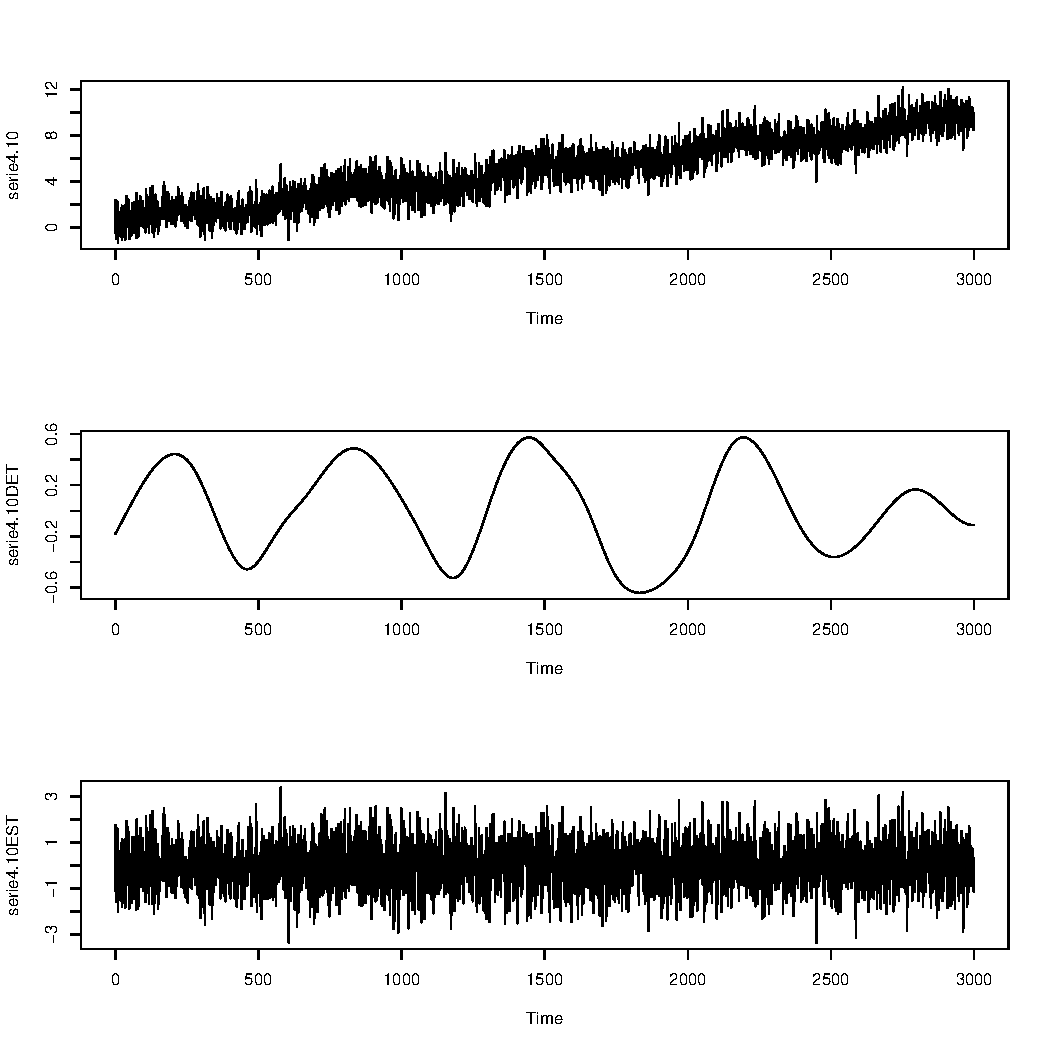
\includegraphics[scale=0.43]{serie4_10.pdf}
  \caption{Série 4.9 e Série 4.10}
\end{center}
\end{figure}
\section{Considerações Finais}
Foram apresentadas as séries temporais utilizadas neste trabalho experimental e suas respactivas decomposições.
% \include{apendice2}
% ...
% \include{apendiceM}

%% Fim do documento
\end{document}
%------------------------------------------------------------------------------------------%
